\documentclass[10pt]{article}

% Idioma y codificación
\usepackage[utf8]{inputenc}
\usepackage[spanish]{babel}

% Márgenes
\usepackage{geometry}
\geometry{top=2.5cm, bottom=2.5cm, left=2.5cm, right=2.5cm}

% Gráficos y Tablas
\usepackage{pdflscape}
\usepackage{graphicx}
\usepackage{amsmath}
\usepackage{pdfpages}
\usepackage{multicol}
\usepackage{float}
\usepackage[table]{xcolor} % UNA SOLA VEZ Y CON [table]
\usepackage{booktabs}
\usepackage{xltabular}
\usepackage{caption}
\usepackage{subcaption}
\usepackage{array}
\usepackage{multirow}

% Listings para código
\usepackage{listings}
\lstdefinestyle{terminal}{
	backgroundcolor=\color{gray!10},
	basicstyle=\ttfamily\small,
	keywordstyle=\color{blue},
	commentstyle=\color{gray},
	frame=single,
	columns=fullflexible,
	morecomment=[l]{//}
}
\lstset{
	inputencoding=utf8,
	extendedchars=true,
	literate={á}{{\'a}}1 {é}{{\'e}}1 {í}{{\'i}}1 {ó}{{\'o}}1 {ú}{{\'u}}1 {ñ}{{\~n}}1
	{Á}{{\'A}}1 {É}{{\'E}}1 {Í}{{\'I}}1 {Ó}{{\'O}}1 {Ú}{{\'U}}1 {Ñ}{{\~N}}1
	{¡}{{!`}}1 {¿}{{?`}}1
}
\lstset{
	language=Java,
	basicstyle=\ttfamily\footnotesize,
	keywordstyle=\color{blue}\bfseries,
	stringstyle=\color{red},
	commentstyle=\color{green!60!black},
	numbers=left, 
	numberstyle=\tiny\color{gray},
	stepnumber=1,
	frame=single, 
	breaklines=true,
	tabsize=4,        % <--- REDUCE EL TAMAÑO DEL TABULADOR AL ESTÁNDAR DE JAVA
	keepspaces=true,  % <--- MANTIENE LA INDENTACIÓN EXACTA DE TU ARCHIVO
	showtabs=false    % <--- EVITA QUE SE DIBUJEN SÍMBOLOS RAROS EN LOS TABS
}

% Hipervínculos
\usepackage[hidelinks]{hyperref}
\hypersetup{
	colorlinks=true,
	linkcolor=blue,
	filecolor=magenta,
	urlcolor=cyan,
}

% Encabezados y pies de página
\usepackage{fancyhdr}
\pagestyle{fancy}
\fancyhf{}
\fancyfoot[R]{\thepage}

% Formato de títulos
\usepackage{titlesec}
\titleformat{\subsection}{\normalfont\large\bfseries}{\thesubsection}{1em}{}
\titleformat{\subsubsection}{\normalfont\normalsize\bfseries}{\thesubsubsection}{1em}{}

% Datos de la portada
\title{\textit{CARD PARTNER}\\ Una web para amantes de los \textit{TCGS}}

\author{
	\textbf{\small ÁLVAREZ FULCONIS, MARCOS PALATINO}\\
	\textbf{\small LÓPEZ PRIMO, ÁLVARO}\\
	\textbf{\small OTERO GARCÍA, SERGIO}\\
	\textbf{\small SANTIESTEBAN MENDO, EDGAR}
}

\date{Curso 25-26}

\begin{document}
	
	\begin{titlepage}
		\centering
		% Asegúrate de que la ruta al PDF de la UVA sea correcta
		%
\includegraphics[scale=0.3]{./Recursos/UVA-3881270087.pdf}\\[0.5cm] 
		\rule{\linewidth}{0.2mm}\\[0.4cm]
		{\huge\bfseries CARD PARTNER\par}
		{\large Una web para amantes de los TCGS\par}
		\rule{\linewidth}{0.2mm}\\[1.5cm]
		{\Large\bfseries Servicios y Sistemas Web}\\[0.3cm]
		{\large\bfseries Laboratorio L2 \\ GRUPO 33}\\[1cm]
		{\Large \begin{tabular}{c} ÁLVAREZ FULCONIS, MARCOS \\ LÓPEZ PRIMO, ÁLVARO \\ OTERO GARCÍA, SERGIO \\ SANTIESTEBAN MENDO, EDGAR \end{tabular}}\\[1.5cm]
		{\Large Curso 25-26}
	\end{titlepage}
	
	\pagenumbering{gobble}
	\tableofcontents \newpage
	
	\pagenumbering{arabic} 
	\setcounter{page}{1}
	
	\section{Presentación del equipo}
	\textit{CardPartner} es la idea de página web que hemos desarrollado el Grupo 33 para la asignatura de Sistemas y Servicios Web.\\
	Este grupo está formado por Marcos Álvarez Fulconis, Álvaro López Primo, Sergio Otero García y Edgar Santiesteban Mendo.\\
	La motivación de nuestra web es simple, ofrecer una herramienta intuitiva, de fácil uso y accesible para todas aquellas personas interesadas en adentrarse en el mundo de los \textit{Trading Card Games} o TCGs, enfocándonos en el juego de cartas basado en el universo \textit{de One Piece}.\\
	
	\subsection{Organización del trabajo}
	Debido a la amplitud del proyecto, hemos estado empleando un repositorio \textit{Git} para poder paralelizar el trabajo. Hemos tenido dos fases de organización basándonos en la cantidad de tareas y el número de personas necesarias para cada una de ellas.\\
	
	\subsubsection{Primeras dos entregas}
	Durante las dos primeras entregas hemos optado por un enfoque mas grupal donde trabajábamos conjuntamente, ya que las primeras fases se basaban en maquetar el esqueleto de nuestra idea de página web.
	\begin{table}[H]
		\centering
		\begin{tabularx}{\textwidth}{llX} 
			\toprule
			\textbf{Nombre} & \textbf{Porcentaje} & \textbf{Responsabilidad principal} \\
			\midrule
			ÁLVAREZ FULCONIS, MARCOS PALATINO      	& 25\%                & Diseño de las vistas tcg, social,noticias,torneo y guías\\
			LOPEZ PRIMO, ÁLVARO      				& 25\%                & Diseño del index, login y todas sus opciones, creación del repositorio de github, redacción del documento\\
			OTERO GARCÍA, SERGIO     				& 25\%                & Diseño de decks y todos sus submenús, \textit{comunity decks, meta decks}, creación de mazos,vista de cartas\\
			SANTIESTEBAN MENDO, EDGAR    			& 25\%                & Modelo de dominio,flujos de navegación, requisitos y redacción del documento\\
			\bottomrule
		\end{tabularx}
		\caption{Distribución de responsabilidades y aporte de cada miembro en las dos primeras entregas de nuestra web \textit{Card Partner}}
	\end{table}
	De esta forma hemos conseguido plasmar los diferentes enfoques de cada uno de los integrantes del equipo, para así conseguir una web que cubra las diferentes necesidades que nos hemos ido encontrando a medida que investigábamos los \textit{TCGs}
	\subsubsection{Últimas dos entregas}
	En las fases finales del proyecto decidimos cambiar el enfoque empleado: optamos por dividirnos en equipos de dos personas en cada uno de ellos para poder acelerar el trabajo y permitir más independencia a la hora de realizar toma de decisiones.\\
	Los equipos se dividieron en base a como se ha realizado la implementación: \textit{frontend} y \textit{backend}.\\
	
	Los compañeros del \textit{frontend} se han encargado principalmente de la maquetación, el diseño visual, la navegación entre vistas y la implementación de las páginas JSP. Concretamente, han desarrollado vistas como la página principal, el catálogo de cartas, la visualización de las mismas, la sección de contenido social, el perfil de usuario, el login, el registro y todo lo relacionado con los mazos (la página de creación o construcción de los mismos, los mazos \textit{META} o los mazos generados por la comunidad).
	
	Por otra parte los compañeros del \textit{backend} se ha centrado en el diseño e implementación de la bbdd, la creación de los scripts SQL, la definición de las clases del modelo, la construcción de los DAOs, la implementación de los Servlets y la automatización de la creación de la base de datos en local. También se ha encargado de transformar los datos necesarios para poblar la aplicación y de preparar la conexión entre la capa de presentación y la capa de persistencia.
	\begin{table}[H]
		\centering
		\renewcommand{\arraystretch}{1.3}
		\begin{tabular}{|>{\centering\arraybackslash}p{4cm}|>{\centering\arraybackslash}p{2cm}|p{8cm}|}
			\hline
			\textbf{Nombre} & \textbf{Porcentaje} & \textbf{Responsabilidad principal} \\
			\hline
			\multicolumn{3}{|c|}{\textbf{Equipo Frontend}} \\
			\hline
			Marcos Álvarez Fulconis & 25\% & Desarrollo de vistas relacionadas con cartas y apartado social, apoyo en la navegabilidad general de la aplicación, revisión visual de las páginas y maquetación del documento. \\
			\hline
			Sergio Otero García & 25\% & Desarrollo de vistas relacionadas con mazos, login, registro, página principal y constructor de mazos. Apoyo en la redacción del documento y en la integración visual de las distintas secciones. \\
			\hline
			\multicolumn{3}{|c|}{\textbf{Equipo Backend y Gestión de Datos}} \\
			\hline
			Álvaro López Primo & 25\% & Creación del esquema de la base de datos, colaboración en el modelo entidad-relación, población de la base de datos, transformación de datos externos y automatización de scripts para MariaDB en local. Apoyo en la redacción técnica del documento. \\
			\hline
			Edgar Santiesteban Mendo & 25\% & Colaboración en el modelo entidad-relación, creación de esquemas de base de datos, desarrollo de clases del modelo, DAOs y DTOs, y apoyo en la redacción técnica del documento. \\
			\hline
		\end{tabular}
		\caption{En esta tabla se refleja el enfoque de las últimas dos entregas y la aportación de cada uno de los integrantes del grupo 33}
	\end{table}
	\subsection{Justificación este cambio de enfoque}
	El cambio de nuestra manera de trabajar se debe a la amplitud del proyecto. Nuestra web requiere de una interfaz visual amplia, con múltiples vistas para cartas, mazos, perfil, noticias, guías y torneos, pero a su vez necesita una base de datos consistente y una lógica de servidor capaz de gestionar usuarios, cartas, mazos, comentarios, valoraciones y contenido editable.\\
	
	Separar las responsabilidades nos ha permitido avanzar de forma más ordenada y nos ha ayudado a focalizar el trabajo individual, ya que cada uno de los equipos tenía una visión clara de la lista de tareas que debían realizar.\\
	
	Esta metodología también nos ha facilitado la implemetación de mejoras y corrección de errores vistos en el \textit{feedback} de entregas anteriores. Por ejemplo, hemos incorporado una vista de perfil del usuario más completa, hemos desarrollado mejor la distinción entre mazos de comunidad y mazos meta, y hemos consolidado la existencia de usuarios con distintos roles dentro del sistema. Además, la creación de scripts de automatización para la base de datos nos ha permitido que todos los miembros puedan trabajar con una estructura local equivalente, evitando problemas derivados de no disponer de un servidor remoto común.
	
	
	%-------------------------------- COMPROBAR SI SOBRA ESTA PARTE POR REPETICION ------------------------%
	
	% \subsection{Evolución del trabajo respecto a entregas anteriores}
	%     El proyecto ha evolucionado de manera progresiva. En la primera entrega trabajamos principalmente sobre la idea inicial, el análisis del problema y los primeros bocetos. En la segunda entrega formalizamos el sistema mediante requisitos, modelo de dominio y mapa de navegación. En la tercera entrega avanzamos hacia una implementación funcional, incorporando JSP, CSS, Servlets, DAOs, clases de dominio y scripts SQL.\\
	
	%     Esta evolución nos ha permitido transformar \textit{Card Partner} de una propuesta conceptual a una aplicación web con una estructura técnica más completa. El resultado final mantiene la idea inicial de centralizar herramientas útiles para jugadores de TCG, pero incorpora una arquitectura más definida, una base de datos relacional, una separación clara entre vistas y lógica de servidor, y una organización más precisa de los distintos módulos de la plataforma.
	\newpage
	\section{Contexto y problema abordado}        
	El mundo de los TCG, o \textit{Trading Card Games}, ha crecido notablemente en los últimos años y cada vez reúne a más jugadores con perfiles muy distintos. Algunos usuarios se acercan por primera vez al juego y necesitan aprender sus reglas básicas, mientras que otros son eruditos de las mecánicas y buscan herramientas para consultar mazos competitivos, estudiar cartas, revisar precios o compartir sus propios mazos con la comunidad.\\
	
	Gran parte del grupo 33 está comenzando a jugar a este tipo de juegos de cartas y nos hemos encontrado muchos problemas a la hora de introducirnos en este mundillo. El principal problema encontrado es la cantidad abrumadora de información que hay sobre estos juegos, añadiendo que pocos sitios web centralizan la información de una manera clara y accesible para personas novatas en estos \textit{hobbies}. Ya no sólo basta con buscar información sobre el META (\textit{Most Effective Tactics Available}), sino también el precio de las cartas que constituyen los mazos, donde se pueden adquirir las mismas o el circuito competitivo del mismo.\\
	
	Por este motivo, hemos decidido plantear \textit{Card Partner} como una aplicación web centralizada \textit{All In One}, tanto para jugadores recién iniciados como veteranos aficionados a los TCG, reuniendo en un mismo sitio funcionalidades como  la consulta de cartas, visualización de sus precios, creación y gestión de mazos, consulta de mazos META, noticias, guías, torneos y funcionalidades sociales como comentarios, valoraciones y mazos guardados.\\
	
	Emplearemos como eje central el TCG basado en la serie japonesa \textit{One Piece} por dos motivos: el primero es para acotar el problema, ya que existen cientos de juegos diferentes, cada uno con sus cartas y mecánicas, y si no tomamos uno como referencia para nuestra web tendríamos un problema inabarcable para 4 personas; el segundo es que es el TCG con el que más familiarizados estamos, gracias a que muchos de los miembros de este grupo somos, o jugadores experimentados en el juego o fanáticos del universo de la obra.
	\newpage
	\subsection{Análisis de soluciones existentes}   \label{ASE}
	Como ya hemos planteado en la sección anterior, ya existen aplicaciones web con un enfoque similar a lo que estamos planteando para esta entrega, por lo que hemos realizado un pequeño análisis de las mismas para ver sus fortalezas y debilidades.
	\begin{table}[H]
		\centering
		\renewcommand{\arraystretch}{1.3}
		\begin{tabular}{|p{3.2cm}|p{5.2cm}|p{5.2cm}|}
			\hline
			\textbf{Plataforma} & \textbf{Fortalezas} & \textbf{Limitaciones detectadas} \\
			\hline
			\href{https://www.cardmarket.com/es/OnePiece}{\textit{Card Market}} & Es una de las plataformas más completas para consultar precios y realizar compraventa de cartas de distintos TCG. & Está orientada principalmente al mercado de cartas, por lo que no ofrece una experiencia centrada en la creación de mazos, el aprendizaje del juego o la interacción entre usuarios. \\
			\hline
			\href{https://deckbuilder.egmanevents.com/optcg/cards}{\textit{EggmanEvents}} & Permite consultar mazos utilizados en torneos y resulta útil para jugadores interesados en el entorno competitivo. & Su enfoque está muy ligado a resultados competitivos. Además, puede resultar menos intuitiva para usuarios novatos y no está orientada a que el usuario cree, gestione y comparta sus propios mazos. \\
			\hline
			\href{https://en.onepiece-cardgame.com/beginners/}{\textit{One Piece Card Game}} & Es la fuente más fiable para consultar productos oficiales, reglas básicas y materiales introductorios del juego. & No funciona como comunidad de usuarios ni ofrece herramientas completas para construir mazos, valorar listas, guardar contenido personalizado o consultar precios de mercado. \\
			\hline
			
			\href{https://onepiece.limitlesstcg.com}{\textit{One Piece Limitless}} & Reúne información competitiva, estadísticas de torneos, cartas y herramientas relacionadas con el juego. & Aunque ofrece información útil para jugadores avanzados, no centraliza en una misma experiencia el aprendizaje para principiantes, la gestión personal de mazos, los precios y la interacción social. \\
			\hline
		\end{tabular}
		\caption{Comparación de plataformas existentes relacionadas con \textit{One Piece} TCG}
	\end{table}     
	\newpage
	\section{\textit{CardPartner} como idea general}        
	Esta revisión nos ha permitido tener muy claro el enfoque que le queremos dar a nuestra aplicación web
	con esa visión \textit{All in One} que hemos comentado en el primer punto de este informe.\\
	
	Nuestra aplicación permitirá a los usuarios realizar las siguientes acciones principales:
	\begin{itemize}
		\item \textbf{Consultar el catálogo de cartas:} navegar por todas las cartas existentes del juego.
		\item \textbf{Acceder al detalle de cada carta:} revisar información específica de una carta concreta, como el tipo, color, coste, poder y precio de mercado.
		\item \textbf{Crear mazos:} emplear el catálogo como base para la construcción de nuevas barajas jugables.
		\item \textbf{Explorar el módulo de mazos:} sección específica que clasifica las construcciones en dos categorías:
		\begin{itemize}
			\item Los \textbf{mazos de la comunidad}, que representan listas creadas y compartidas por usuarios.
			\item Los \textbf{mazos meta}, que permiten destacar construcciones competitivas o recomendadas por sus resultados.
		\end{itemize}
		\item \textbf{Interactuar entre miembros de la comunidad:} posibilidad de que los usuarios puedan comentar, valorar y guardar los mazos de la plataforma.
		\item \textbf{Acceder a contenido editorial:} secciones dedicadas a noticias, guías y torneos, pensadas para mantener al usuario informado y facilitar la entrada de jugadores principiantes al TCG.
		\item \textbf{Gestionar la cuenta de usuario:} opciones para registrar cuentas, iniciar sesión, gestionar el perfil y acceder a funcionalidades personalizadas. Esto permite diferenciar la experiencia de un visitante no registrado de la de uno que sí lo está, puesto que estos últimos tienen la capacidad de crear, guardar y gestionar su propio contenido.
	\end{itemize}
	
	Con esto conseguimos que la aplicación sea útil tanto para jugadores con un perfil más competitivo o veteranos en este juego como para aquellos que no cuenten con tanta experiencia.\\
	
	Llegados a este punto, nos podemos preguntar ¿qué aporta \textit{Card Partner} al mercado de las aplicaciones web de TCGs? \\
	
	La respuesta a esta cuestión es la siguiente: la interacción entre miembros de la comunidad en una web especializada, ya que es una \textit{feature} muy poco desarrollada en este mundillo. Como equipo de desarrollo consideramos que el hecho de tener una aplicación útil es tan importante como el de tener una comunidad sana, que dispongan de una plataforma para ayudarse mutuamente, compartir conocimiento y valoraciones sobre mazos o líderes. El éxito de un TCGs no se basa en la calidad de los artes (las ilustraciones de las cartas) o la jugabilidad, si no en tener una comunidad activa la cual cuente con espacios para poder disfrutar y compartir su pasatiempo con todo aquel que comparta sus mismos gustos.\\
	
	
	%• El grupo de usuarios a que se destine el sitio web debe ser sensato y no trivial.
	%• Se describirá el grupo de usuarios con suficiente detalle como para poder diferenciarlo de otros.
	%• Se describirán las necesidades y expectativas reconocidas en el grupo de usuarios objetivo.
	% USUARIOS (6,5/10)\\
	% Se definen dos tipos de usuario a nivel de 'usuarios finales', con los perfiles claramente definidos. No se cita ningún tipo de usuario con capacidad de administración de la aplicación a nivel de 'backend'/mantenimiento. ¿Existe? Se debe concretar, ya que se está diseñando una aplicación que, posiblemente, requerirá mantenimiento y/o actualizaciones, gestión de los contenidos,... ¿Quién lo lleva a cabo?\\
\newpage
	\section{Usuarios objetivo}       
	Teniendo en mente la idea y las funcionalidades que deberá tener nuestra aplicación web, vamos a analizar los usuarios objetivos para la misma.
	A continuación listaremos y añadiremos una pequeña descripción de los usuarios prototípicos de nuestra aplicación, aunque profundizaremos en cada uno de ellos en sus respectivos apartados más adelante. Consideramos que es importante tener una visión global de los mismos así como su clasificación.
	\begin{table}[H]
		\centering
		\renewcommand{\arraystretch}{1.5} % Da un poco de aire entre las filas
		\begin{tabularx}{\textwidth}{|>{\raggedright\arraybackslash}p{3cm}|>{\raggedright\arraybackslash}p{4cm}|>{\raggedright\arraybackslash}X|}
			\hline
			\textbf{Clasificación} & \textbf{Perfil de Usuario} & \textbf{Descripción, Necesidades y Expectativas} \\
			\hline
			\multirow{2}{=}{\textbf{Según conocimiento del juego}} 
			& \textbf{Principiante / Casual} & Jugador que recién comienza en el TCG. \textbf{Necesidades:} interfaz intuitiva, acceso fácil a guías, tutoriales y mazos recomendados para aprender a jugar. \textbf{Expectativas:} encontrar un entorno amigable que facilite, tanto por la información disponible como por la comunidad de la web,su curva de aprendizaje sin abrumarle con datos complejos. \\
			\cline{2-3}
			& \textbf{Experimentado / Competitivo} & Jugador habitual que busca optimizar sus estrategias. \textbf{Necesidades:} filtros avanzados en el catálogo de cartas, acceso detallado a \textit{mazos meta} y herramientas precisas para la construcción de sus propias barajas. \textbf{Expectativas:} información actualizada sobre el estado competitivo del juego. \\
			\hline
			\multirow{3}{=}{\textbf{Según nivel de acceso}} 
			& \textbf{Visitante no registrado} & Usuario que accede a la plataforma de forma anónima. \textbf{Necesidades:} consultar el catálogo de cartas, leer noticias y ver mazos públicos de la comunidad o meta. \textbf{Expectativas:} navegación rápida y sin fricciones como primera toma de contacto con la aplicación. \\
			\cline{2-3}
			& \textbf{Jugador registrado} & Usuario con cuenta activa en la plataforma. \textbf{Necesidades:} todas las del visitante no registrado, más la capacidad de crear, guardar y editar mazos, además de interactuar socialmente (comentar, valorar mazos de otros). \textbf{Expectativas:} disponer de un espacio personal seguro y persistente donde gestionar su progresión y creaciones, así como poder participar de la comunidad de los \textit{TCGs} \\
			\cline{2-3}
			& \textbf{Administrador o Mantenimiento} & \textit{Perfil de backend}. Usuario encargado de la gestión integral de la plataforma. \textbf{Necesidades:} acceso a un panel de control (backoffice) para actualizar el catálogo de cartas (nuevas expansiones), redactar y publicar noticias/guías, y moderar el contenido de la comunidad. \textbf{Expectativas:} herramientas eficientes y seguras para garantizar que la plataforma esté siempre actualizada, estable y libre de contenido inapropiado. \\
			\hline
		\end{tabularx}
		\caption{Resumen y definición de los perfiles de usuario de \textit{Card Partner}.}
		\label{tab:perfiles_usuario}
	\end{table}
	
	\subsection{Usuarios según su conocimiento del juego}
	Esta primera definición nos permite diferenciar dos grandes grupos de usuarios, los \textit{casuals} (termino empleado para definir a aquellas personas que conocen del juego pero no están interesados en el entorno competitivo) y los usarios competitivos o \textit{tryhards}. \\ 
	\begin{itemize}
		\item Para los  usuarios novatos hemos planteado secciones de guías, recomendaciones y mazos orientados a principiantes, de forma que puedan entender las reglas básicas, las mecánicas principales y las primeras decisiones necesarias para empezar a jugar.
		\item Para los  jugadores experimentados \textbf{Card Partner} ofrece funcionalidades como el apartado de noticias, el catálogo de cartas, el constructor de mazos, los mazos de la comunidad, los mazos meta, los comentarios y las valoraciones. Con ello, hemos buscado facilitar tanto el seguimiento del entorno competitivo como la interacción entre jugadores.
	\end{itemize}
	
	\subsection{Usuarios según su nivel de acceso}
	Además del tipo de usuario, tenemos que tener en cuenta las funcionalidades que va a poder realizar sobre nuestro sistema en función del nivel de acceso con el que cuente. Concretamente, tenemos 3 niveles diferentes, los visitantes (aquellos usuarios que no tienen cuenta), los que se encuentran registrados y por último los administradores de \textit{Card Partner}.
	\begin{itemize}
		\item \textbf{Usuario \underline{NO} registrado}: en esta clasificación encontramos a todos aquellos usuarios que no tienen una cuenta instanciada en nuestra aplicación web. Por este motivo, tienen acceso a funcionalidades limitadas, entre las que nos encontramos: consultar el catálogo de cartas, las noticias, guías, información sobre torneos, los mazos meta y los mazos publicados por la comunidad sin la posibilidad de interactuar con ellos (comentarlos, valorarlos, etc.). Su objetivo principal es explorar el contenido disponible antes de decidir si quiere registrarse.\\
		Pese a no tener acceso a todas las funcionalidades de nuestra web, su experiencia ha de ser satisfactoria puesto que el motivo para visitarnos es obtener información, ya sea de manera puntual o continuada.
		\item \textbf{Usuario \underline{SI} registrado}: aquel que ha creado una cuenta e iniciado sesión en la aplicación. Este tipo de usuarios a mayores de las opciones disponibles para los no registrados cuenta con funcionalidades personalizadas, como la gestión del perfil, la creación de mazos, el guardado de mazos, la publicación de listas y la posibilidad de realizar comentarios así como la valoración de mazos creados por otros usuarios.\\
		Este tipo de usuario constituye el núcleo de la comunidad de Card Partner, puesto que toda la aplicación gira alrededor a estos (gracias al especial hincapié que hemos hecho en el apartado de mazos y al entorno social).
		\item \textbf{Administrador o usuario de mantenimiento}: representa al usuario con los permisos de gestión y mantenimiento dentro de la aplicación, gestionar el contenido de la web, publicar noticias, actualizar el catálogo de cartas o de mazos metas (tareas que, en ningún momento, puedan realizar los dos tipos de usuarios mencionados anterioremente).\\
		Entre sus funciones se encuentran la gestión de contenidos editoriales como noticias, guías y torneos; la revisión de información relevante para la plataforma, la actualización de mazos oficiales o meta y el mantenimiento general de los datos del sistema. De esta forma, el administrador actúa como responsable de que la información publicada sea coherente, esté actualizada y mantenga la calidad esperada.
	\end{itemize}
	
%	\subsubsection{Usuario \underline{no} registrado}
%	En esta clasificación encontramos a todos aquellos que no tienen una cuenta en nuestra apliación web. Por este motivo, tiene funciones limitados las cuales son: consultar el catálogo de cartas, las noticias, guías, información sobre torneos, los mazos meta y los mazos publicados por la comunidad. Su objetivo principal es explorar el contenido disponible antes de decidir si quiere registrarse.\\
%	Pese a no tener acceso a todas las funcionalidades de nuestra web, su experiencia ha de ser satisfactoria, ya que su motivo para visitarnos es obtener información ya sea de manera puntual o continuada.
%	
%	\subsubsection{Usuario registrado}
%	Aquel que ha creado una cuenta e iniciado sesión en la aplicación. Este perfil dispone de funcionalidades personalizadas, como la gestión del perfil, la creación de mazos, el guardado de mazos, la publicación de listas, la posibilidad de realizar comentarios así como la valoración de mazos creados por otros usuarios.\\
%	
%	Este tipo de usuario constituye el núcleo de la comunidad de Card Partner, puesto que toda la aplicación gira entorno a estos, debido al especial incapie que hemos hecho en el apartado de mazos y al entorno social.
%	
%	\subsubsection{Administrador o usuario de mantenimiento}
%	Representa al usuario con permisos de gestión y mantenimiento dentro de la aplicación, acciones como gestionar el contenido de la web, publicar noticias, actualizar el catálogo de cartas o de mazos metas no deben depende en ningún momento de los dos tipos de usuarios mencionados anterioremente.\\
%	Entre sus funciones se encuentran la gestión de contenidos editoriales, como noticias, guías y torneos; la revisión de información relevante para la plataforma; la actualización de mazos oficiales o meta; y el mantenimiento general de los datos del sistema. De esta forma, el administrador actúa como responsable de que la información publicada sea coherente, esté actualizada y mantenga la calidad esperada.\\
	
	\newpage
	\section{Especificación de requisitos}
	En este apartado entraremos más en detalle sobre las características que vamos a desarrollar en nuestra aplicación web para poder satisfacer las demandas de los diferentes usuarios.\\
	% La especificación de requisitos está organizada y numerada en bloques temáticos, y contiene RNF específicos y mensurables.\\
	
	% El modelo de dominio es el que está mejor resuelto: la herencia adecuada de Usuario en Jugador y Administrador, una clase asociativa Contiene con un atributo cantidad, enumeraciones particulares del dominio (tipos, colores,...), y una descripción textual que complementa de manera perfecta el diagrama.\\
	
	% El mapa del sitio, que documenta cuatro niveles de profundidad con flujos de navegación detallados, excede lo común en esta entrega. La funcionalidad casi completa la abarcan las páginas estáticas: Deck Builder con ventanas emergentes modales para elegir cartas y líder, visualizador de mazo con precio y winrate, visualizador de carta que incluye todas las características del modelo, así como tres apartados editoriales distintos.\\
	
	% Las mejoras que se deben incorporar son: agregar requisitos de información y reglas de negocio explícitas (como la composición mínima de un mazo o las limitaciones de copias por carta); crear la página del perfil del usuario, que incluya la gestión de mazos propios, ya que es el único apartado importante en el mapa que carece de una página; clarificar cómo están relacionados decks.html, community-deck.html y meta-decks.html para prevenir redundancias; y llevar a cabo el enlace con páginas específicas por juego desde la sección TCG.\\
	
	% Apartado REQUISITOS:\\
	
	% RF-1.1 menciona registro "con cuenta de Google" como alternativa, pero esto no aparece en las páginas estáticas ni en el resto del análisis. Si se mantiene como requisito, debería reflejarse en alguna página.\\
	
	% RF-5.2 ("Recomendados: Sugerencia de mazos para principiantes") no tiene una página estática propia clara; los mazos recomendados aparecen en el index pero no como sección independiente.\\
	
	\subsection{Requisitos funcionales}
	En esta sección describiremos las acciones que los usuarios pueden realizar dentro de la aplicación, manteniendo un organización por bloques temáticos para facilitar su lectura y poder relacionar cada requisito con su parte concreta dentro del sistema. \label{AccionesUsuario}
	\noindent
	\begin{xltabular}{\textwidth}{|l|l|X|}
		\hline
		\rowcolor{gray!20} \textbf{ID} & \textbf{Nombre} & \textbf{Descripción} \\ \hline
		
		\multicolumn{3}{|c|}{\cellcolor{gray!10}\textbf{1. Gestión de usuarios y perfiles}} \\ \hline
		RF-1.1 & Registro & El sistema permitirá crear una cuenta de usuario mediante email y contraseña, o con una cuenta de Google \\ \hline
		RF-1.2 & Login & El sistema permitirá iniciar sesión para acceder a funcionalidades personalizadas. \\ \hline
		RF-1.3 & Credenciales & El sistema permitirá gestionar credenciales del usuario, incluyendo el cambio de contraseña desde el perfil o desde el acceso de recuperación. \\ \hline
		RF-1.4 & Perfil & El sistema permitirá consultar y gestionar un perfil de usuario con datos personales y mazos asociados. \\ \hline
		
		\multicolumn{3}{|c|}{\cellcolor{gray!10}\textbf{2. Gestión y creación de mazos}} \\ \hline
		RF-2.1 & Deckbuilder & El sistema permitirá crear mazos mediante una herramienta interactiva de selección de carta líder y cartas del mazo. \\ \hline
		RF-2.2 & Almacenamiento & El sistema permitirá guardar mazos asociados a un usuario registrado. \\ \hline
		RF-2.3 & Publicación & El sistema permitirá publicar mazos para que puedan ser consultados por otros usuarios de la comunidad. \\ \hline
		RF-2.4 & Biblioteca & El sistema permitirá mostrar los mazos creados, publicados y guardados por el usuario. \\ \hline
		RF-2.5 & Filtro Comunidad & El sistema permitirá buscar o filtrar mazos de la comunidad según criterios como líder, nombre o características relevantes. \\ \hline
		RF-2.6 & Estadísticas & El sistema permitirá visualizar datos de rendimiento asociados a mazos meta, como el winrate. \\ \hline
		
		\multicolumn{3}{|c|}{\cellcolor{gray!10}\textbf{3. Base de datos de cartas}} \\ \hline
		RF-3.1 & Catálogo & El sistema permitirá consultar una vista general de las cartas disponibles. \\ \hline
		RF-3.2 & Filtro avanzado & El sistema permitirá buscar cartas por atributos como nombre, color, tipo, coste o rareza, según la información disponible. \\ \hline
		RF-3.3 & Precios & El sistema permitirá consultar el precio de mercado asociado a las cartas. \\ \hline
		RF-3.4 & Detalle de carta & El sistema permitirá acceder a una vista detallada de una carta con sus atributos principales. \\ \hline
		
		\multicolumn{3}{|c|}{\cellcolor{gray!10}\textbf{4. Comunidad e interacción}} \\ \hline
		RF-4.1 & Comentarios & El sistema permitirá a los usuarios registrados comentar mazos publicados por otros usuarios. \\ \hline
		RF-4.2 & Valoración & El sistema permitirá valorar mazos para destacar aquellos mejor recibidos por la comunidad. \\ \hline
		RF-4.3 & Mazos guardados & El sistema permitirá guardar mazos para consultarlos posteriormente desde el perfil del usuario. \\ \hline
		RF-4.4 & Wishlist & El sistema permitirá asociar cartas a una lista de deseos del usuario. \\ \hline
		
		\multicolumn{3}{|c|}{\cellcolor{gray!10}\textbf{5. Contenido editorial y recursos}} \\ \hline
		RF-5.1 & Noticias & El sistema permitirá consultar noticias y novedades relacionadas con el TCG. \\ \hline
		RF-5.2 & Guías & El sistema permitirá consultar guías básicas para facilitar el aprendizaje de jugadores principiantes. \\ \hline
		RF-5.3 & Torneos & El sistema permitirá consultar información o enlaces relacionados con eventos competitivos. \\ \hline
		RF-5.4 & Mazos recomendados & El sistema permitirá mostrar mazos recomendados para principiantes dentro de la página principal o de secciones de apoyo al usuario novel. \\ \hline
		
		\multicolumn{3}{|c|}{\cellcolor{gray!10}\textbf{6. Administración y mantenimiento}} \\ \hline
		RF-6.1 & Gestión de contenido & El sistema permitirá que usuarios administradores gestionen noticias, guías, torneos y contenido editorial. \\ \hline
		RF-6.2 & Gestión de mazos oficiales & El sistema permitirá distinguir mazos oficiales o meta frente a mazos creados por la comunidad. \\ \hline
		RF-6.3 & Mantenimiento de datos & El sistema permitirá mantener actualizada la información necesaria para el correcto funcionamiento de la plataforma. \\ \hline
		
	\end{xltabular}
	
	\newpage
	\subsection{Requisitos no funcionales}
	Sección dedicada a 	las condiciones de calidad que debe cumplir la aplicación, adaptando conceptos como rendimiento, usabilidad, seguridad, mantenibilidad y compatibilidad, adaptándolos al alcance real del proyecto.
	
	\noindent
	\begin{xltabular}{\textwidth}{|l|l|X|}
		\hline
		\rowcolor{gray!20} \textbf{ID} & \textbf{Nombre} & \textbf{Descripción} \\ \hline
		
		\multicolumn{3}{|c|}{\cellcolor{gray!10}\textbf{1. Rendimiento y eficiencia}} \\ \hline
		RNF-1.1 & Tiempo de respuesta & El sistema deberá ofrecer tiempos de carga razonables en las vistas principales y en las búsquedas de cartas y mazos. \\ \hline
		RNF-1.2 & Optimización & El sistema deberá evitar cargas innecesarias de recursos, especialmente en imágenes de cartas y listados extensos. \\ \hline
		RNF-1.3 & Paginación & El sistema deberá limitar la cantidad de cartas o mazos mostrados simultáneamente para mejorar la navegación. \\ \hline
		
		\multicolumn{3}{|c|}{\cellcolor{gray!10}\textbf{2. Usabilidad y experiencia de usuario}} \\ \hline
		RNF-2.1 & Diseño coherente & La interfaz deberá mantener una apariencia homogénea entre las distintas vistas. \\ \hline
		RNF-2.2 & Navegación & El usuario deberá poder acceder a las secciones principales desde una cabecera común. \\ \hline
		RNF-2.3 & Aprendizaje & El constructor de mazos deberá ser comprensible para usuarios que no tengan experiencia previa con herramientas similares. \\ \hline
		
		\multicolumn{3}{|c|}{\cellcolor{gray!10}\textbf{3. Seguridad y privacidad}} \\ \hline
		RNF-3.1 & Protección de datos & El sistema deberá proteger la información personal de los usuarios y evitar exponer datos sensibles innecesariamente. \\ \hline
		RNF-3.2 & Control de acceso & Las funcionalidades personalizadas deberán requerir que el usuario haya iniciado sesión. \\ \hline
		RNF-3.3 & Validación & El sistema deberá validar los datos recibidos desde formularios para reducir errores e inserciones no válidas. \\ \hline
		
		\multicolumn{3}{|c|}{\cellcolor{gray!10}\textbf{4. Disponibilidad y mantenibilidad}} \\ \hline
		RNF-4.1 & Base de datos local reproducible & El sistema deberá poder desplegar su base de datos en local mediante scripts de creación e inserción. \\ \hline
		RNF-4.2 & Modularidad & La aplicación deberá mantener una separación clara entre vistas JSP, Servlets, DAOs, modelos y base de datos. \\ \hline
		RNF-4.3 & Actualización & La estructura deberá facilitar la incorporación de nuevas cartas, mazos o artículos sin rediseñar por completo el sistema. \\ \hline
		
		\multicolumn{3}{|c|}{\cellcolor{gray!10}\textbf{5. Compatibilidad y portabilidad}} \\ \hline
		RNF-5.1 & Navegadores & La aplicación deberá ser accesible desde navegadores actuales como Chrome, Firefox, Edge o Safari. \\ \hline
		RNF-5.2 & Entorno de ejecución & La aplicación deberá poder ejecutarse en un entorno local con Apache NetBeans, Tomcat y MariaDB. \\ \hline
		RNF-5.3 & Automatización & El proyecto deberá incluir scripts que faciliten la creación de la base de datos en distintos sistemas operativos. \\ \hline
		
	\end{xltabular}
	\newpage
	\subsection{Requisitos de información}
	En este puntos nos centramos en  describir los datos que el sistema debe almacenar y gestionar para que las funcionalidades anteriores puedan llevarse a cabo. Hemos definido estos requisitos a partir del modelo de dominio (punto \ref{dominio}) y de la estructura de la base de datos implementada(punto \ref{bbddEsquema}).
	\noindent
	\begin{xltabular}{\textwidth}{|l|l|X|}
		\hline
		\rowcolor{gray!20} \textbf{ID} & \textbf{Entidad} & \textbf{Información gestionada} \\ \hline
		
		RI-1 & Usuario & El sistema almacenará identificador, apodo, email, contraseña, avatar, rol y fecha de registro de cada usuario. \\ \hline
		RI-2 & Carta & El sistema almacenará identificador oficial, nombre, imagen, tipo, arquetipo, color, coste, poder, atributo y precio de cada carta. \\ \hline
		RI-3 & Mazo & El sistema almacenará identificador, nombre, descripción, fecha de creación, visibilidad, oficialidad, winrate, usuario creador y carta líder. \\ \hline
		RI-4 & Contenido de mazo & El sistema almacenará la relación entre mazos y cartas, incluyendo la cantidad de copias de cada carta dentro del mazo. \\ \hline
		RI-5 & Comentario & El sistema almacenará contenido, fecha de creación, fecha de edición, usuario autor y mazo al que pertenece el comentario. \\ \hline
		RI-6 & Valoración & El sistema almacenará la puntuación que un usuario asigna a un mazo y la fecha de dicha valoración. \\ \hline
		RI-7 & Artículo & El sistema almacenará título, descripción, categoría, fecha de creación, fecha de edición, enlace externo, portada y administrador autor. \\ \hline
		RI-8 & Mazo guardado & El sistema almacenará la relación entre usuarios y mazos guardados. \\ \hline
		RI-9 & Wishlist & El sistema almacenará la relación entre usuarios y cartas añadidas a su lista de deseos. \\ \hline
		
	\end{xltabular}
	
	\subsection{Reglas de negocio}
	Llegados a este punto sólo nos queda mencionar las restricciones propias del dominio que deben cumplirse para que la información gestionada sea coherente. Hemos incluido estas reglas para concretar mejor el comportamiento esperado del sistema y evitar ambigüedades en la gestión de usuarios, cartas y mazos.
	
	\noindent
	\begin{xltabular}{\textwidth}{|l|X|}
		\hline
		\rowcolor{gray!20} \textbf{ID} & \textbf{Regla de negocio} \\ \hline
		
		RN-1 & Todo usuario registrado debe tener un email único, un apodo identificable y un rol asociado dentro del sistema. \\ \hline
		RN-2 & Solo los usuarios registrados pueden crear mazos, guardar mazos, comentar, valorar o añadir cartas a la wishlist. \\ \hline
		RN-3 & Todo mazo debe tener una carta líder asociada. \\ \hline
		RN-4 & Todo mazo debe estar asociado a un usuario creador. \\ \hline
		RN-5 & Un mazo puede ser público o privado, según decida su creador. \\ \hline
		RN-6 & Un mazo puede ser de comunidad u oficial/meta. Esta distinción se representa mediante el atributo de oficialidad del mazo. \\ \hline
		RN-7 & La relación entre mazo y carta debe almacenar la cantidad de copias de cada carta incluida. \\ \hline
		RN-8 & Las cartas deben identificarse mediante su código oficial para facilitar su relación con fuentes externas y evitar duplicados. \\ \hline
		RN-9 & Los comentarios deben almacenar tanto la fecha de creación como la fecha de edición para diferenciar cuándo se publicaron y cuándo fueron modificados. \\ \hline
		RN-10 & Cada artículo debe pertenecer a una categoría concreta: noticia, guía o torneo. \\ \hline
		RN-11 & Los mazos guardados por un usuario podrán corresponder a mazos públicos de la comunidad o a mazos oficiales/meta visibles en la aplicación. \\ \hline
		RN-12 & Las funcionalidades de administración y mantenimiento quedan reservadas a usuarios con rol administrativo. \\ \hline
		
	\end{xltabular}
	
	\newpage
	% Apartado MODELO DOMINIO:\\
	
	% No se modela la fecha de registro del usuario ni la fecha del comentario (solo fecha\_edicion). Para una web social es relevante distinguir cuándo se creó algo de cuándo se editó por última vez.\\
	
	% La relación Guarda entre Jugador y Mazo debería especificar si el jugador puede guardar únicamente mazos públicos de la comunidad o también mazos META oficiales. La multiplicidad está definida pero la restricción semántica no\\
	
	% No se modela la relación entre Articulo y las categorías (Noticia, Guía, Torneo) como una enumeración dentro de Articulo con categoria : CategoriaArticulo, cuando en el diagrama sí aparece correctamente. La descripción no lo menciona explícitamente.\\
	\section{Modelo del dominio}
	A lo largo de esta sección haremos representación visual y conceptual de las entidades principales que conforman \textit{CardPartner}. Buscamos ofrecer una visión clara de la estructura de la información y la lógica subyacente, abstrayéndonos de los detalles técnicos de implementación puesto que se tratarán en puntos posteriores de este informe. \label{dominio}
	\subsection{Diagrama del Modelo del dominio}	
	\begin{figure}[H]
		\centering
		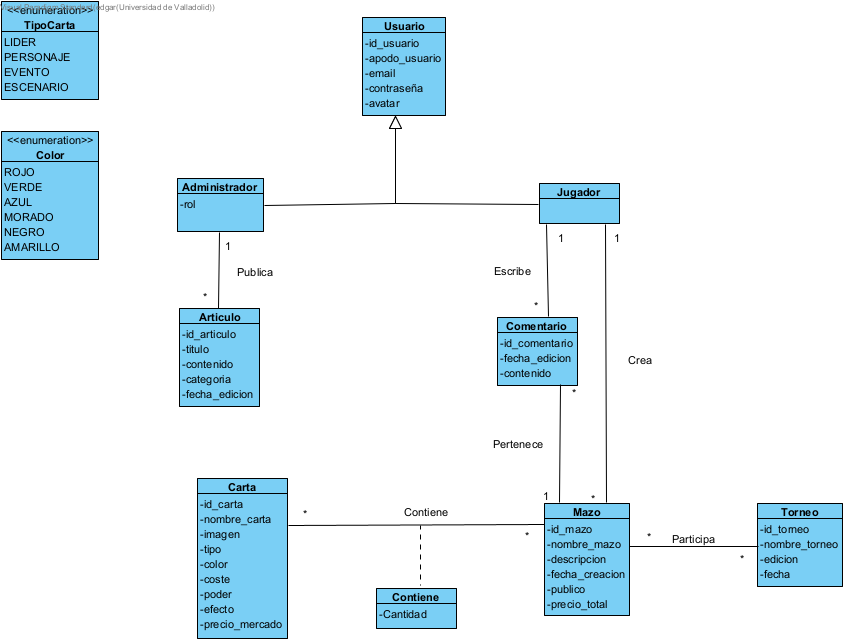
\includegraphics[width=0.9\textwidth]{Recursos/ModeloDominio_Grupo33.png}
		\caption{Diagrama UML del Modelo de Dominio de Card Partner donde definimo los conceptos clave de las reglas de negocio.}
		\label{fig:modelo_dominio}
	\end{figure}
	\newpage
	\subsection{Descripción de las entidades}
	Teniendo la visión general de la aplicación, vamos a ir profundizando en cada una de las entidades.\\
	Emplearemos pequeños diagramas, así como una explicación de sus atributos y las relaciones guardan entre ellas.
	\subsection{Usuarios y roles}
	La clase Usuario representa la información de acceso y autenticación del usuario registrado en la web.
	\begin{figure}[H]
		\centering
		% Columna izquierda: Imagen (45% del ancho de página)
		\begin{minipage}{0.45\textwidth}
			\centering
			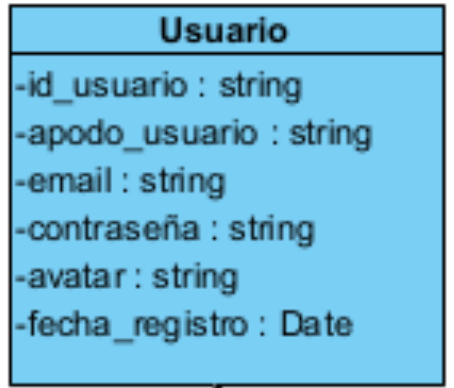
\includegraphics[width=\textwidth]{Recursos/Users&Rols.png}
			\caption{Entidad Usuario}
			\label{fig:User&Rols}
		\end{minipage}
		\hfill % Espacio elástico de separación entre las dos columnas
		% Columna derecha: Lista de atributos (50% del ancho de página)
		\begin{minipage}{0.50\textwidth}
			\textbf{Atributos:}
			\begin{itemize}
				\item \texttt{id\_usuario}: identificador único del sistema.
				\item \texttt{apodo\_usuario}: nombre público elegido por el usuario.
				\item \texttt{email}: cuenta de correo electrónico asociada a la cuenta.
				\item \texttt{contraseña}: credencial del usuario (cifrada).
				\item \texttt{fecha\_registro}: fecha de creación de la cuenta.
				\item \texttt{avatar}: ruta a la imagen pública del perfil del usuario.
				\item \texttt{rol}: tipo de rol que determina los privilegios dentro de la web.\label{key}.
			\end{itemize}
		\end{minipage}
	\end{figure}
	La relaciones que puede tener esta entidad son las siguientes:
	\begin{itemize}
		\item \textbf{Crea(n:m) }con MazoComunidad :  el Usuario puede crear mazos y publicarlos en la web.
		\item \textbf{Guarda(n:m)} con Mazo : el Usuario puede guardar únicamente mazos visibles, es decir, mazos públicos de la comunidad o mazos oficiales/meta. No puede guardar mazos privados de otros usuarios.
		\item \textbf{Escribe (1:n)} con Comentario : el Usuario puede publicar comentarios en los mazos.
		\item \textbf{Valora (n:m)} con Mazo : el Usuario puede dar una valoración en los mazos.
		\item \textbf{Publica(n:m)} con MazoOficial : sólo usuarios con rol ADMIN pueden publicar mazos oficiales/meta.
		\item \textbf{Publica(n:m)} con Articulo : solo usuarios con rol ADMIN pueden publicar artículos (Noticias, Guías o Torneos).
	\end{itemize}
	
	\newpage
	\subsection{Cartas}
	La clase Carta representa la entidad central del TCG y su información estática.\\
	\begin{figure}[H]
		\centering
		% Columna izquierda: Imagen (45% del ancho de página)
		\begin{minipage}{0.45\textwidth}
			\centering
			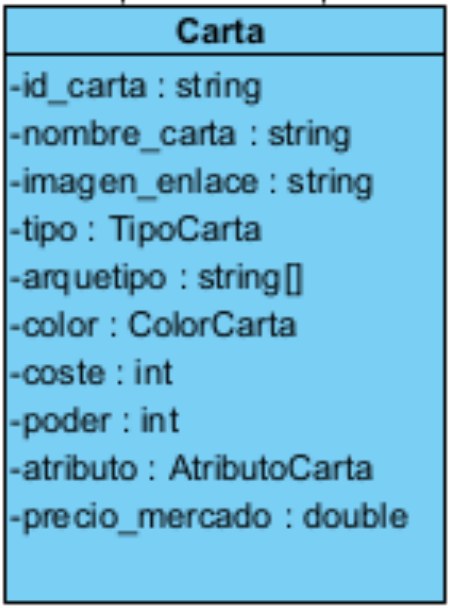
\includegraphics[width=\textwidth]{Recursos/Cards.png}
			\caption{Entidad Carta}
			\label{CartaEntity}
		\end{minipage}
		\hfill % Espacio elástico de separación entre las dos columnas
		% Columna derecha: Lista de atributos (50% del ancho de página)
		\begin{minipage}{0.50\textwidth}
			\textbf{Atributos:}
			\begin{itemize}
				\item id\_carta : código oficial de la carta.
				\item nombre\_carta : nombre de la carta.
				\item imagen\_enlace : ruta a la ilustración de la carta
				\item tipo : clasificación de la carta dentro del TCG de \textit{One Piece}.
				\item arquetipo : familia a la que pertenece la carta (pueden ser varias).
				\item color : clasificación de la carta dentro del TCG de \textit{One Piece}.
				\item coste : puntos necesarios para jugar la carta.
				\item poder : puntos de ataque de la carta.
				\item atributo :tipo de ataque de la carta.
				\item precio\_mercado : valor real de la carta.
			\end{itemize}
		\end{minipage}
	\end{figure}
	Las relaciones que presenta esta entidad son:
	\begin{itemize}
		\item \textbf{Lidera(1:1)} con Mazo : identifica a la única carta líder obligatoria de un mazo.
		\item \textbf{ContieneCarta(n:m)} con Mazo : identifica las cartas que componen un mazo, con cantidad.
	\end{itemize}
	
	\subsection{Artículo}
		\begin{figure}[H]
			\centering
			% Columna izquierda: Imagen (45% del ancho de página)
			\begin{minipage}{0.45\textwidth}
				\centering
				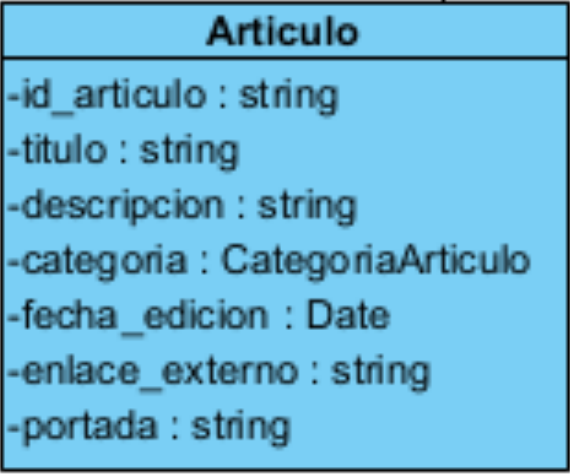
\includegraphics[width=\textwidth]{Recursos/Articulo.png}
				\caption{Contenidos publicados por Usuarios con rol ADMIN.}
				\label{EA}
			\end{minipage}
			\hfill % Espacio elástico de separación entre las dos columnas
			% Columna derecha: Lista de atributos (50% del ancho de página)
			\begin{minipage}{0.50\textwidth}
				\textbf{Atributos:}
				\begin{itemize}
					\item id\_articulo : identificador único.
					\item titulo : titular del artículo.
					\item descripcion : resumen del contenido.
					\item categoria : tipo de artículo (Noticia, Guia, Torneo).
					\item fecha\_creacion : fecha de creación.
					\item fecha\_edicion : fecha de última edición.
					\item enlace\_externo : URL de referencia.
					\item portada : ruta de imagen miniatura
				\end{itemize}
			\end{minipage}
		\end{figure}
	\subsection{Mazos}
	La entidad Mazo representa la estructura común de cualquier mazo publicado en la web.\\
	\begin{figure}[H]
		\centering
		% Columna izquierda: Imagen (45% del ancho de página)
		\begin{minipage}{0.45\textwidth}
			\centering
			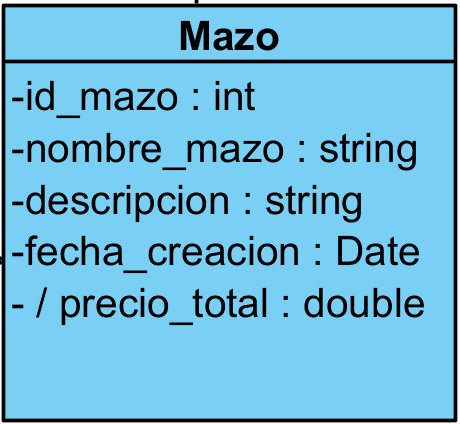
\includegraphics[width=\textwidth]{Recursos/deck.png}
			\caption{Entidad Mazo}
			\label{EntidadMazo}
		\end{minipage}
		\hfill % Espacio elástico de separación entre las dos columnas
		% Columna derecha: Lista de atributos (50% del ancho de página)
		\begin{minipage}{0.50\textwidth}
			\textbf{Atributos:}
			\begin{itemize}
				\item id\_mazo : identificador único del sistema.
				\item nombre\_mazo : título asignado por el creador.
				\item descripcion : texto explicativo del creador.
				\item fecha\_creacion : fecha de creación del mazo.
				\item precio\_total : precio total de todas las cartas que lo componen.
			\end{itemize}
		\end{minipage}
	\end{figure}
	Mazo presenta las siguientes relaciones:
	\begin{itemize}
		\item Usuario: guarda y valora.
		\item Carta: lidera y contieneCarta.
		\item Comentario: pertenece.
	\end{itemize}
		\subsubsection{Mazo de la comunidad}
	
	La clase MazoComunidad representa aquellos mazos que han sido creados por un Usuario (con rol JUGADOR).
	Dicha entidad presenta los siguientes atributos con sus respectivas relaciones \\
	
	\noindent % Evita que la primera columna tenga sangría
	\begin{minipage}[c]{0.48\textwidth}
		\textbf{Atributos:}
		\begin{itemize}
			\item \texttt{es\_publico}: identifica si el usuario creador ha hecho el mazo público o es privado.
		\end{itemize}
	\end{minipage}
	\hfill % Añade un espacio elástico entre las dos columnas
	\begin{minipage}[c]{0.48\textwidth}
		\textbf{Relaciones:}
		\begin{itemize}
			\item \textbf{Usuario:} crea.
		\end{itemize}
	\end{minipage}
	
	\subsubsection{Mazo Oficial}
	
	Esta clase representa aquellos mazos creados por un Usuario con rol ADMIN y contiene datos verificados del entorno competitivo.\\
	\begin{minipage}[t]{0.48\textwidth}
		\textbf{Atributos:}
		\begin{itemize}
			\item \textit{winrate }: porcentaje de victorias del mazo en competiciones oficiales
		\end{itemize}
	\end{minipage}
	\hfill % Añade un espacio elástico entre las dos columnas
	\begin{minipage}[t]{0.48\textwidth}
		\textbf{Relaciones:}
		\begin{itemize}
			\item Usuario: publica
		\end{itemize}
	\end{minipage}
	
	
	\subsubsection{Contiene Carta}
	Esta clase  asociativa  único atributo es \textbf{cantidad } que representa el número de copias de la carta dentro del mazo, ya que es la única información que aporta.
	
	
	
	\subsection{Interacción del usuario}
	En este apartado explicaremos más en profundidad las entidades que representan interacciones directas del usuario en el aspecto social.
	\subsubsection{Comentario}
	Entidad que representa la publicación que un Usuario deja en un Mazo.
	\begin{figure}[H]
		\centering
		% Columna izquierda: Imagen (45% del ancho de página)
		\begin{minipage}{0.45\textwidth}
			\centering
			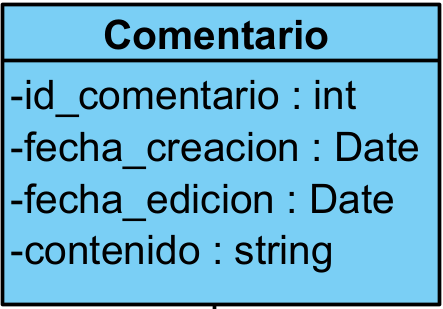
\includegraphics[width=\textwidth]{Recursos/Comentario.png}
			\caption{Entidad comentario.}
			\label{Entidadcomentario}
		\end{minipage}
		\hfill % Espacio elástico de separación entre las dos columnas
		% Columna derecha: Lista de atributos (50% del ancho de página)
		\begin{minipage}{0.50\textwidth}
			\textbf{Atributos:}
			\begin{itemize}
				\item id\_comentario : identificador único.
				\item contenido : texto redactado por el usuario.
				\item fecha\_creacion : fecha de creación del comentario.
				\item fecha\_edicion : fecha de última edición.
			\end{itemize}
		\end{minipage}
	\end{figure}
	Esta entidad sólo tiene una relación con la entidad mazo, la cual es de pertenencia.
	\newpage
	\subsubsection{Valoración}
	Clase asociativa entre Usuario y Mazo.\\
	\begin{figure}[H]
		\centering
		% Columna izquierda: Imagen (45% del ancho de página)
		\begin{minipage}{0.45\textwidth}
			\centering
			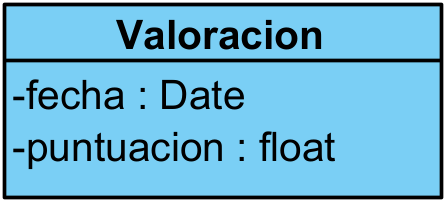
\includegraphics[width=\textwidth]{Recursos/Valoración.png}
			\caption{Entidad valoración.}
			\label{fn}
		\end{minipage}
		\hfill % Espacio elástico de separación entre las dos columnas
		% Columna derecha: Lista de atributos (50% del ancho de página)
		\begin{minipage}{0.50\textwidth}
			\textbf{Atributos:}
			\begin{itemize}
				\item fecha\_valoracion : fecha de la valoración.
				\item puntuacion : valor numérico asignado.
			\end{itemize}
		\end{minipage}
	\end{figure}
	\subsubsection{Whislist}
	Esta entidad actúa como una clase asociativa que representa la interacción de guardado entre un Jugador y una carta.
	\begin{figure}[H]
		\centering
		% Columna izquierda: Imagen (45% del ancho de página)
		\begin{minipage}{0.45\textwidth}
			\centering
			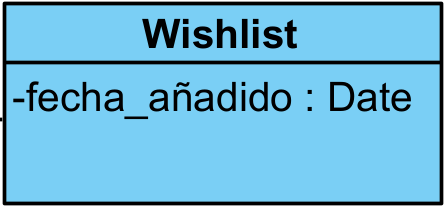
\includegraphics[width=\textwidth]{Recursos/Wishlist.png}
			\caption{Entidad \textit{whishlist}}
			\label{EW}
		\end{minipage}
		\hfill % Espacio elástico de separación entre las dos columnas
		% Columna derecha: Lista de atributos (50% del ancho de página)
		\begin{minipage}{0.50\textwidth}
			\textbf{Atributos:}
			\begin{itemize}
				\item fecha\_añadido: 
			\end{itemize}
		\end{minipage}
	\end{figure}
	\textit{Whishlist} presenta las siguientes relaciones:
	\begin{itemize}
		\item Usuario: el cual ha de tener una sesión inciada en nuestra aplicación
		\item Carta: la entidad que el usuario quiere añadir a su lista de deseados.
	\end{itemize}
	\newpage
	\section{Desarrollo de CardPartner}	
	Llegados a este punto, ya tenemos establecidos unos planos sólidos sobre cómo ha de ser nuestra aplicación web, por lo que a partir de este punto documentaremos las diferentes etapas en el desarrollo del proyecto, partiendo desde el bocetaje incial, pasando por el desarrollo del \textit{frontent} estático, la posterior incorporación del \textit{backend} y por último la funcionalidad definitiva para hacer pasar a \textit{Card Partner} de una idea a una web funcional.
	\subsection{Primera versión del bocetaje}
	En la primera fase hemos realizado unos esquemas a mano alzada sobre el aspecto y funcionalidades de la web (para consultar los bocetos con más detalle puesto que \underline{no} son imágenes vectorizadas diríjase a \href{https://uvaes-my.sharepoint.com/:b:/g/personal/alvaro_lopez_primo_estudiantes_uva_es/IQDlwgU7uvVIR4IvbixZFawhAXxjL6flgH43ePd4Q4bNtks?e=ghkMdm}{este enlace}).
	\begin{figure}[H]
		\centering
		\begin{subfigure}{0.45\textwidth}
			\centering
			\includegraphics[width=\textwidth]{Recursos/inicio.png}
			\caption{Vista inicial de la página con la opción de \textit{login} y con una cuenta ya creada donde se verán unas breves noticias sobre el \textit{TCG}, un apartado de las normas básicas del juego y una sección de mazos recomendados para principiantes.}
			\label{InicioPagina}
		\end{subfigure}
		\hfill 
		\begin{subfigure}{0.45\textwidth}
			\centering
			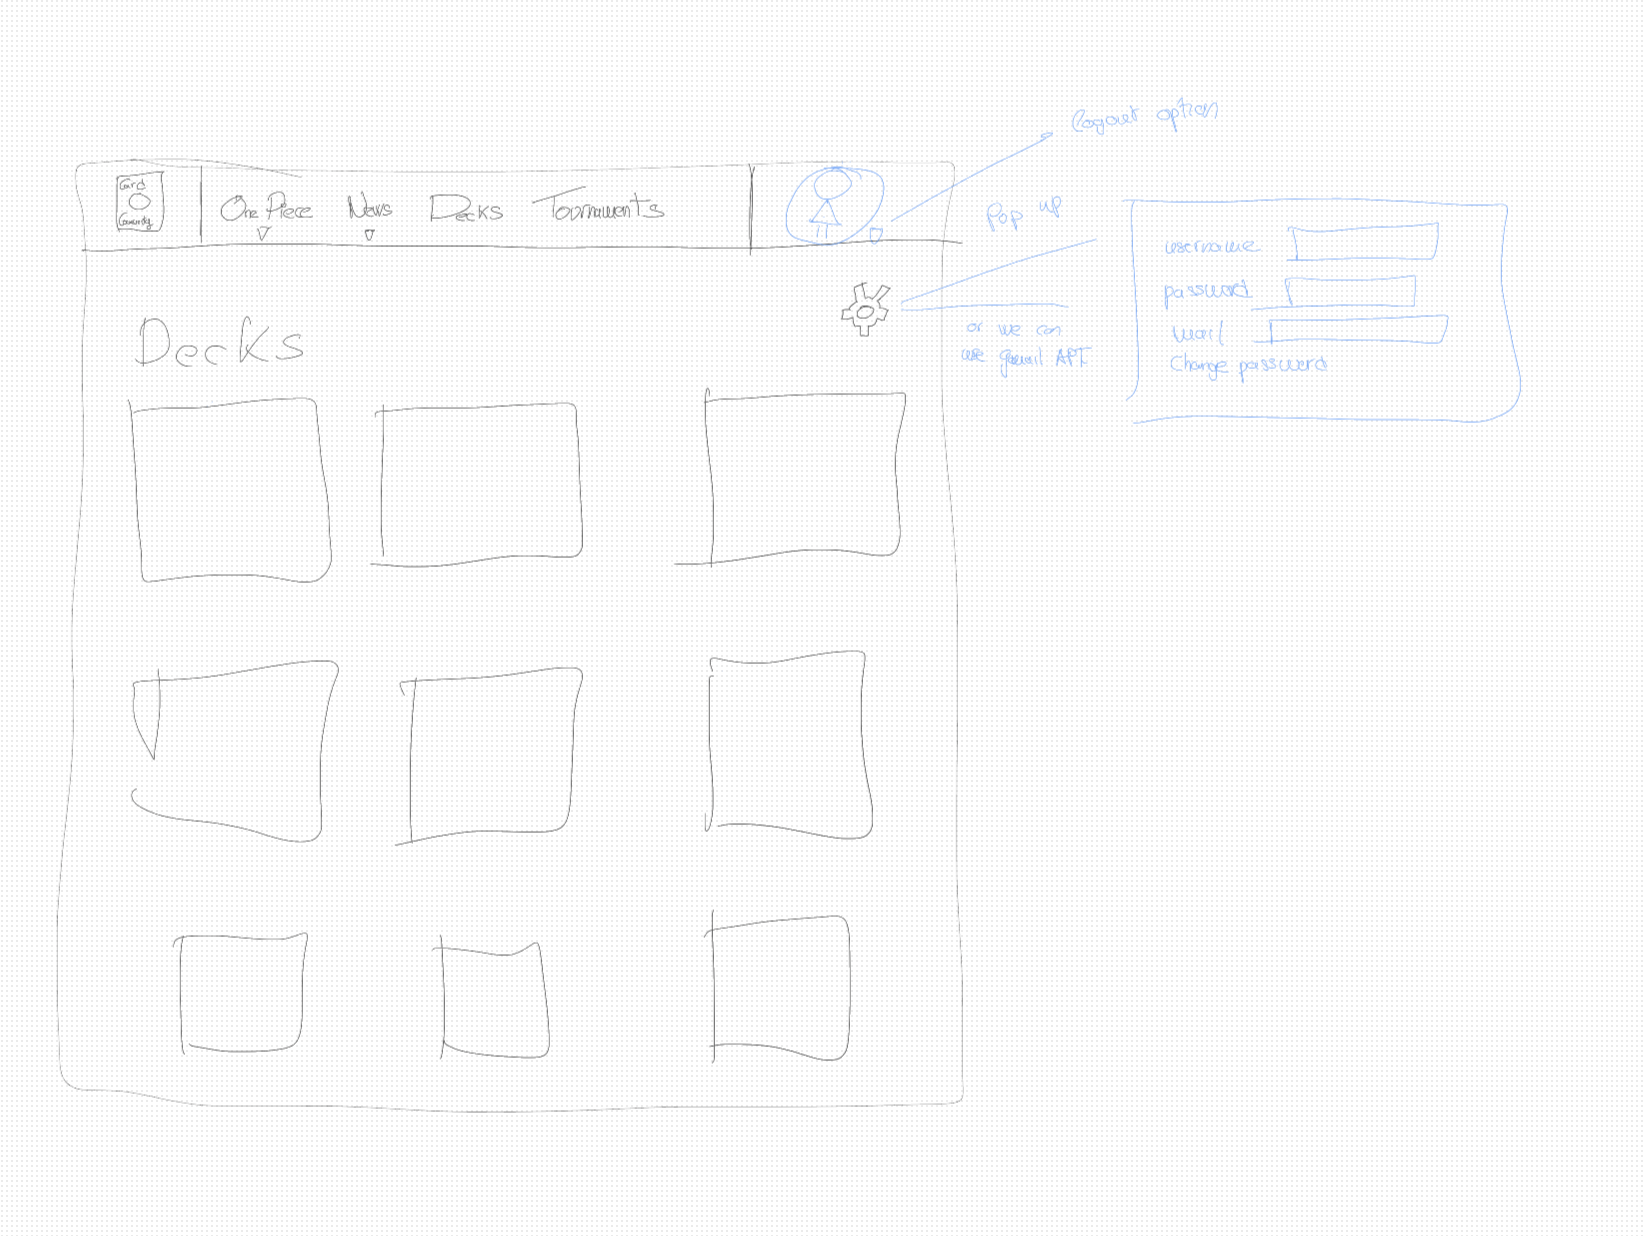
\includegraphics[width=\textwidth]{Recursos/user.png}
			\caption{Vista del usuario donde podrá ver los mazos que ha creado y una rueda de opción donde poder realizar diferentes funciones sobre su perfil (cambiar contraseña)}
			\label{UserView}
		\end{subfigure}
	\end{figure}
	\begin{figure}[H]
		\centering
		\begin{subfigure}{0.45\textwidth}
			\centering
			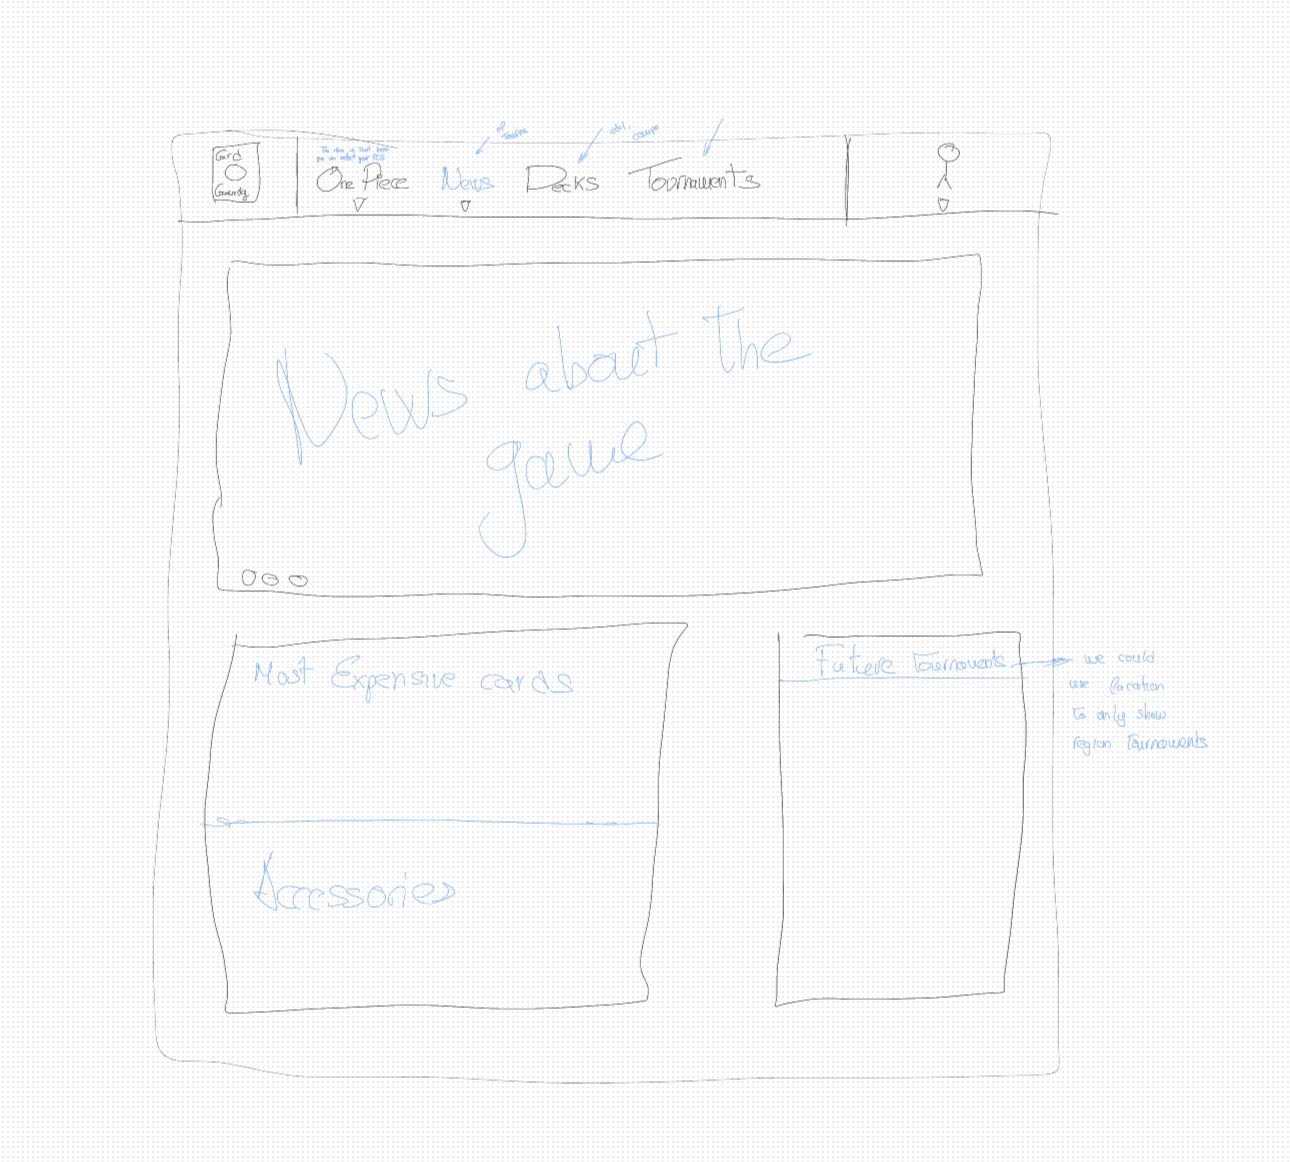
\includegraphics[width=\textwidth]{Recursos/noticias.png}
			\caption{Vista del apartado de noticias. En ella observamos novedades del \textit{TCG} así como una selección de cartas más caras y de accesorios típicos para dichos juegos así como una lista de los futuros torneos.}
			\label{Notcias}
		\end{subfigure}
		\hfill 
		\begin{subfigure}{0.45\textwidth}
			\centering
			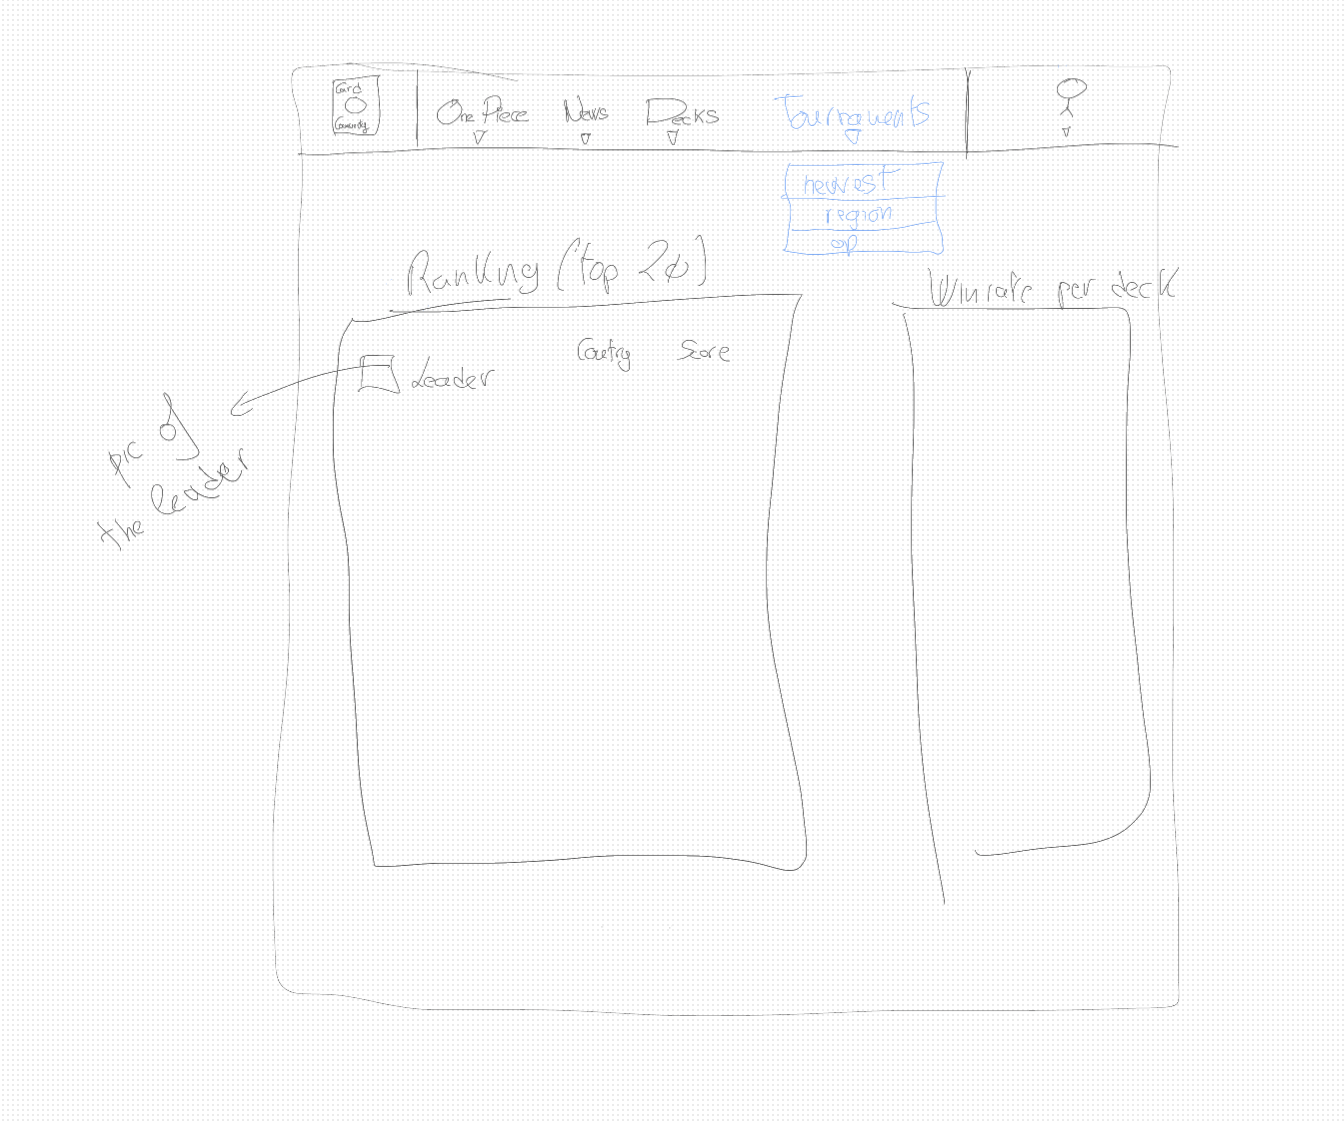
\includegraphics[width=\textwidth]{Recursos/tournaments.png}
			\caption{Vista de la pestaña de torneos. Incluye un ranking global de mazos y un porcentaje de victoria de cada líder.}
			\label{ftr}
		\end{subfigure}
	\end{figure}
	\begin{figure}[H]
		\centering
		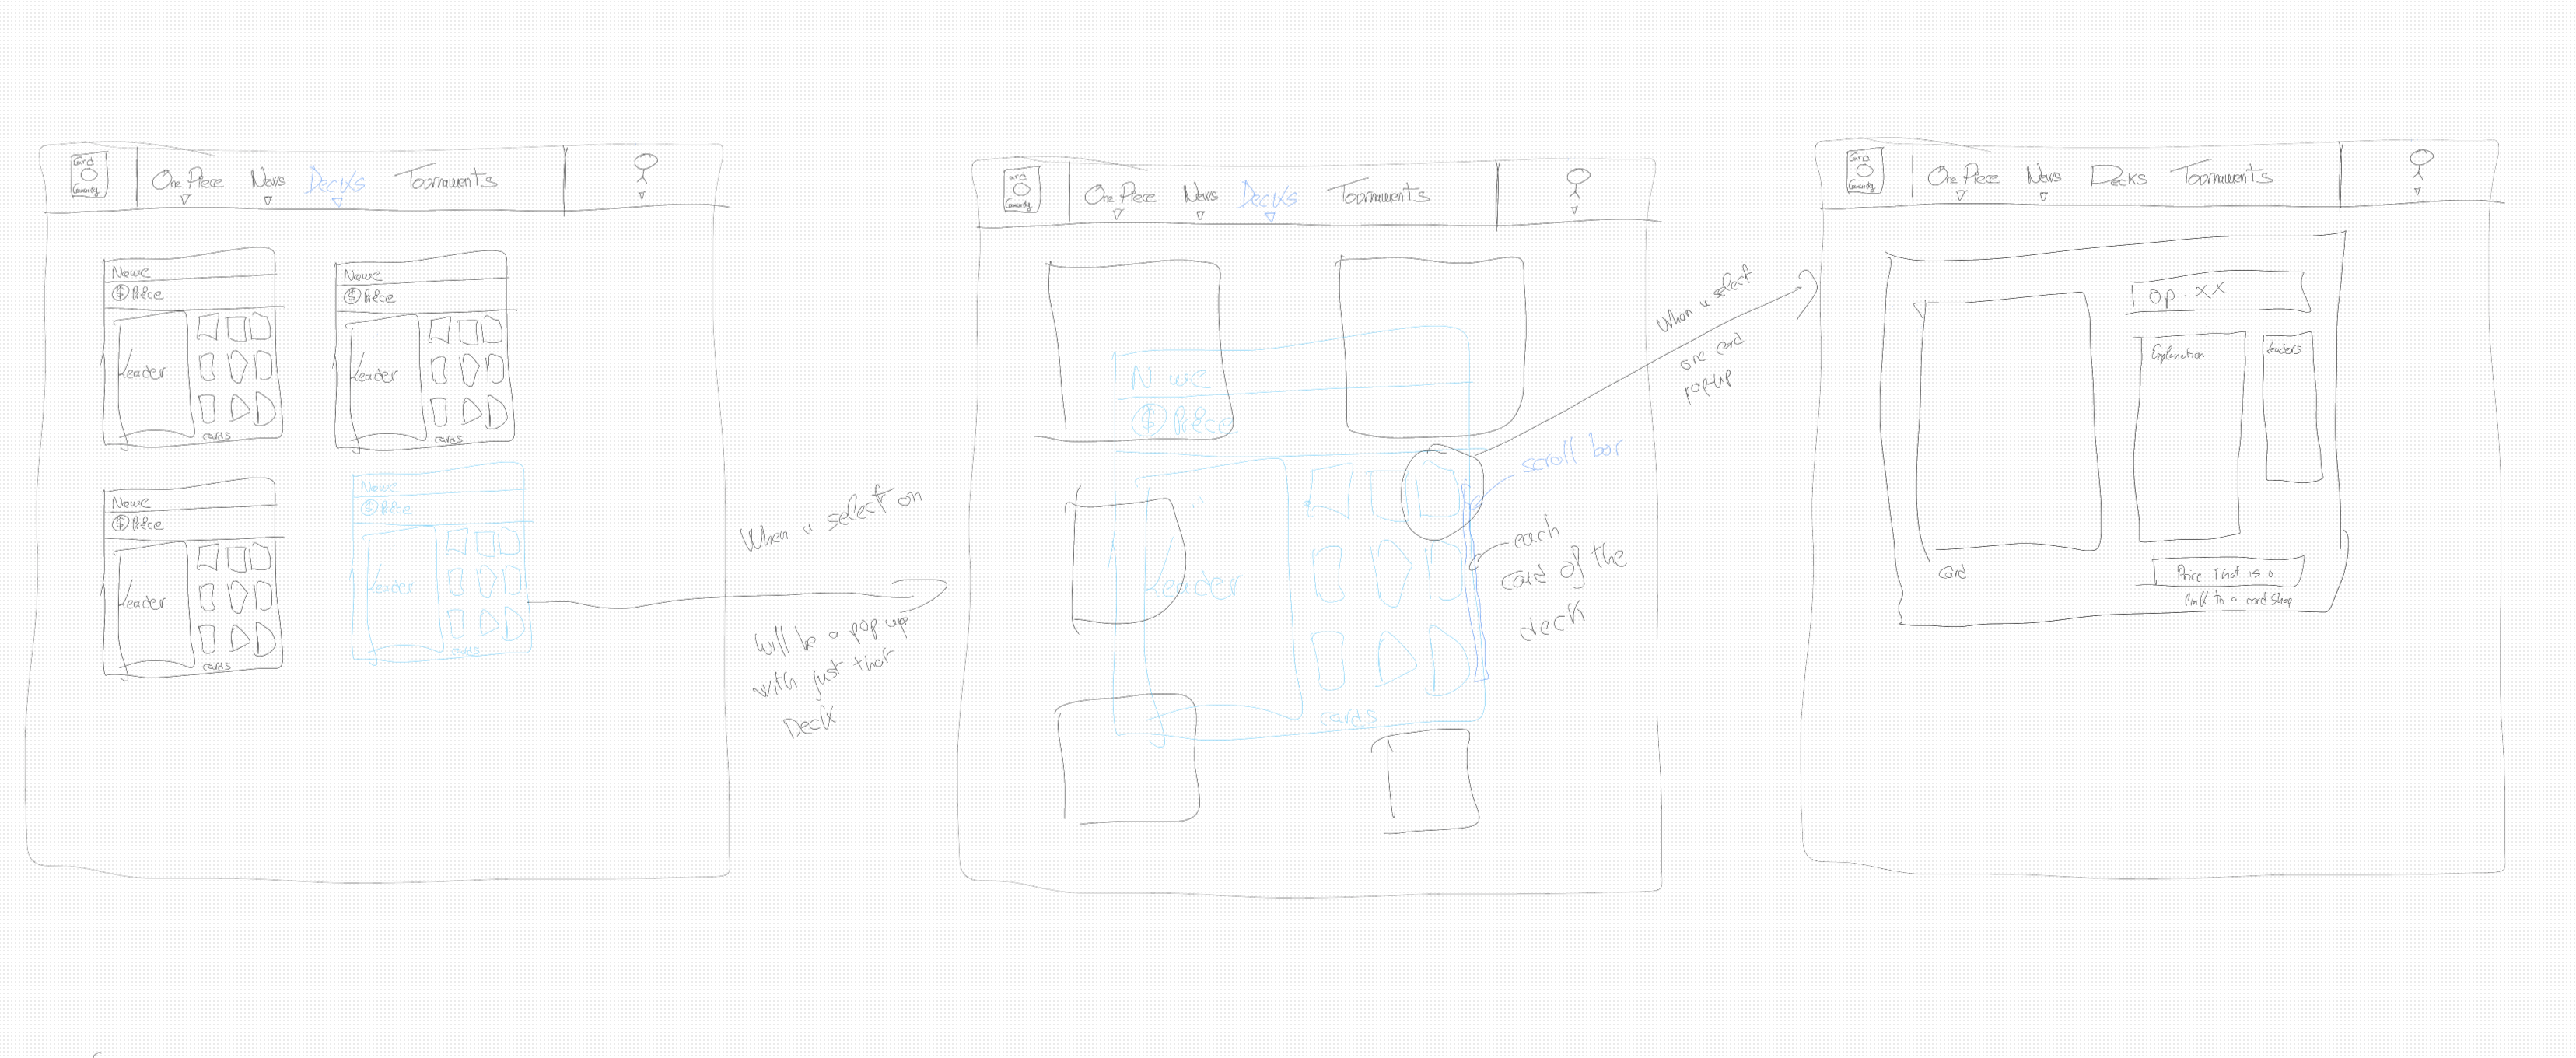
\includegraphics[width=0.85\textwidth]{Recursos/decks.png}
		\caption{Vista del apartado Deck. Se muestran los diferentes mazos creados por la comunidad, con la opción de seleccionar sobre ellos y poder consultar todas las cartas. Además se incluye una opción a las personas con una cuenta en la web de comentar en los mazos}
	\end{figure}
	
	
	\subsection{Segunda iteración sobre los bocetos}
	Una vez que todos hemos dado el visto bueno a los bocetos a mano alzada, decidimos emplear la herramienta \textit{draw.io} para realizar unos bocetos más limpios y organizados (para consultar las imágenes con más detalle, diríjase a \href{https://drive.google.com/file/d/1g8FwPydQRjYX_IET-vt37nWVM2JCpji7/view}{este enlace})\\
	Esta mejora en la organización se debe a que hemos dividido los bocetos en módulos, los cuales se pueden consultar en la siguiente tabla
	\begin{table}[H]
		\centering
		\renewcommand{\arraystretch}{1.5}
		\begin{tabularx}{\textwidth}{|>{\raggedright\arraybackslash\bfseries}p{3cm}|>{\raggedright\arraybackslash}X|}
			\hline
			Módulo principal & Funcionalidades y características \\
			\hline
			Comunidad & Acceso a guías de aprendizaje, noticias sobre el juego y seguimiento de torneos. \\
			\hline
			Mazos & Consulta del meta actual con estadísticas, acceso a mazos de la comunidad (con filtros, valoraciones y comentarios) y una herramienta interactiva para la creación de mazos propios. \\
			\hline
			Cartas & Catálogo completo con listado de cartas, filtros de búsqueda avanzados, estadísticas detalladas y precios de mercado. \\
			\hline
			Usuario & Gestión integral de la cuenta: inicio de sesión, registro, edición de información personal (correo, contraseña) y un panel de control para administrar mazos (creados, publicados y guardados) e interacciones sociales. \\
			\hline
		\end{tabularx}
		\caption{Descripción general de los módulos y funcionalidades de la plataforma.}
		\label{tmodulos_app}
	\end{table}
	%\newpage
	En la siguiente página podemos observar los nuevos bocetos, más estructurados y profesionales  realizados con la herramienta \textit{draw.io}. 
	\begin{landscape}
		\thispagestyle{empty} 
		\begin{figure}[p]
			\centering
			% El truco está en esta línea:
			\makebox[\linewidth][c]{%
				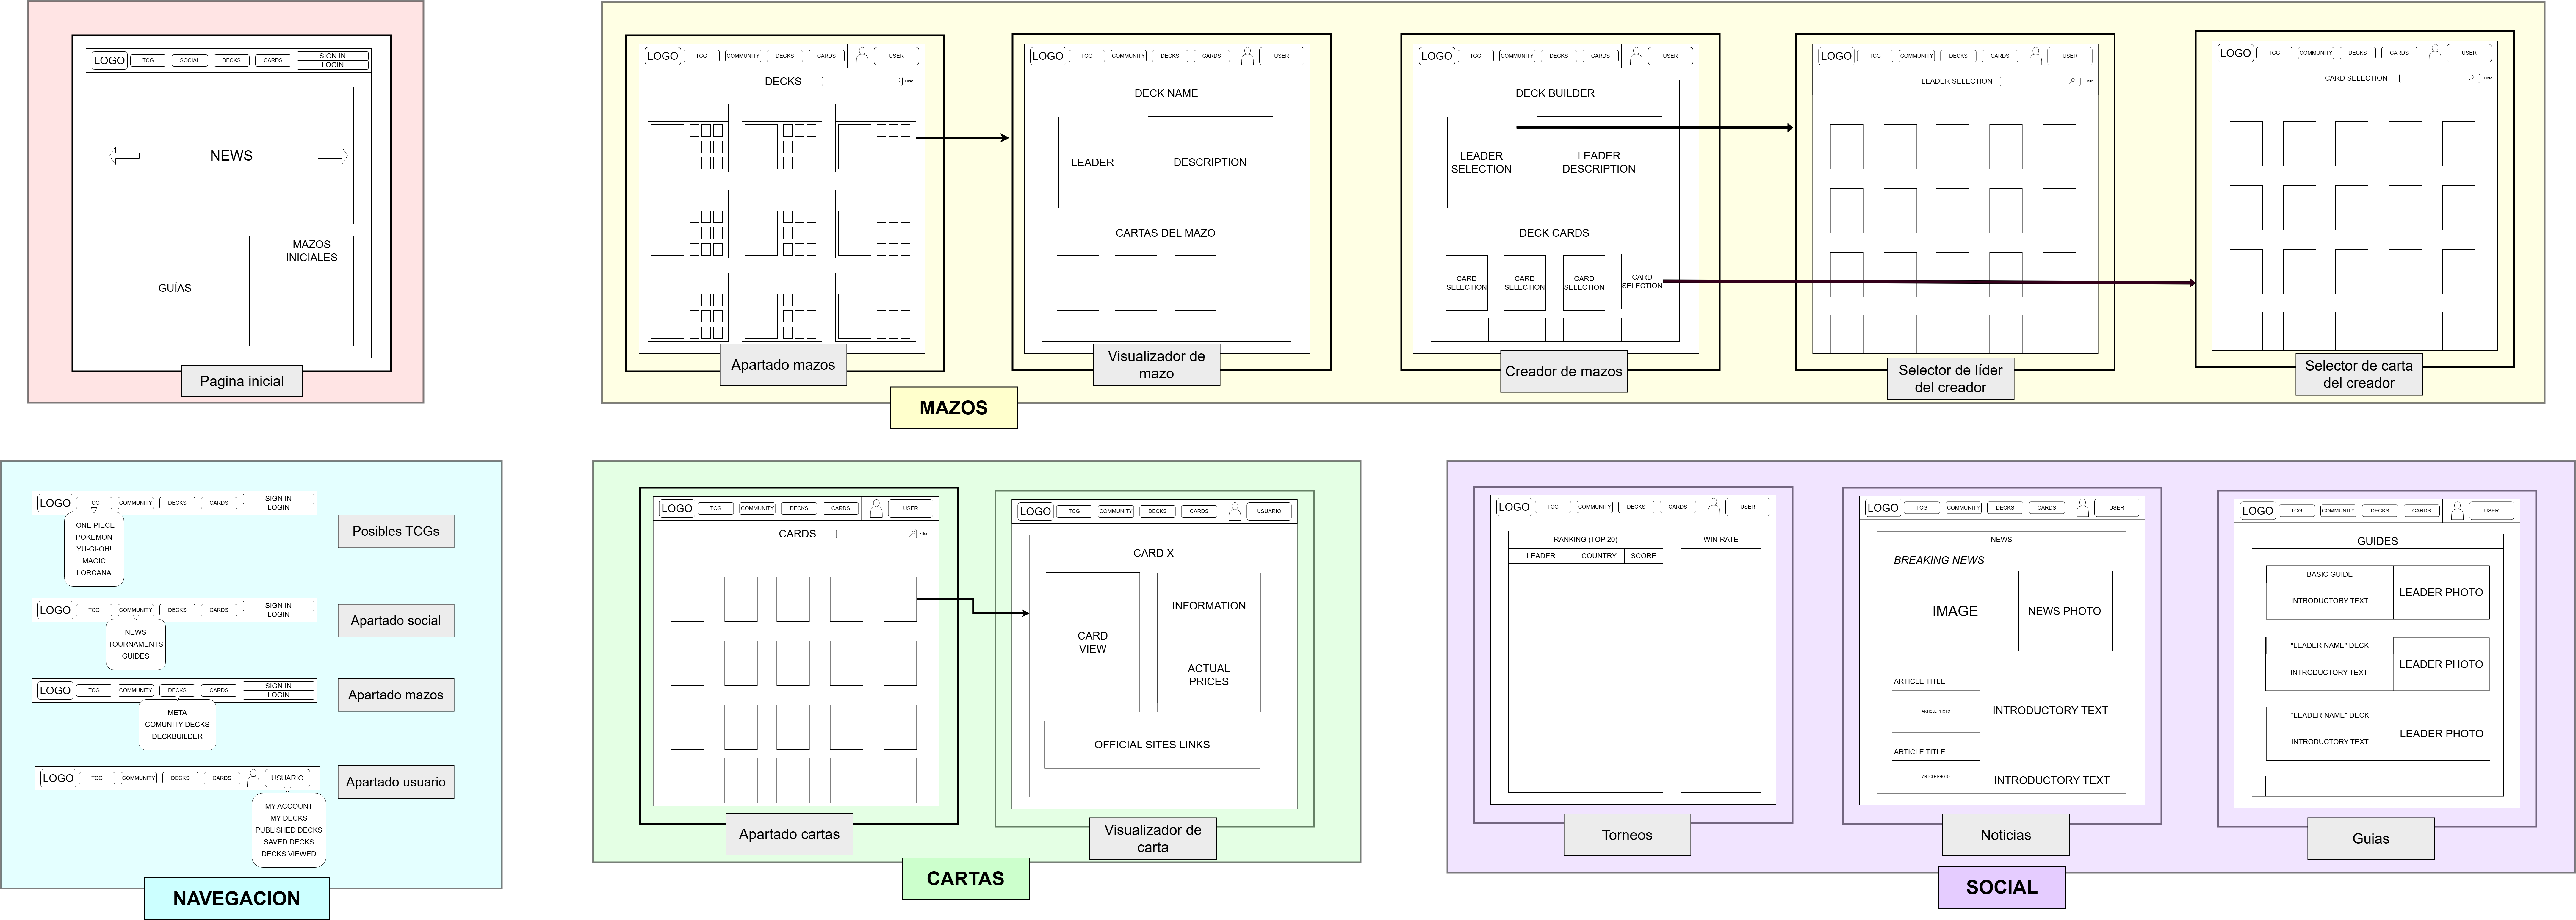
\includegraphics[width=1.18\linewidth, height=1.18\textheight, keepaspectratio]{Recursos/Bocetos2v2.png}
			}
			\caption{Vista completa de los bocetos de Draw.io}
		\end{figure}
	\end{landscape}
	
	%\begin{figure}[H]
	%	\centering
	%	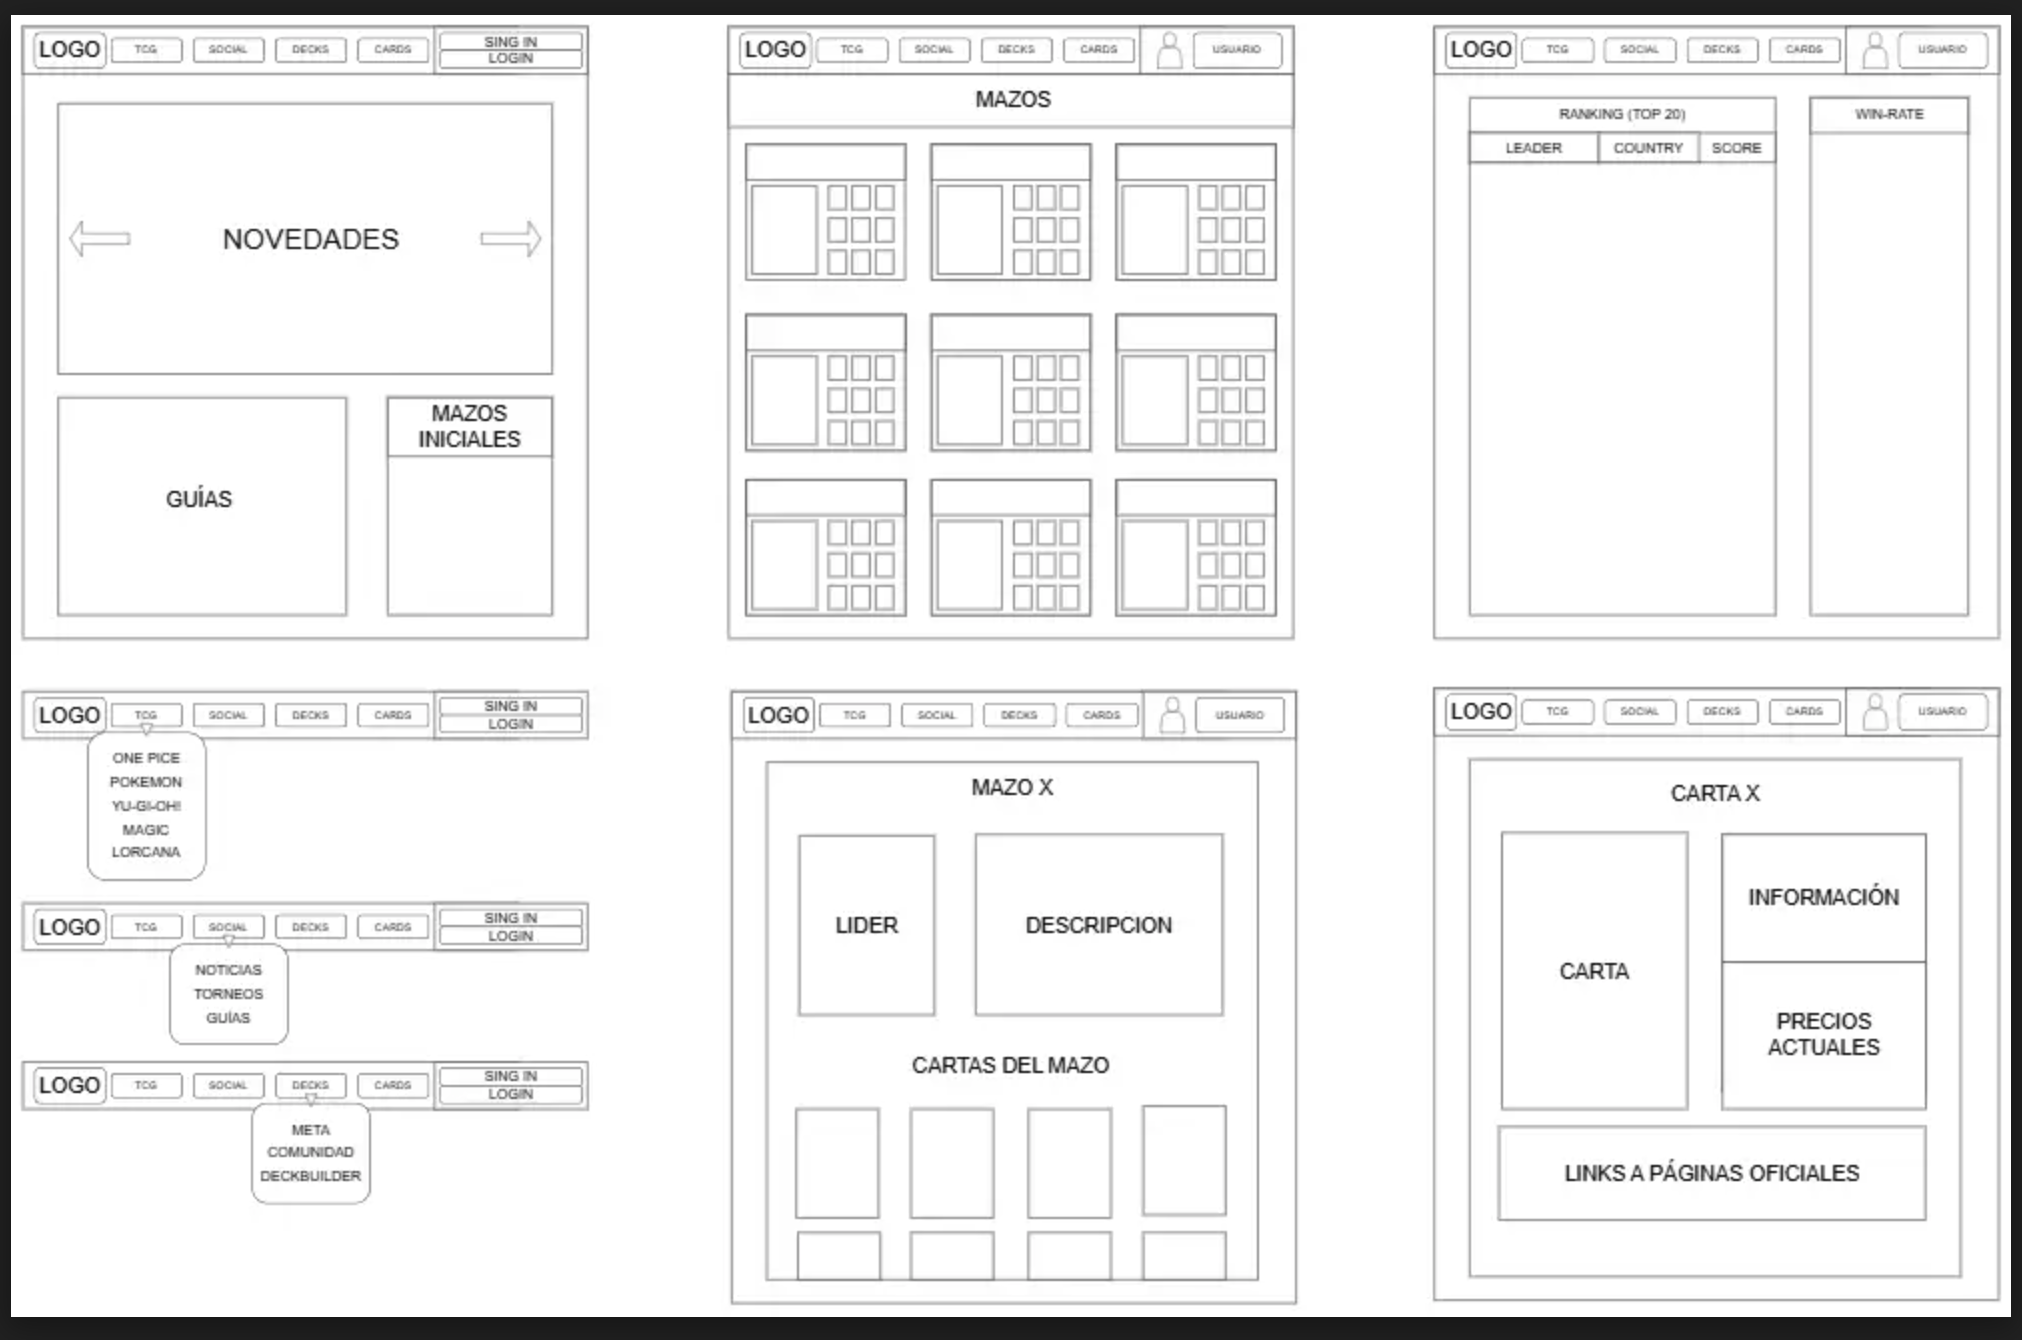
\includegraphics[width=0.85\textwidth]{Recursos/Bocetos2.png}
	%	\caption{\textbf{Boceto limpio con todas las vistas}}
	%\end{figure}
	
	\subsubsection{Vista inicial}
	\begin{figure}[H]
		\centering
		% Columna izquierda: Imagen (45% del ancho de página)
		\begin{minipage}{0.5\textwidth}
			\centering
			\centering
			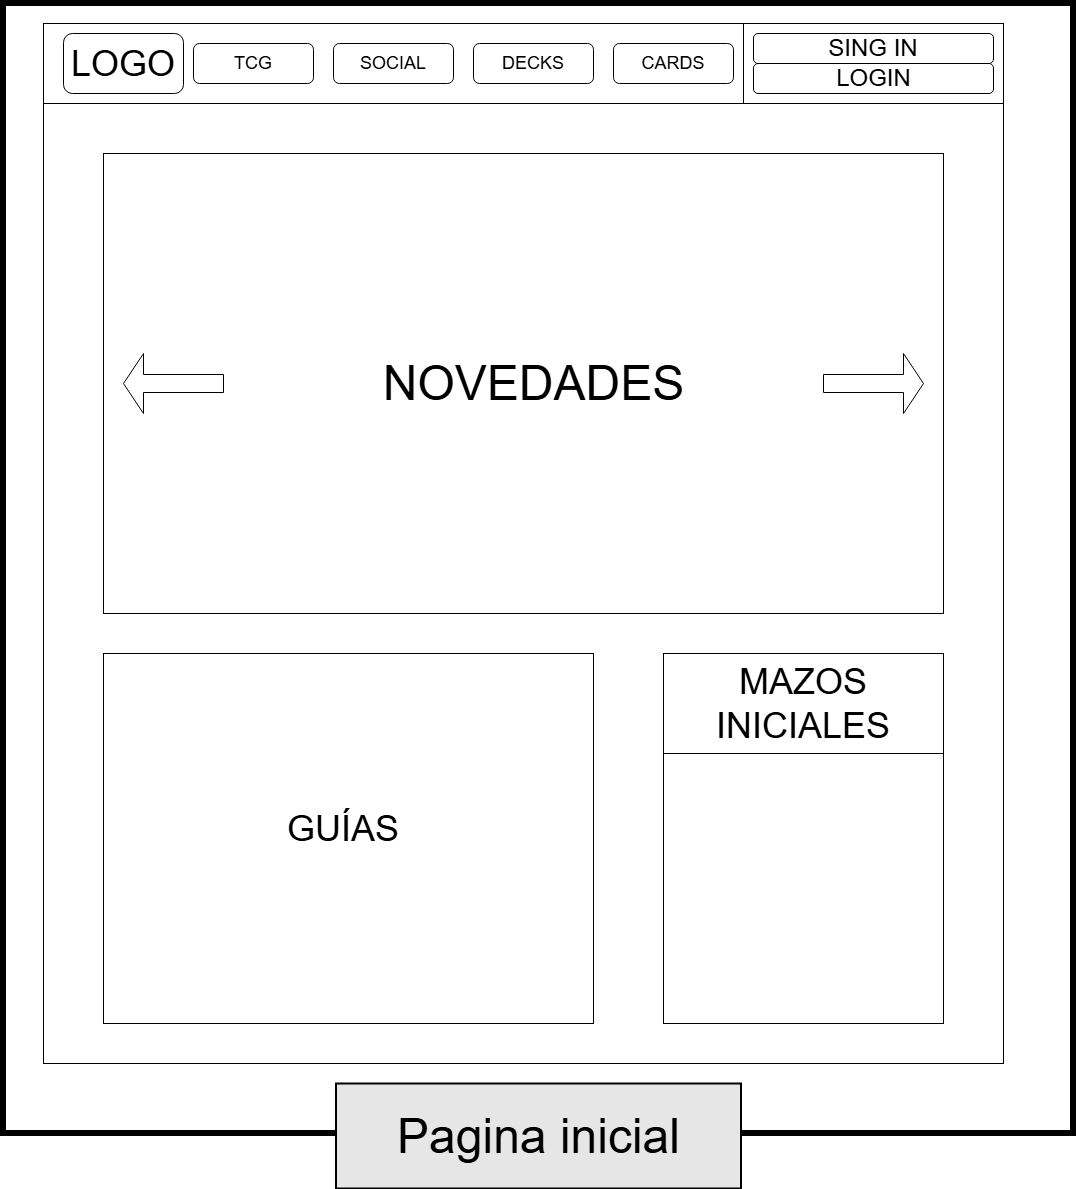
\includegraphics[width=0.85\textwidth]{Recursos/Boceto2_Inicio.png}
			\caption{\textbf{Boceto de la página de Inicio}}
		\end{minipage}
		\hfill % Espacio elástico de separación entre las dos columnas
		% Columna derecha: Lista de atributos (50% del ancho de página)
		\begin{minipage}{0.45\textwidth}
			Observamos que la página inicial se compone de dos elementos clave, la barra de navegación (explicada en la siguiente captura) y los contenidos más relevantes. Enfocándonos en los contenidos relevantes, hemos planteado que se incluya un subapartado de novedades (nuevas expansiones disponibles, información destacada sobre torneos, noticias relacionadas con el \textit{TCG}, etc.), un subapartado con las guías para principiantes y un subapartado con los mejores mazos con los que comenzar a jugar.
		\end{minipage}
	\end{figure}
	
	\subsubsection{Barra de navegación de la página}
	\begin{figure}[H]
		\centering
		% Columna izquierda: Imagen (45% del ancho de página)
		\begin{minipage}{0.5\textwidth}
			\centering
			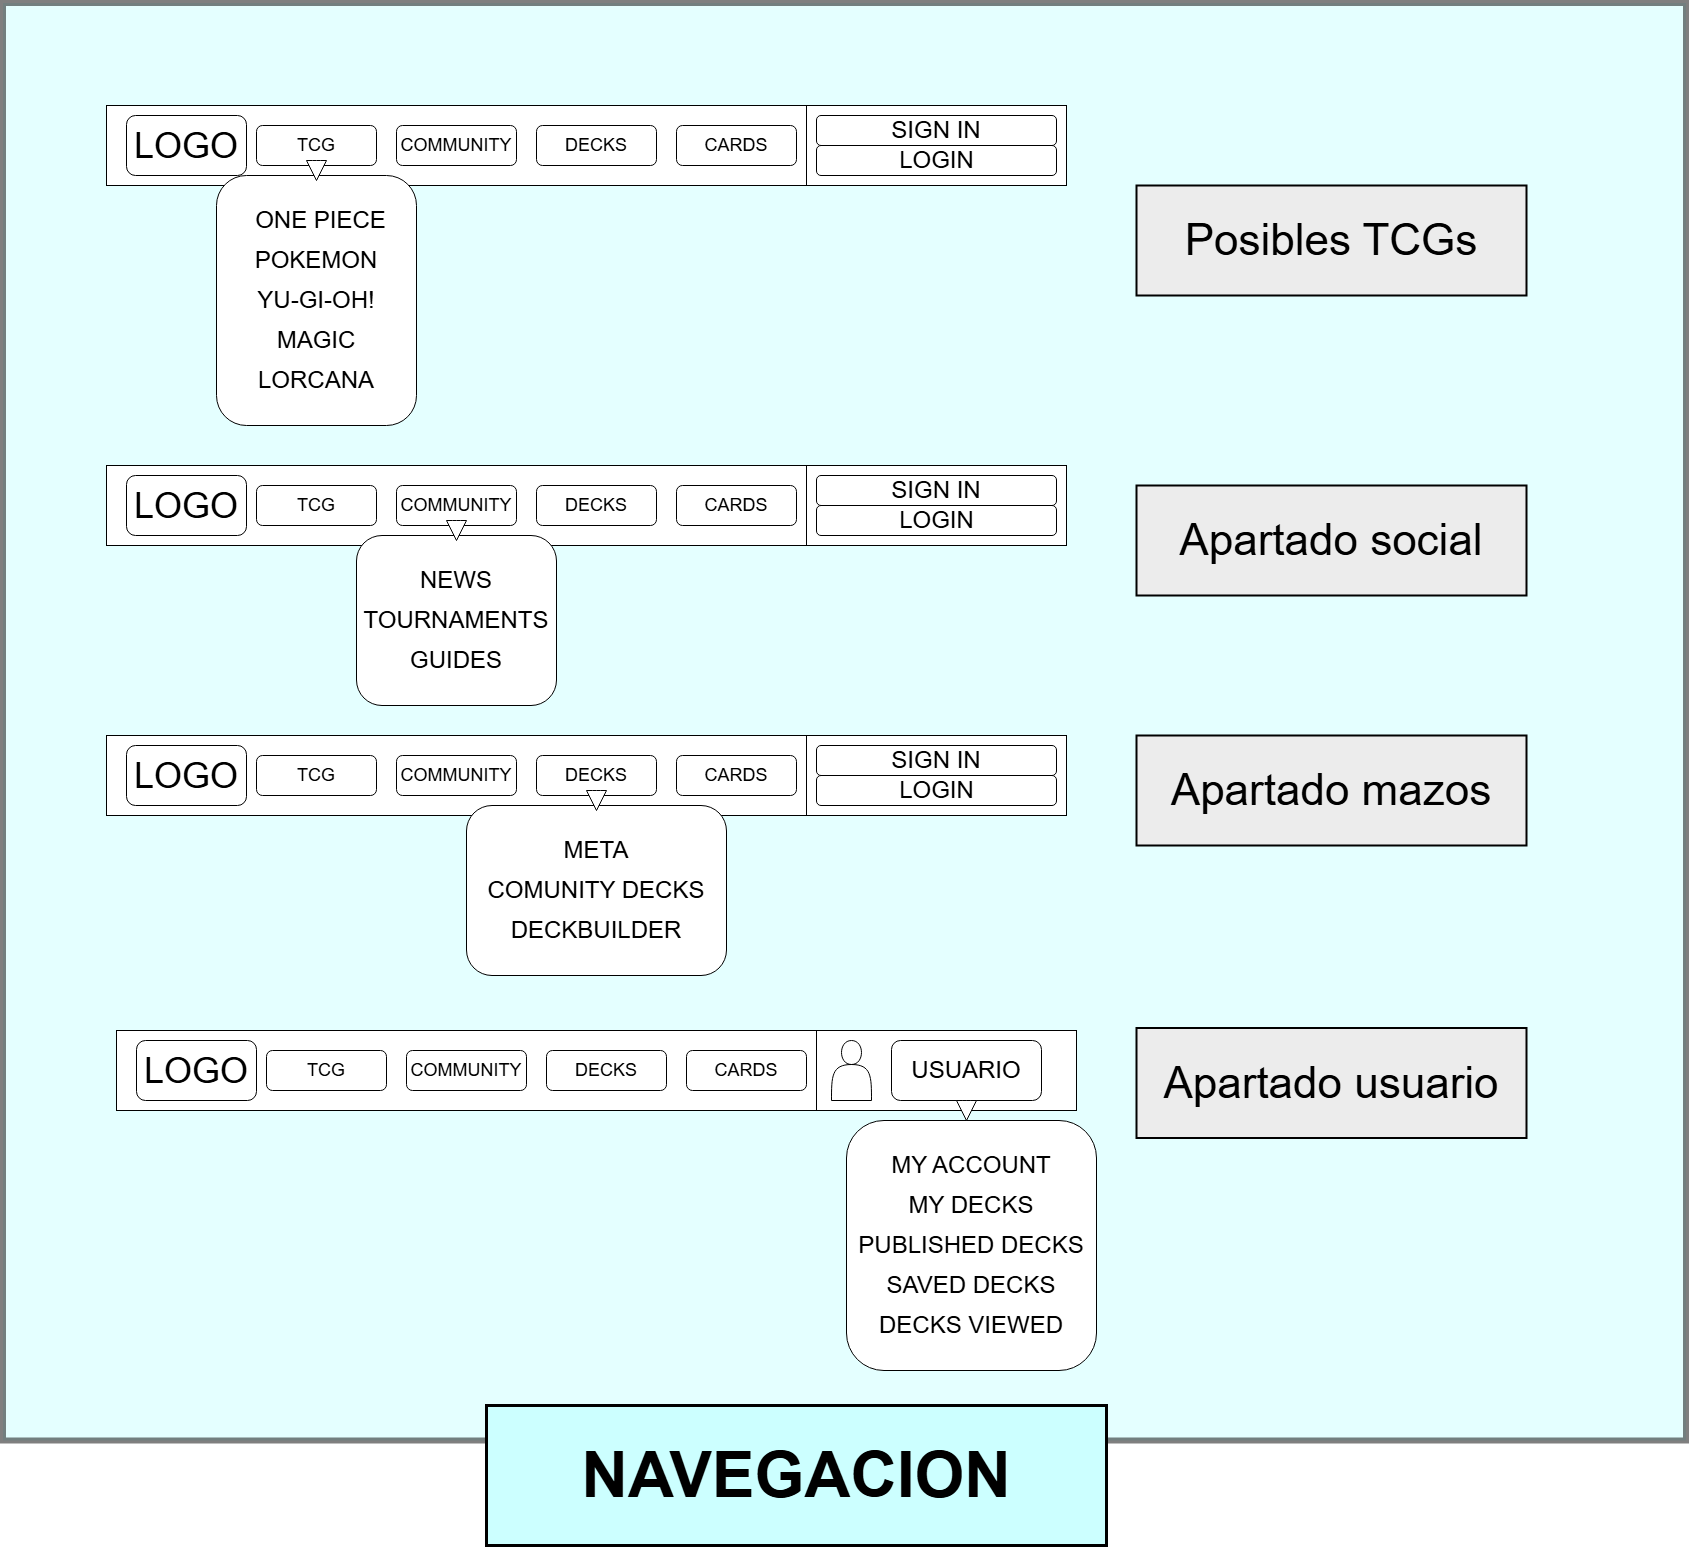
\includegraphics[width=0.85\textwidth]{Recursos/Boceto2_Navegacion.png}
			\caption{\textbf{Boceto de la barra de navegación}}
		\end{minipage}
		\hfill % Espacio elástico de separación entre las dos columnas
		% Columna derecha: Lista de atributos (50% del ancho de página)
		\begin{minipage}{0.45\textwidth}
			La barra de navegación es el motor de navegabilidad principal de nuestra aplicación web, ya que permite al usuario desplazarse por las diferentes funcionalidades de la web de una manera simple y organizada, donde la información está categorizada por menús generales que contienen las diferentes vistas con las que está relacionada, permitiendo al usuario llegar a la opción deseada con un leve movimiento del ratón.\\
			Para hablar sobre la navegación podemos dividir la barra en dos secciones: sección del juego y sección del usuario. \\
			
			En la sección de \textbf{juego} observamos, de izquierda a derecha, las siguientes categorías: \textit{TCG}, \textit{Community} (comunidad), \textit{Decks} (mazos) y \textit{Cards} (cartas). \\La categoría \textbf{TCG} hace referencia a los principales juegos que existen (como hemos mencionado anteriormente nos enfocaremos en el juego basado en \textit{One Piece}). En comunidad podemos acceder a las vistas relacionadas con la interacción del usuario en la comunidad: noticias, torneos y guías de usuario. La siguiente categoría, \textbf{Decks}, incluye todo aquello relacionado con mazos: Mazos empleados en el \textit{META}, mazos creados por la comunidad y el creador de mazos del usuario. Por último nos encontramos con la categoría \textit{Cards}, la cual nos lleva a la lista completa de cartas existentes. \\
		\end{minipage}
	\end{figure}
	
	Por otro lado nos encontramos la sección del \textbf{usuario}. Inicialmente vemos dos opciones, la opción de \textit{Crear cuenta}, pensada para miembros sin un perfil registrado en nuestra web; y la opción de \textit{Iniciar sesión}, enfocada a que los miembros puedan entrar a sus respectivas cuentas. Una vez iniciada la sesión cambiarán los botones a uno que despliegue un menú con las diferentes opciones: Mi cuenta, mazos creados, mazos publicados, mazos guardados e interacciones.
	
	\subsubsection{Comunidad}
	
	\begin{figure}[H]
		\centering
		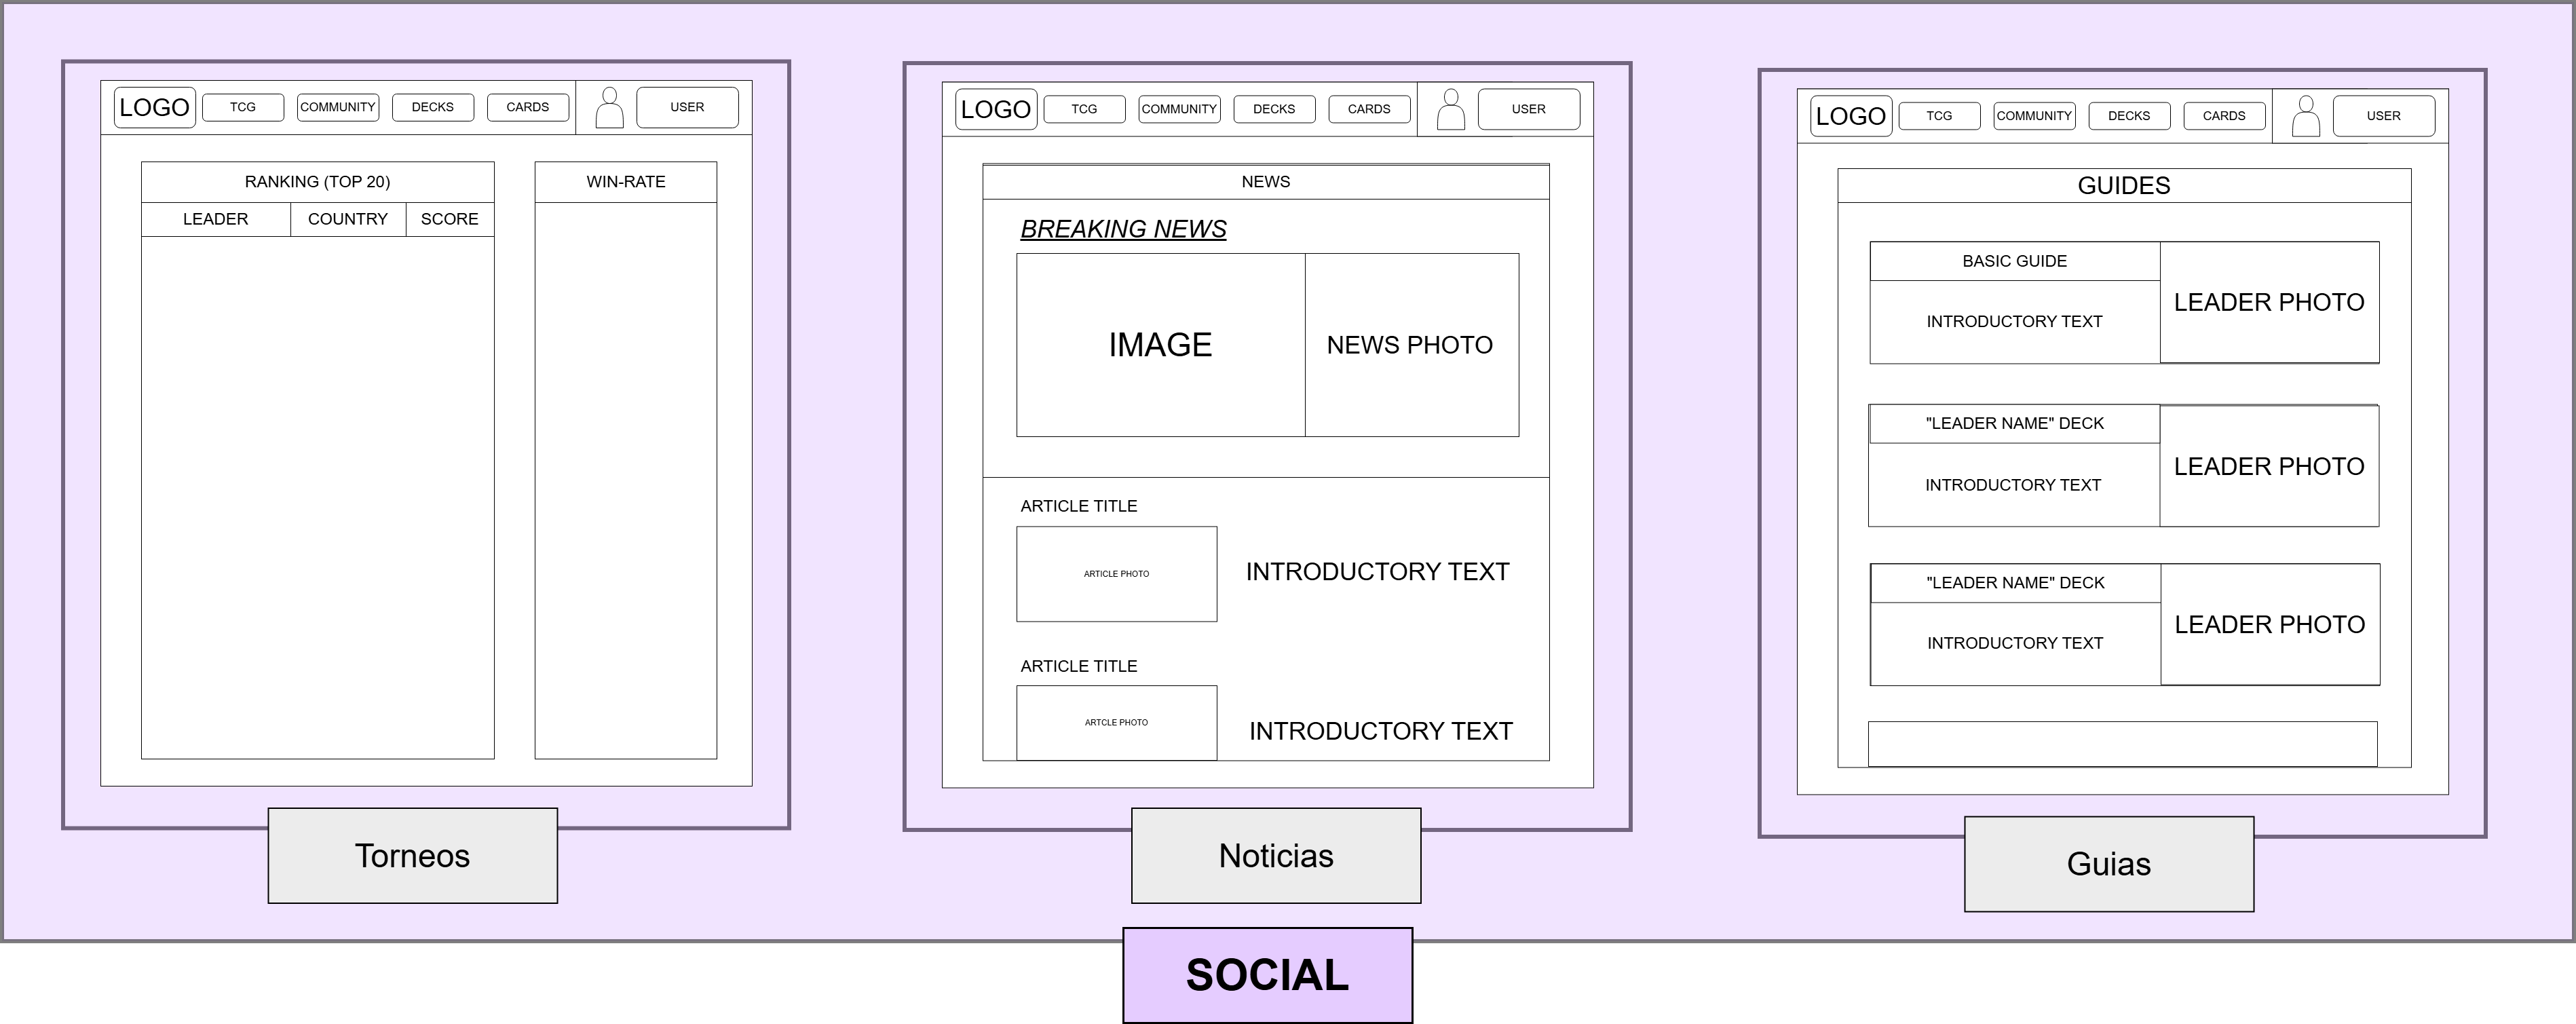
\includegraphics[width=0.85\textwidth]{Recursos/Boceto2_Social.png}
		\caption{\textbf{Boceto de las pestañas de la comunidad}}
	\end{figure}
	
	Nos adentramos ahora en la sección de comunidad. Esta estará dividida en tres opciones diferentes: torneos, noticias y guías. \\
	
	En el apartado de torneos tendremos una lista con los diferentes eventos que hay (torneos pasados o futuros). \\Al seleccionar un torneo entramos en el visualizador del torneo, el cual se compone de dos listas, la lista de \textit{Ranking}, que muestra las posiciones de los diferentes mazos participantes en orden de su desempeño en la competición; y el apartado de \textit{Win-rate}, donde nos informará con una lista sobre el porcentaje de victorias que ha tenido cada carta líder participante. \\
	
	Pasamos ahora a las noticias. En esta vista nos encontramos con una lista que incluye las noticias relacionadas con el mundo del \textit{TCG}. En la parte superior veremos las noticias con mayor relevancia, y en la parte inferior el listado con todas las noticias ordenadas por fecha más reciente. \\Cada noticia incluye un títular, una imagen y una pequeña sinopsis. Al hacer click en ella veremos la noticia elegida en su totalidad. \\
	
	Muy similar al apartado anterior, el de guias se compone de una lista con todas las guias publicadas hasta el momento. Cada noticia tiene un nombre, una breve explicación y una imagen relacionada con ella. Al seleccionar una guia se nos abrirá un visualizador completo de la guia, con sus instrucciones, imagenes explicativas e incluso vídeos informativos.
	
	\subsubsection{Mazos}
	
	\begin{figure}[H]
		\centering
		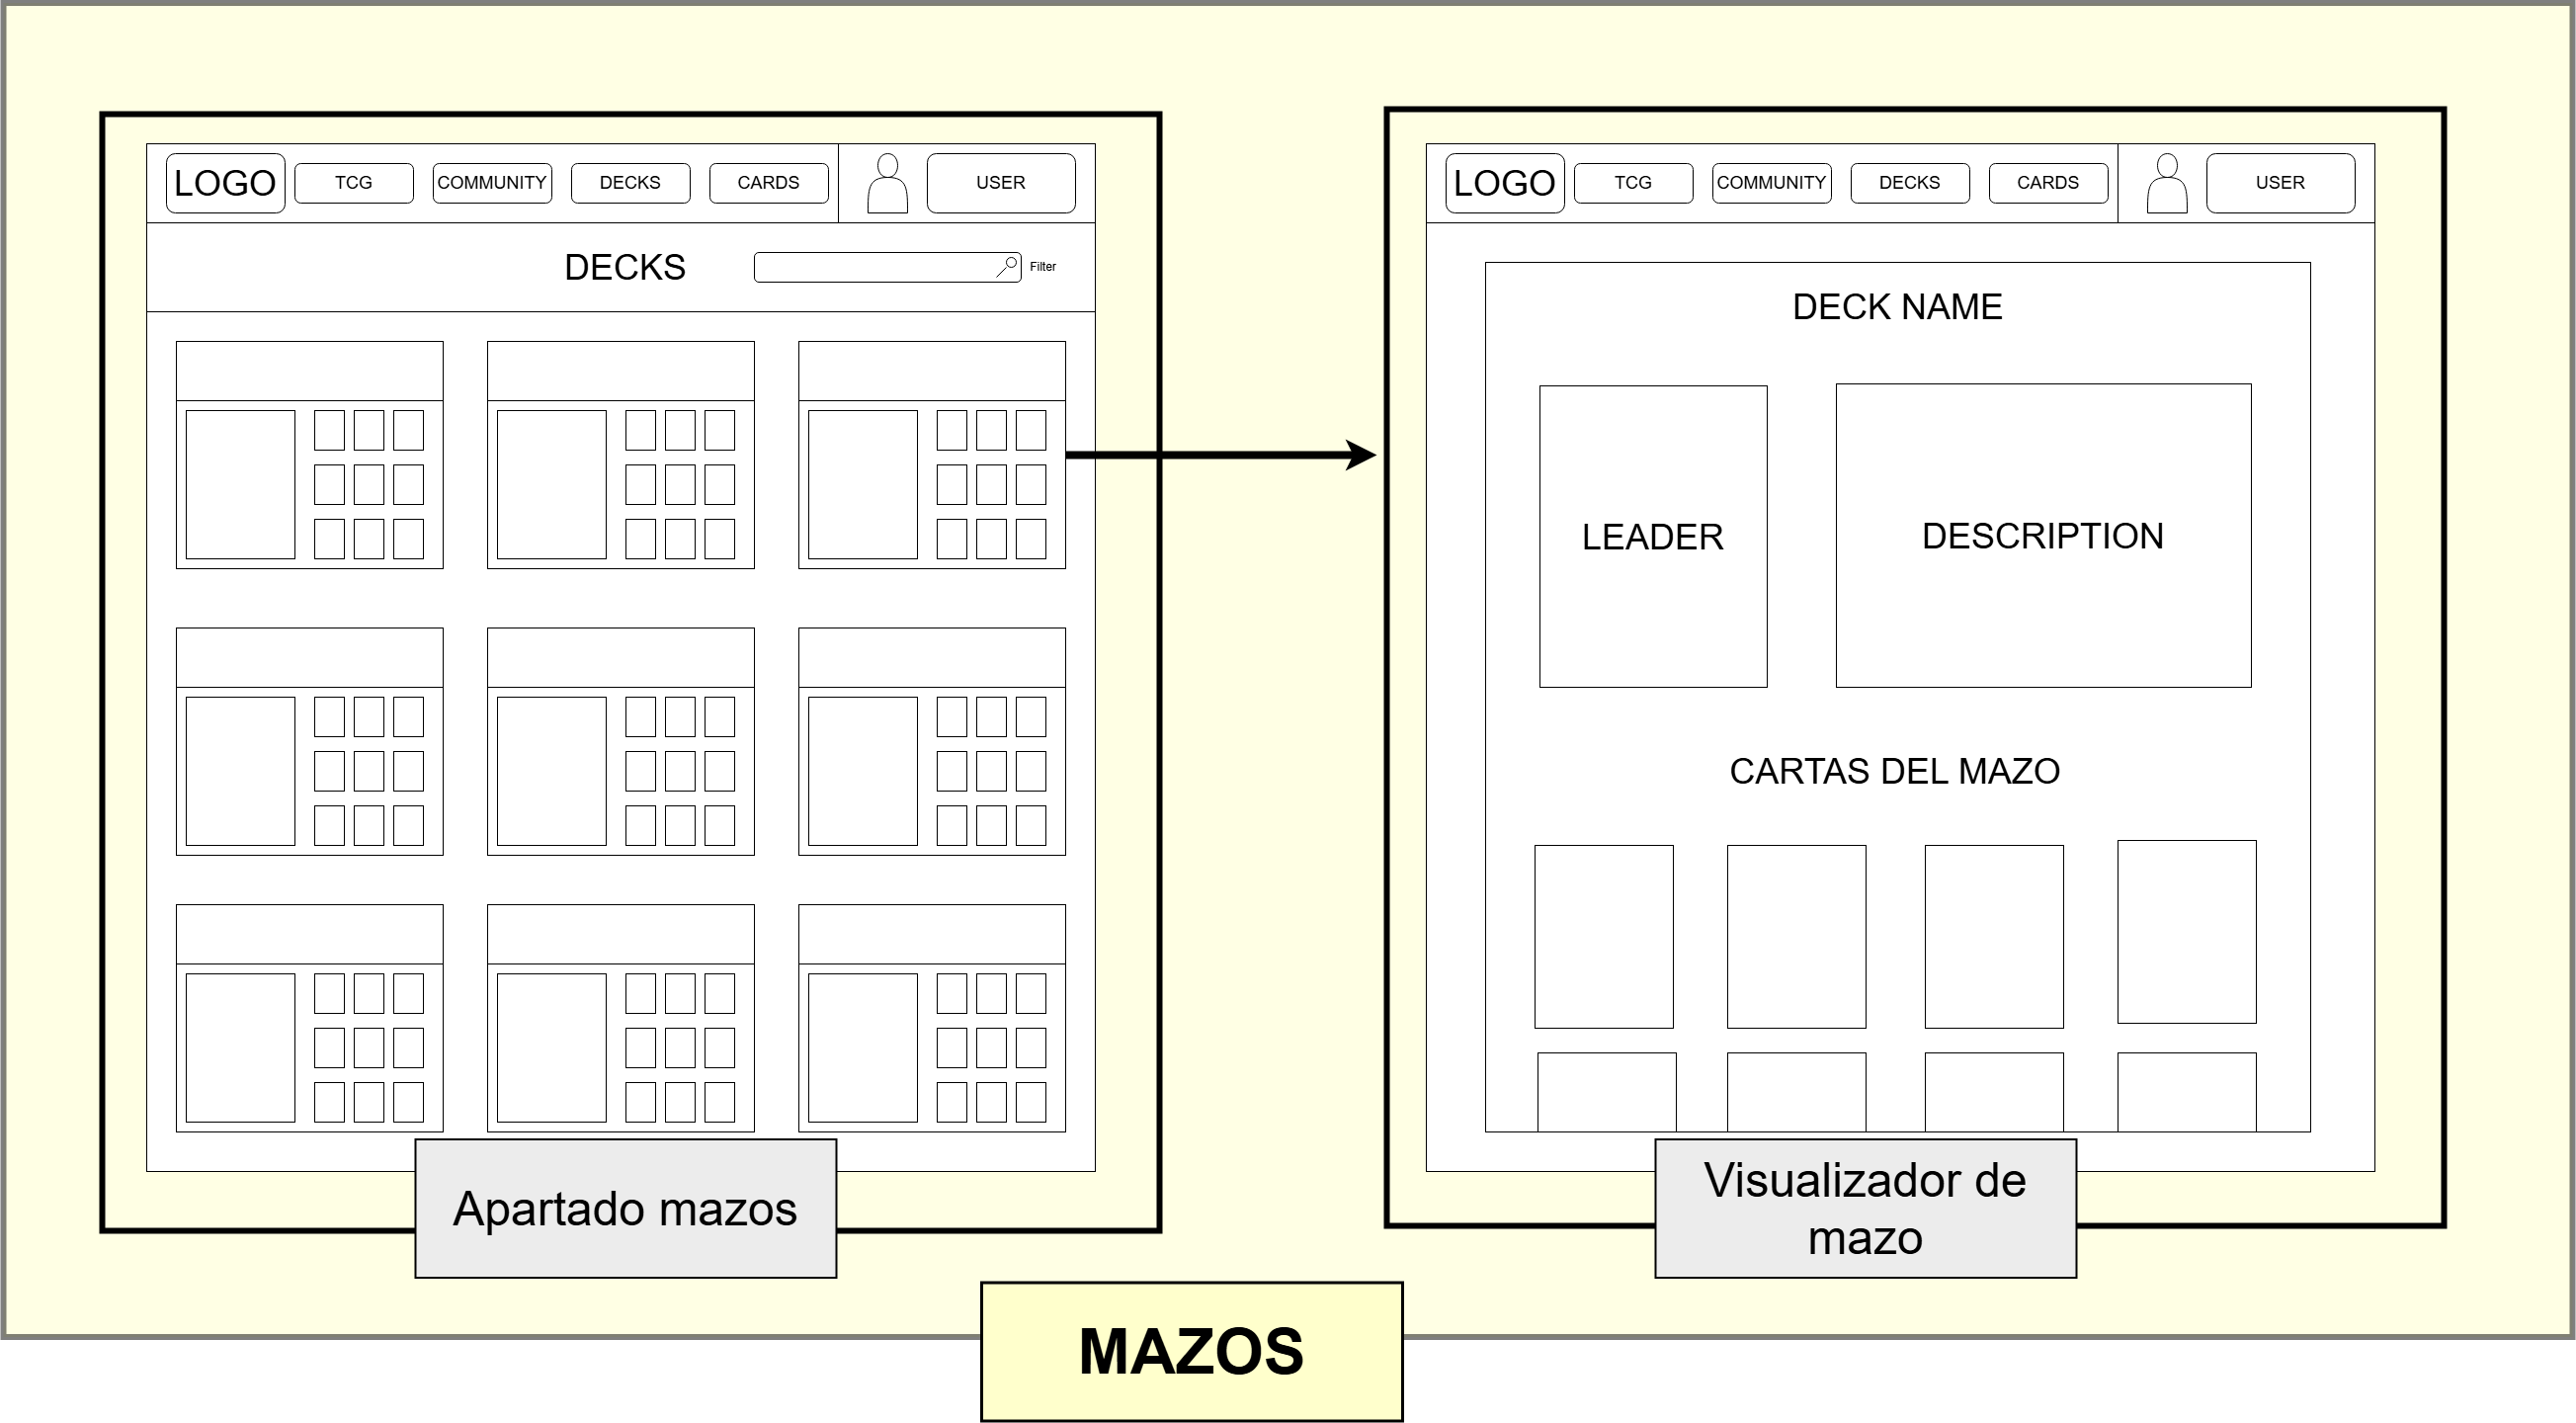
\includegraphics[width=0.85\textwidth]{Recursos/Boceto2_Mazos.png}
		\caption{\textbf{Boceto de la pestaña de mazos}}
	\end{figure}
	Esta pestaña incluye una lista con los elementos visuales de los diferentes mazos, tanto mazos \textit{META} introducidos por los administradores como los creados por la comunidad y los creados por el propio usuario, añadiendo también la opción de filtrar la búsqueda por elementos clave o buscar por nombre. Seleccionando un mazo concreto se nos abrirá el visualizador del mazo. Aquí podemos obtener información en detalle del mismo: el nombre del mazo, la carta \textit{Líder} del mazo, una descripción de este y la lista de cartas que lo compone.
	
	\begin{figure}[H]
		\centering
		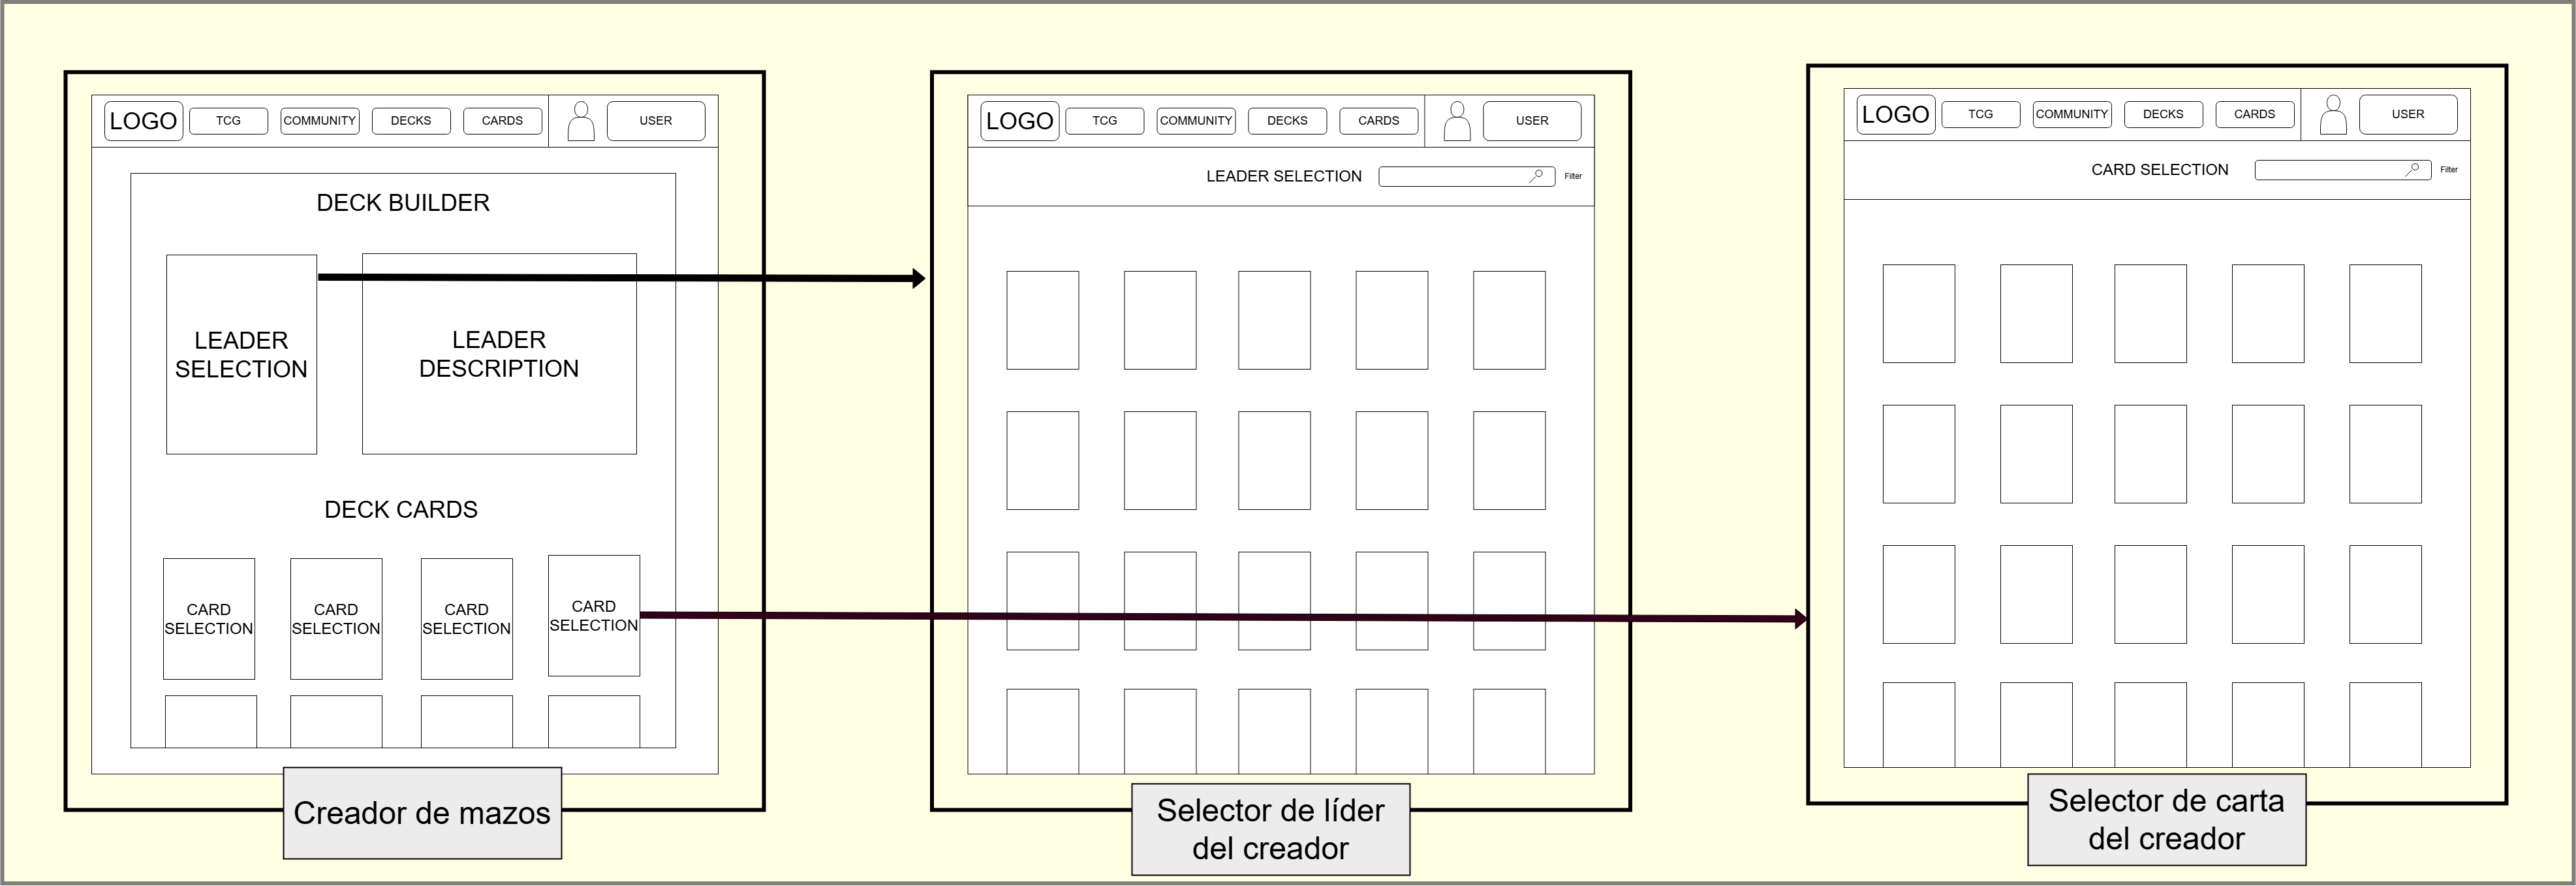
\includegraphics[width=0.85\textwidth]{Recursos/Boceto2_CreadorMazos.png}
		\caption{\textbf{Boceto de la pestaña del creador mazos}}
	\end{figure}
	Ahora observamos el apartado del creador de mazos. La vista es similar a la visualización de mazos de la comunidad, con la diferencia de que inicialmente no habrá cartas ni información de ningún tipo. \\
	
	Al seleccionar el apartado de la carta \textit{Líder} se nos abrirá un selector de cartas muy parecido a la lista entera de cartas (explicado en el siguiente apartado). Se pedirá al usuario que seleccione el color en el que esté basado el mazo que quiere crear (dentro del mundo del juego de One Piece hay cartas con diferentes colores, cada color tiene una mécanica diferente) y a raíz de eso saldrá la lista de líderes filtrada por el color seleccionado. \\
	
	De la misma forma se abrirá una lista de cartas normales al seleccionar el apartado de cartas normales, filtradas ya con el color del líder.
	
	\subsubsection{Cartas}
	
	\begin{figure}[H]
		\centering
		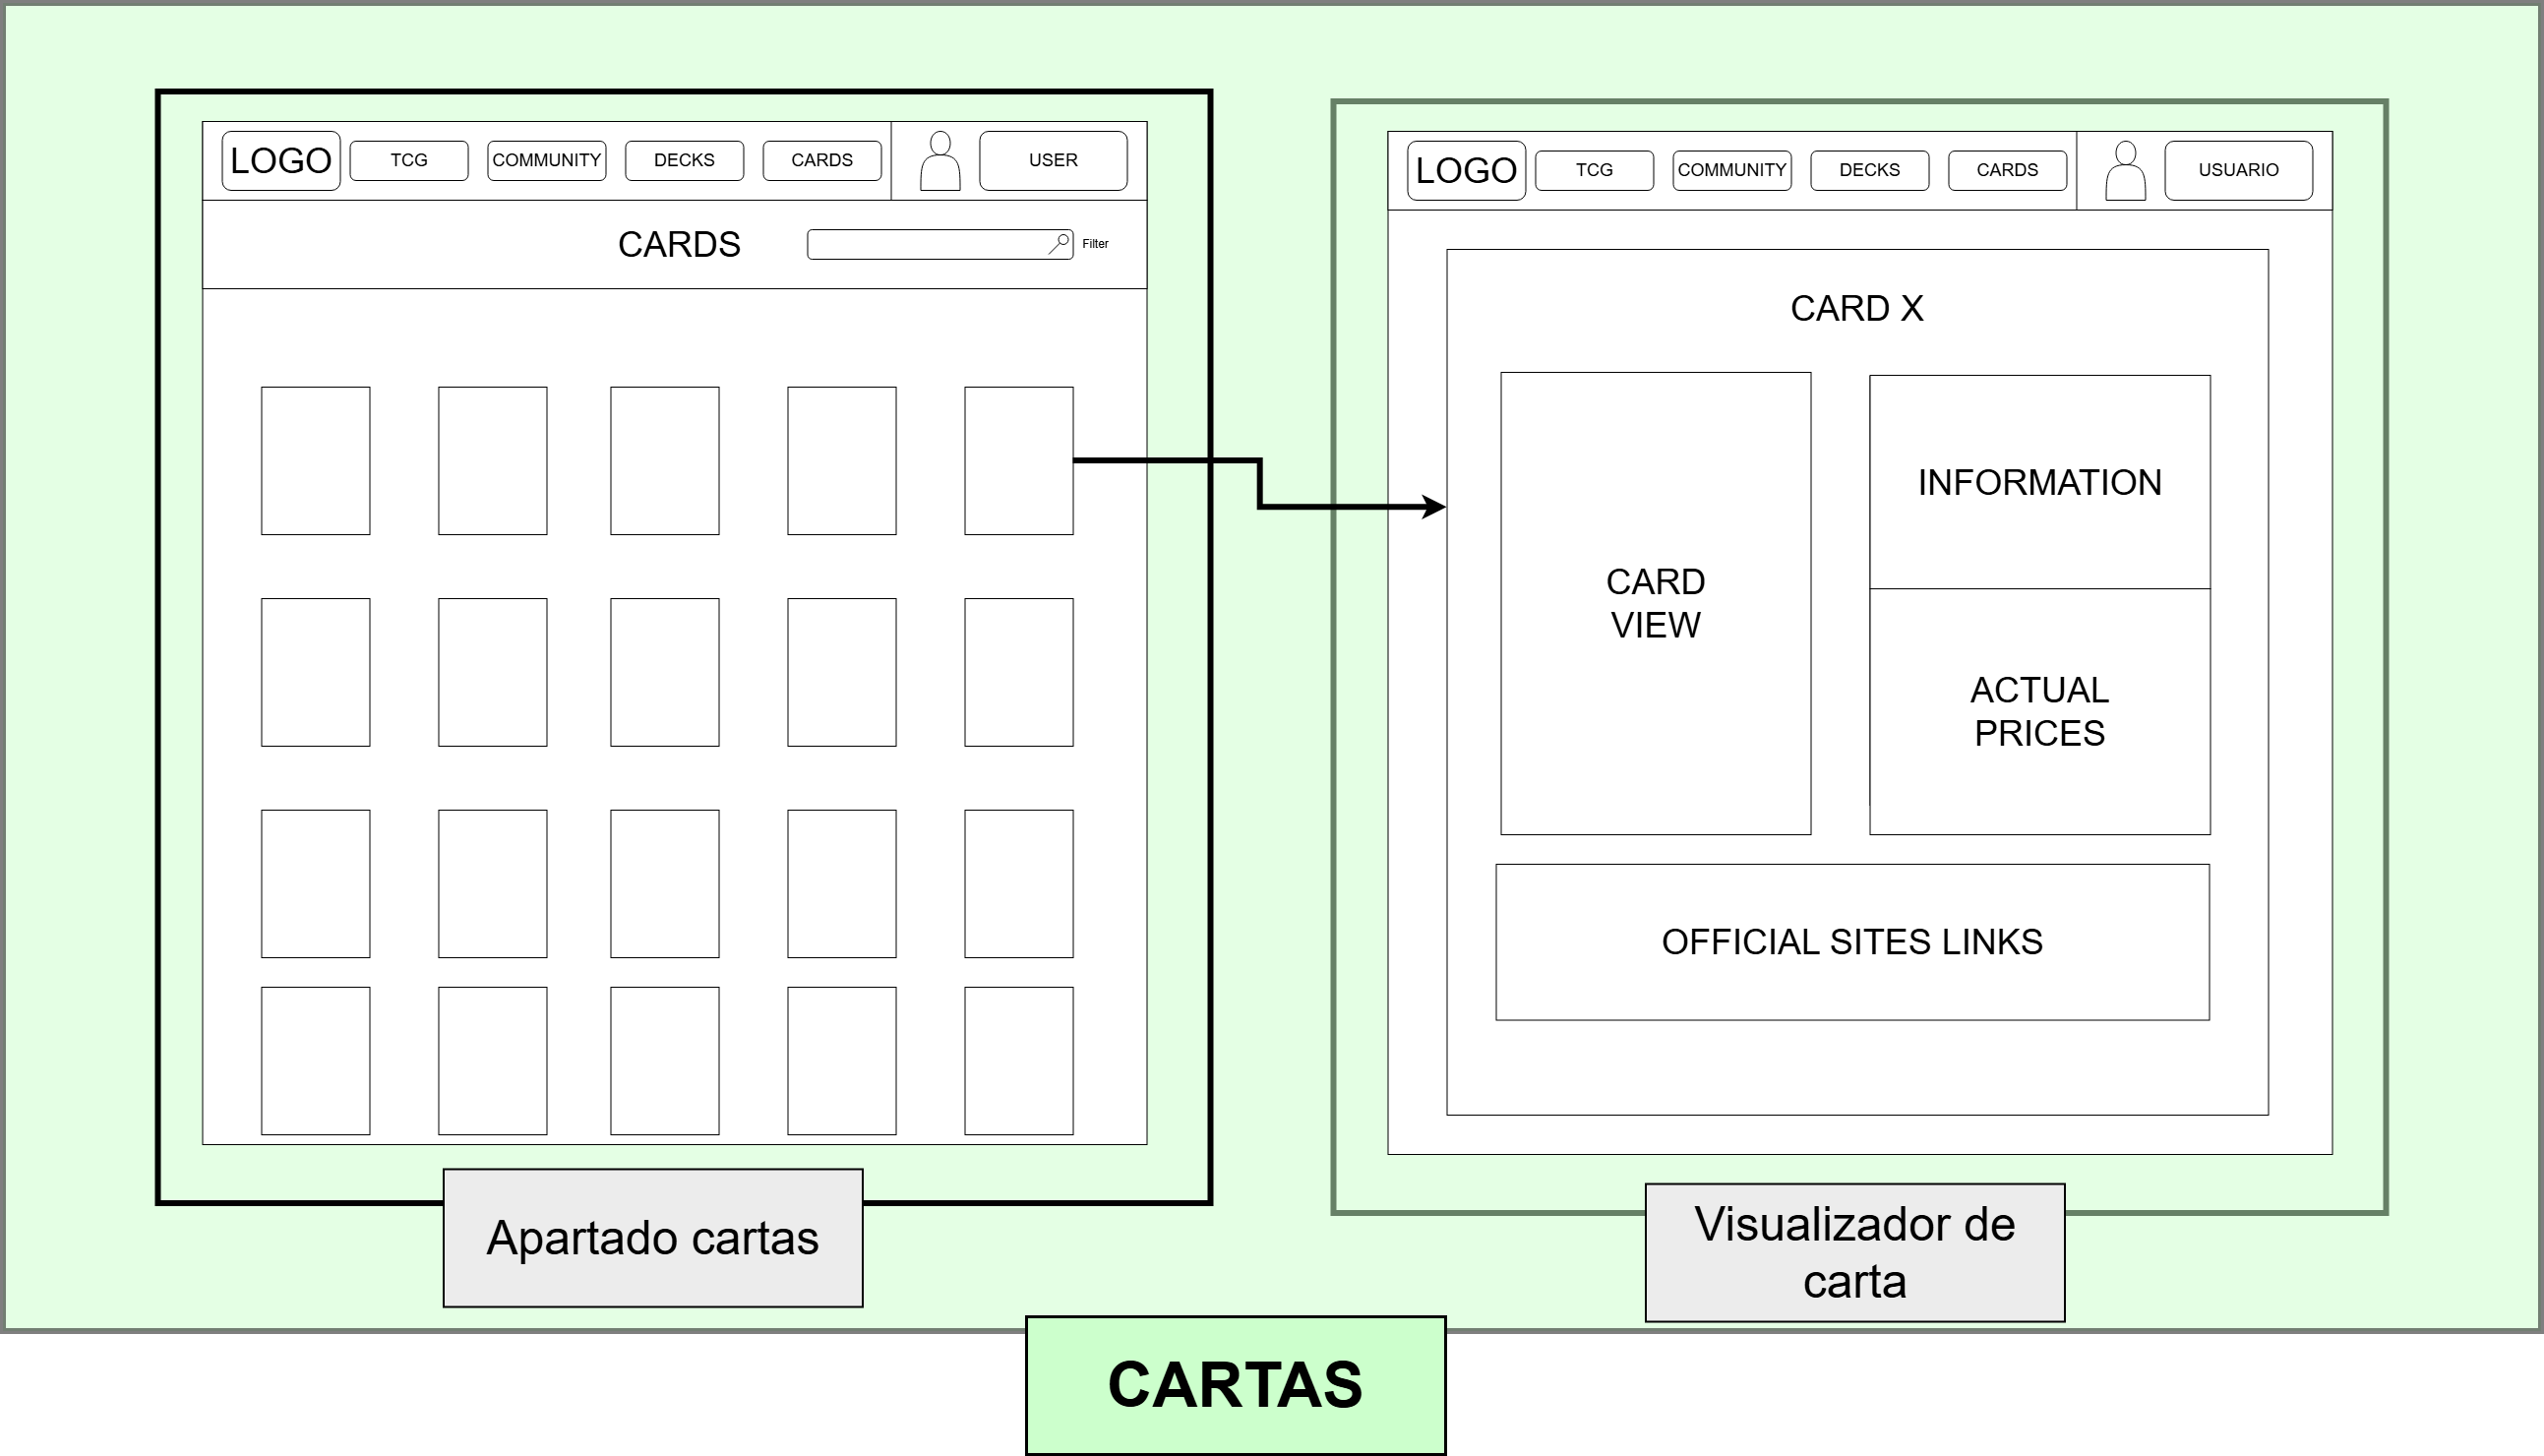
\includegraphics[width=0.85\textwidth]{Recursos/Boceto2_Cartas.png}
		\caption{\textbf{Boceto de la pestaña de cartas}}
	\end{figure}
	Similar a la pestaña de mazos, la vista de cartas nos incluye la lista de todas las cartas existentes. Encontramos diversos filtros de búsqueda (color, coste, daño, mecánica, etc.) que nos ayudan a encontrar las cartas que más convengan al usuario. Si se selecciona una carta podemos visualizar información en detalle: El nombre de la carta, una imagen de ella, el texto de información que está incluido en la carta, el precio en la web de compraventa y links a la página oficial del juego relacionados con ella.
	\newpage   
	\section{Implementación de funcionalidades.}
	En este punto del desarrollo pasamos de una web estática a una aplicación web basada en JSP, Servlets, DAOs, clases de dominio y una base de datos relacional en MariaDB. 
	A partir de este punto vamos a ir añadiendo y documentando la parte dinámica de nuestra web, es decir, la funcionalidad.
	\subsection{Mapa del sitio web}
	\begin{figure}[H]
		\centering
		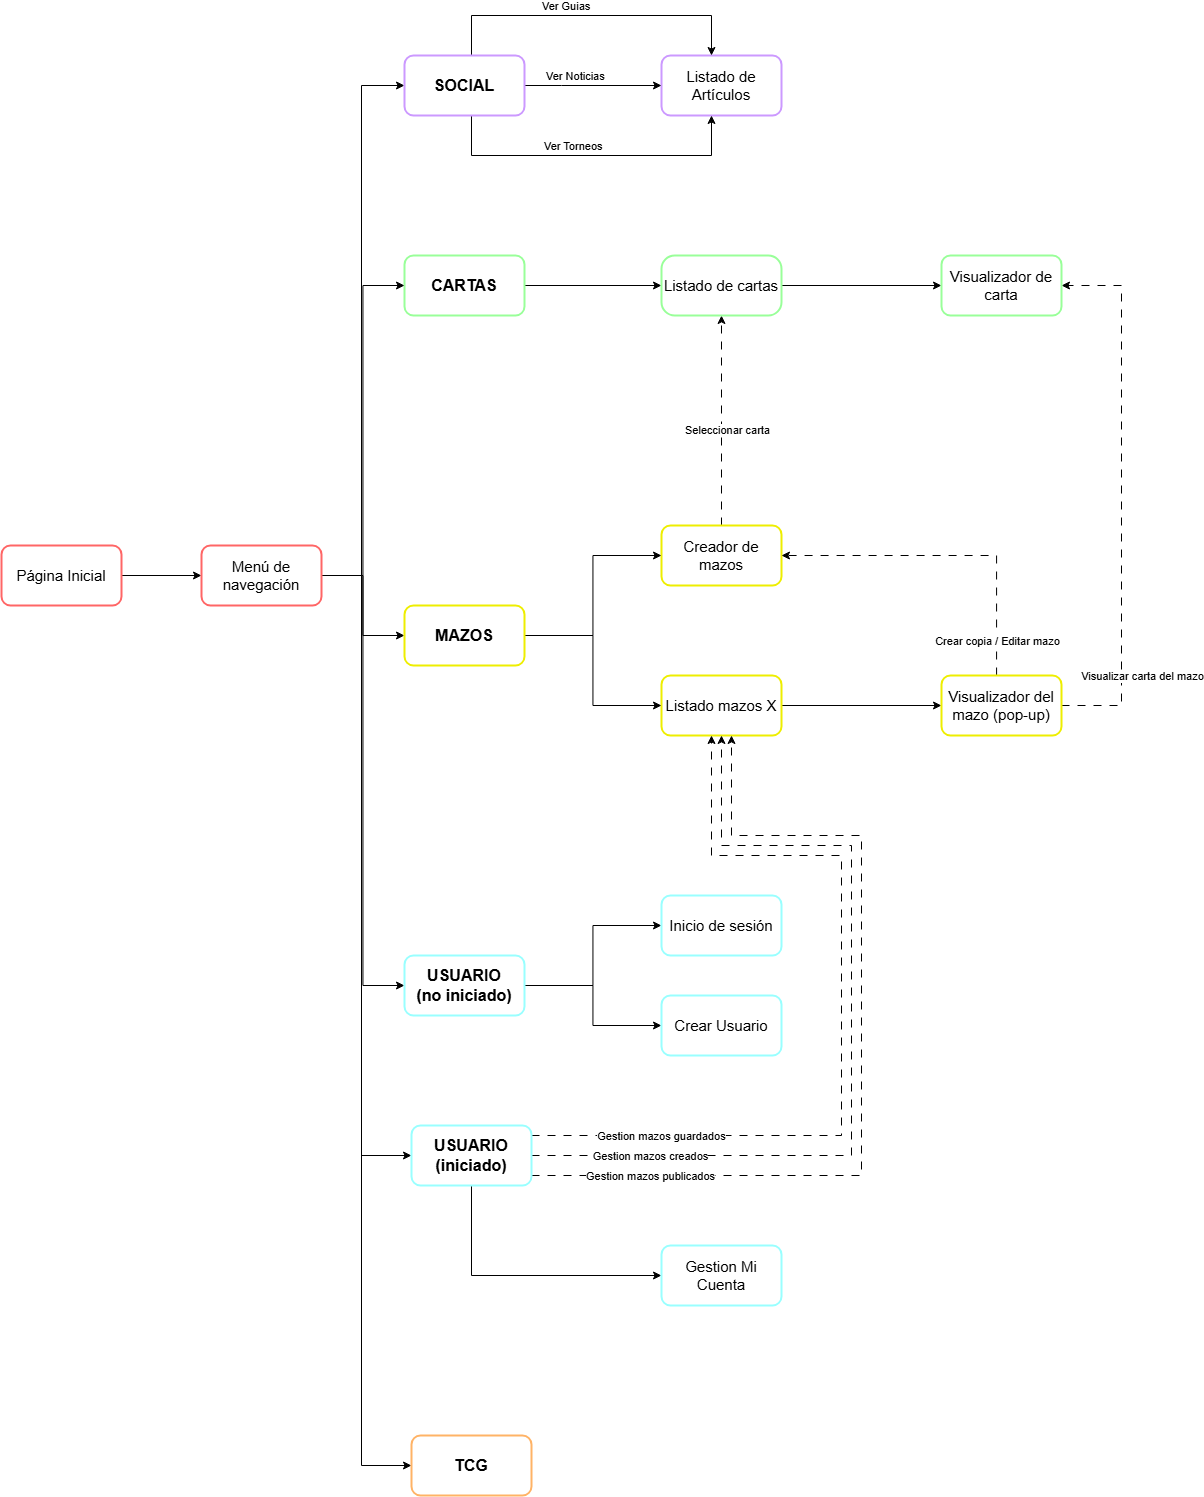
\includegraphics[width=0.7\textwidth]{Recursos/Mapa Card Partner v3.png}
		\caption{Estructura jerárquica y mapa del sitio web de Card Partner.}
		\label{fig:mapa_sitio}
	\end{figure}
	Nuestro diseño está centrado en la navegabilidad, permitiendo un acceso rápido a las diferentes funcionalidades del sitio web desde el \textit{header} de la web.\\
	
	\subsection{Estratificación por niveles del mapa de \textit{Card Partner}}
	Para facilitar la comprensión del mapa mostrado, vamos a añadir una explicación concisa sobre la arquitectura de la información que va a usar nuestra aplicación, dividida en niveles en función de los clicks o interacciones necesarias que tiene que realizar el usuario para llegar a dicha funcionalidad.\\
	Partiremos desde el \textbf{nivel 0} o \textbf{el punto de entrada}. Es aquél en el que se encuentra la \textbf{página principal}, el punto de acceso de todo usuario a nuestra aplicación y a su vez el menú que permitirá el acceso al resto de apartados.\\
	\subsubsection{Nivel 1: \textit{header} y navegabilidad}
	\textbf{El \textit{header}}: es el motor de navegabilidad principal de nuestra web. Se encuentra en la parte superior de cada una de las vistas y nos permite dividir la web en las 4 grandes secciones que constituyen el siguiente nivel, de esta manera el usuario final podrá navegar por las diferentes funcionalidades de la web de manera cómoda e intuitiva.\\
	
	Esto nos da acceso a todas las \textbf{herramientas y listados}:
	\begin{itemize}
		\item \textbf{SOCIAL:}  apartado donde el usuario final podrá encontrar noticias, artículos y guías sobre el juego. Se mostrarán 3 subsecciones como menús desplegables, los cuales permitirán acceder a cada una de estas vistas. Estas vistas ueden describirse como el \textbf{Listado de Artículos}, que mostrará contenidos de categorías de artículos diferentes (Noticias, Guías o Torneos) según a cual se acceda. Haciendo click en el artículo se redirigirá al usuario al sitio externo referido del artículo.
		\item \textbf{CARTAS:} esta opción da acceso al \textbf{listado de cartas} del TCG, donde el usuario podrá clickar sobre cada una de ellas para así poder acceder a una vista detallada de la seleccionada, dirigiendo al usuario al \textbf{Visualizador de carta}.
		\item \textbf{MAZOS:}  apartado a que agrupa todas las herramientas relacionadas a los mazos, permitiendo al usuario realizar acciones sobre este conjunto de cartas. 
		\item \textbf{USUARIO:} sección de la web donde el cliente podrá realizar una serie de accines en función de su estado.\\
		Si no ha iniciado sesión, aparecen las opciones correspondientes para que pueda autenticarse en el sistema, una vez hecho esto, se le devolverá al \textbf{nivel 0} con una modificación en el \textbf{nivel 1} donde  se mostrarán las secciones de \textbf{Gestión de Mi Cuenta} y las secciones de \textbf{Gestión de mazos creados}, \textbf{Gestión de mazos publicados} y \textbf{Gestión de mazos guardados}, que redirigirá al \textbf{Listado de Mazos} con los diferentes contenidos respectivamente, y a su vez podrá redirigir al \textbf{Creador de mazos} para editar los mazos del usuario.
		\begin{figure}[H]
			\centering
			\begin{subfigure}{0.45\textwidth}
				\centering
				
\includegraphics[width=\textwidth]{Recursos/HeaderConLogin.jpg}
				\caption{\textit{Header cuando el usuario tiene un \textit{login} válido}}
				\label{eqHCL}
			\end{subfigure}
			\hfill 
			\begin{subfigure}{0.45\textwidth}
				\centering
				
\includegraphics[width=\textwidth]{Recursos/HeaderSinLogin.png}
				\caption{Header cuando el usuario \underline{no} tiene un \textit{login} válido}
				\label{HSqeL}
			\end{subfigure}
		\end{figure}
		\item \textbf{TCG:} El apartado TCG mostrará la posible ampliación a futuro de la página web que cambiará el contexto del juego de cartas referido en toda la página.
		
	\end{itemize}
	
	\newpage
	\subsection{Nivel 2: visualizadores y flujos verticales}
	En él encontramos las acciones que requieren 2 click por parte del usuario, donde ya se llega a una funcionalidad en concreto de la página, vamos a describir cada uno de estos apartados:
	\begin{figure}[H]
		\centering
		\begin{subfigure}{0.45\textwidth}
			\centering
			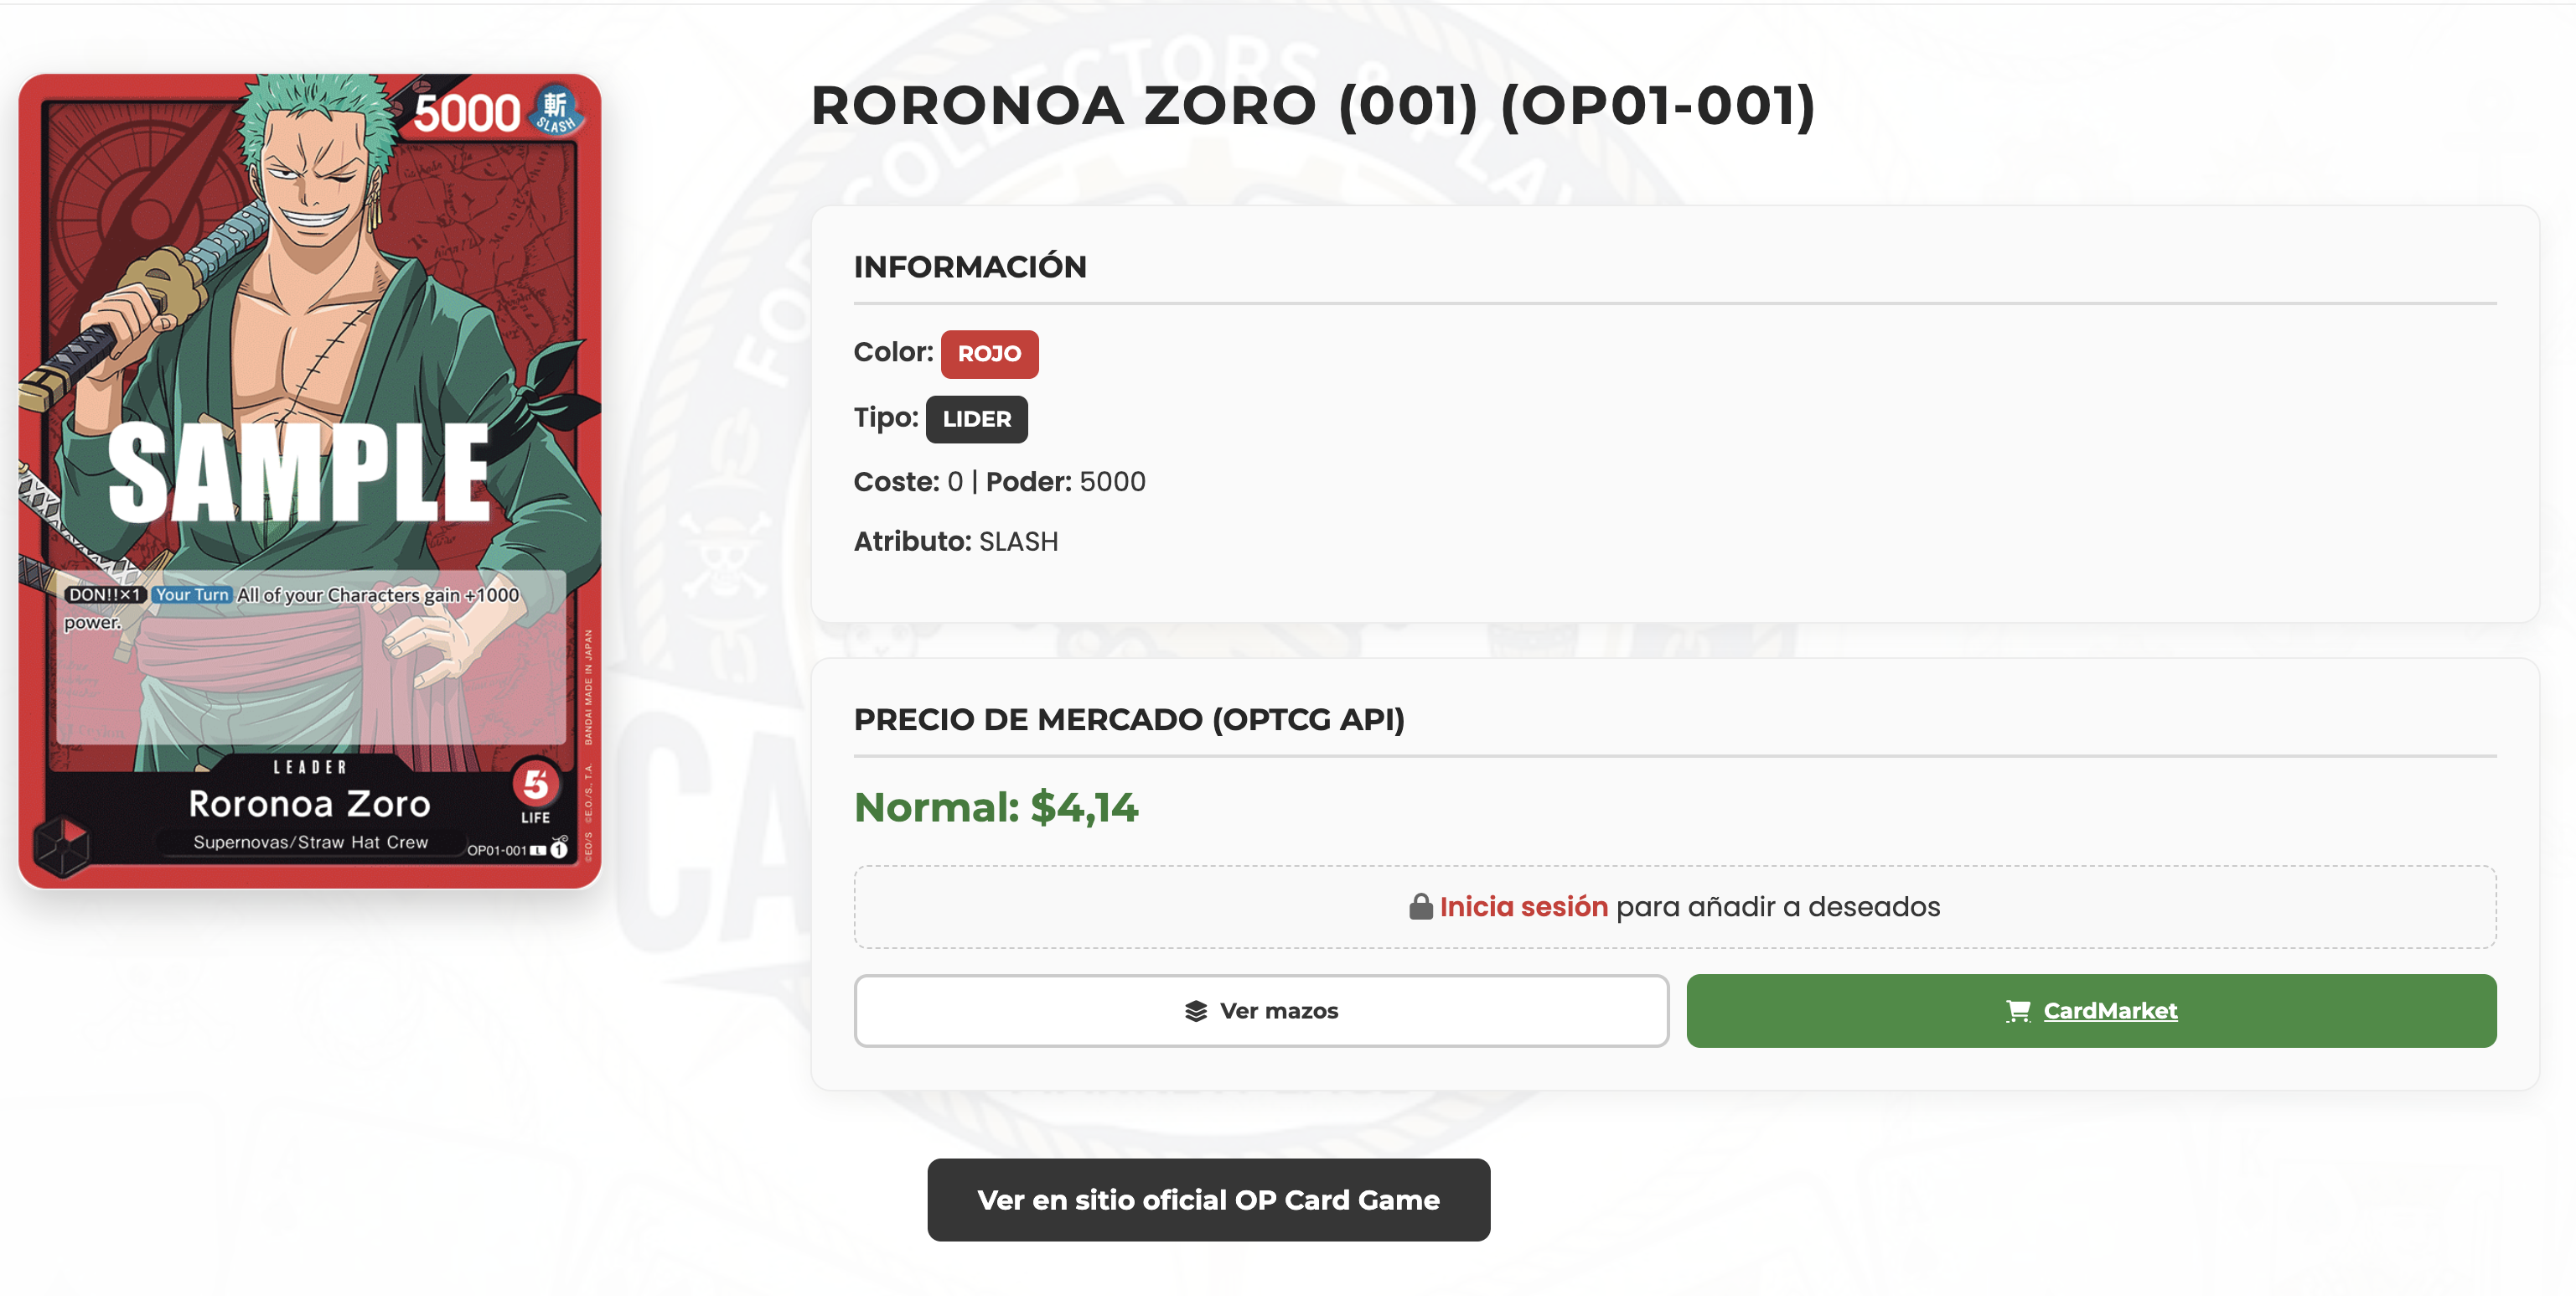
\includegraphics[width=\textwidth]{Recursos/visualizadorCarta.png}
			\caption{El \textbf{visualizador de carta} muestra los detalles concreto de una carta seleccionada por el usuario.}
			\label{VewqC}
		\end{subfigure}
		\hfill 
		\begin{subfigure}{0.45\textwidth}
			\centering
			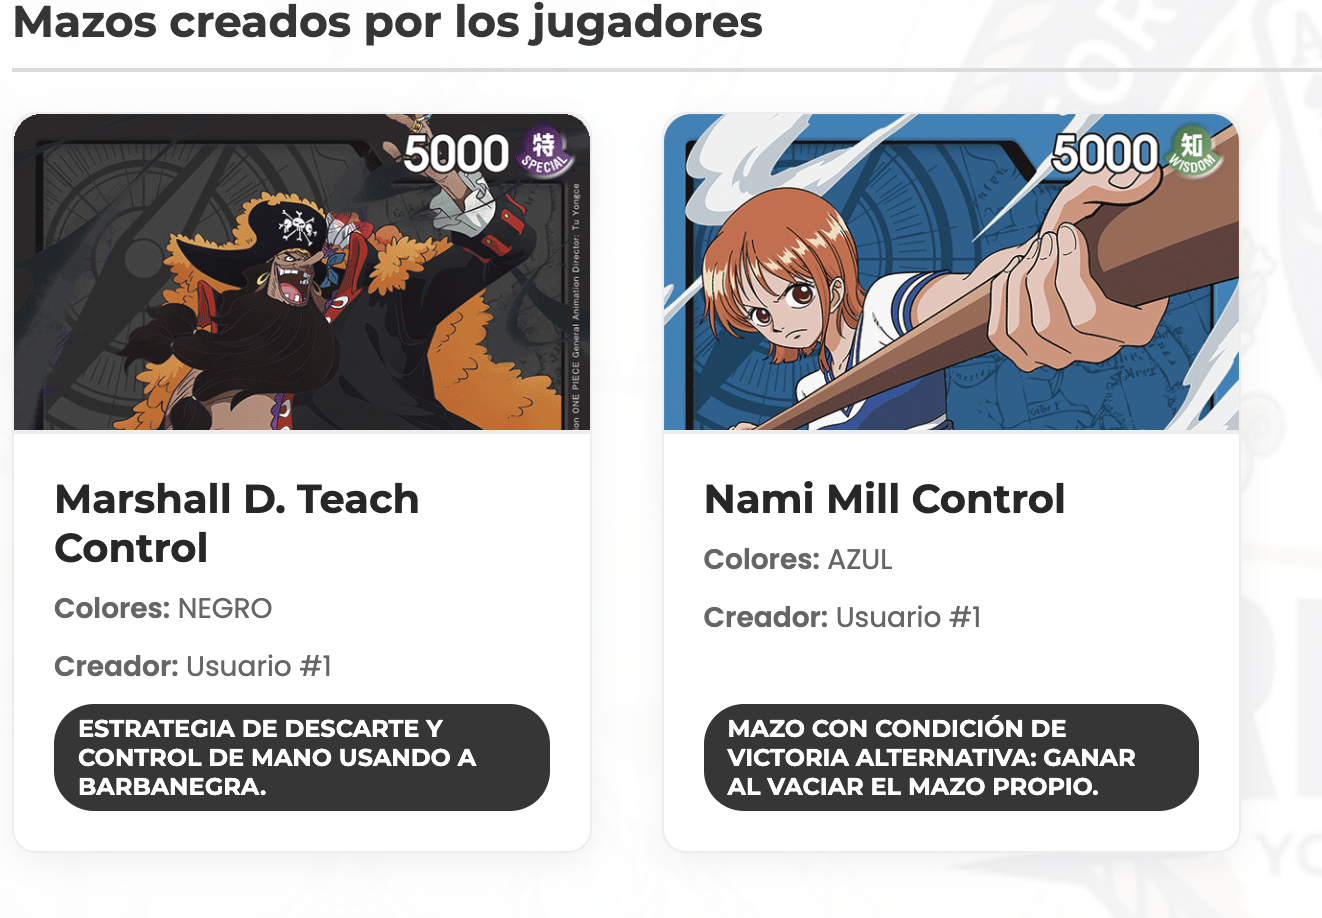
\includegraphics[width=\textwidth]{Recursos/Mazos.png}
			\caption{Misma estructura para los  \textit{comunity} y \textit{meta decks}, se muestra una lista de los mazos de cada sección con una pequeña descripción y la imagen del líder de cada uno de ellos}
			\label{VqeeM}
		\end{subfigure}
	\end{figure}
	\begin{figure}[H]
		\centering
		\begin{subfigure}{0.45\textwidth}
			\centering
			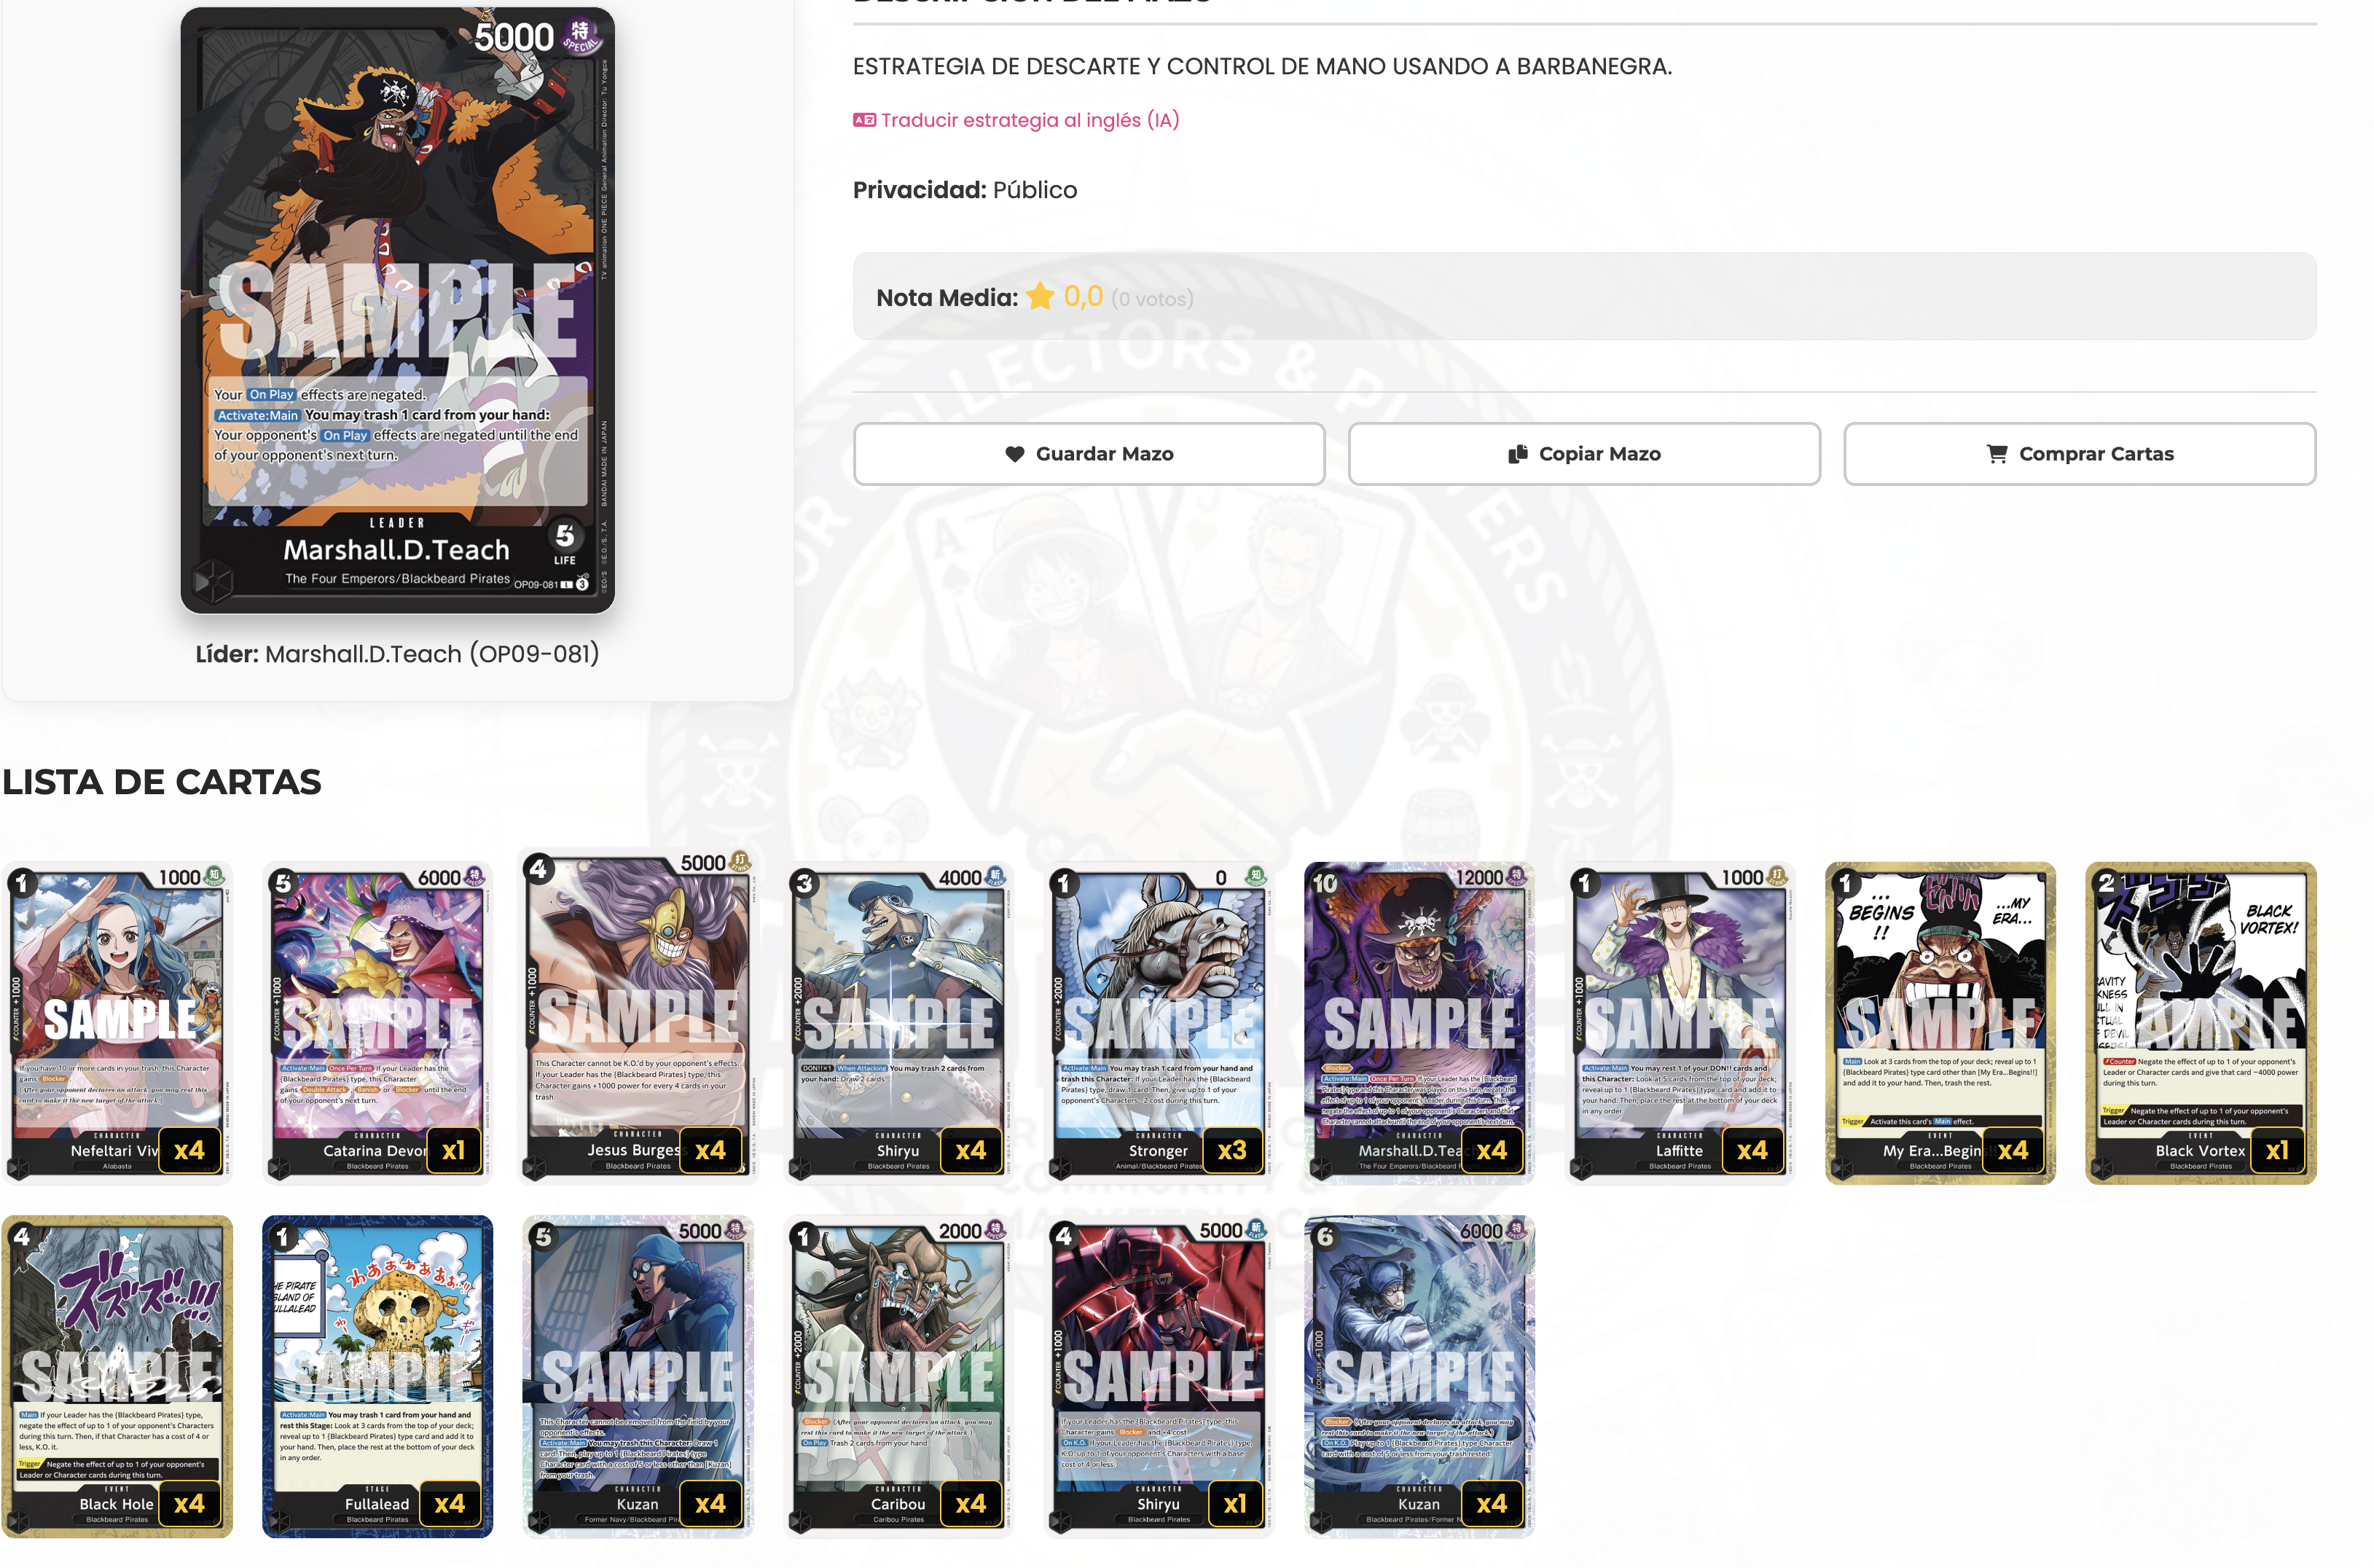
\includegraphics[width=\textwidth]{Recursos/Visualizador de Mazo.png}
			\caption{El usuario podrá consultar todas las cartas de un mazo, con las recomendaciones de cantidad de copias de cada una de ellas.}
			\label{VMazo}
		\end{subfigure}
		\hfill 
		\begin{subfigure}{0.45\textwidth}
			\centering
			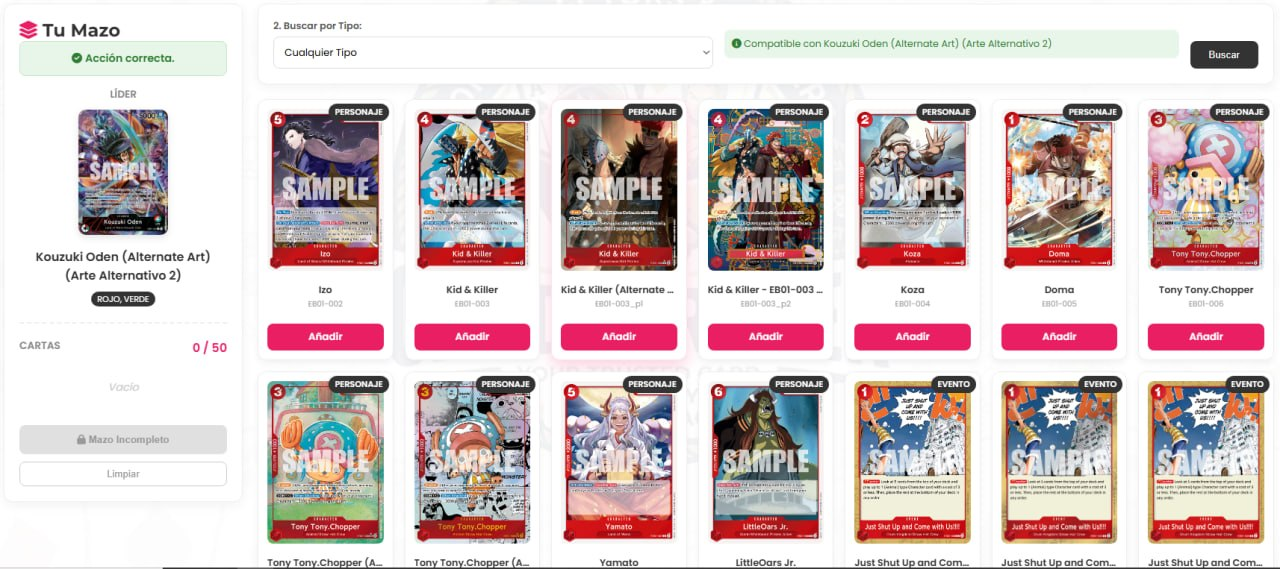
\includegraphics[width=\textwidth]{Recursos/CreadorMAzos.jpg}
			\caption{Vista para la creación de los mazos con un filtro por líder para que sólo se muestren las cartas compatibles con el arquetipo y color del mismo.}
			\label{VCeqeqqwM}
		\end{subfigure}
	\end{figure}
	\begin{figure}[H]
		\centering
		% Columna izquierda: Imagen (45% del ancho de página)
		\begin{minipage}{0.5\textwidth}
			\centering
			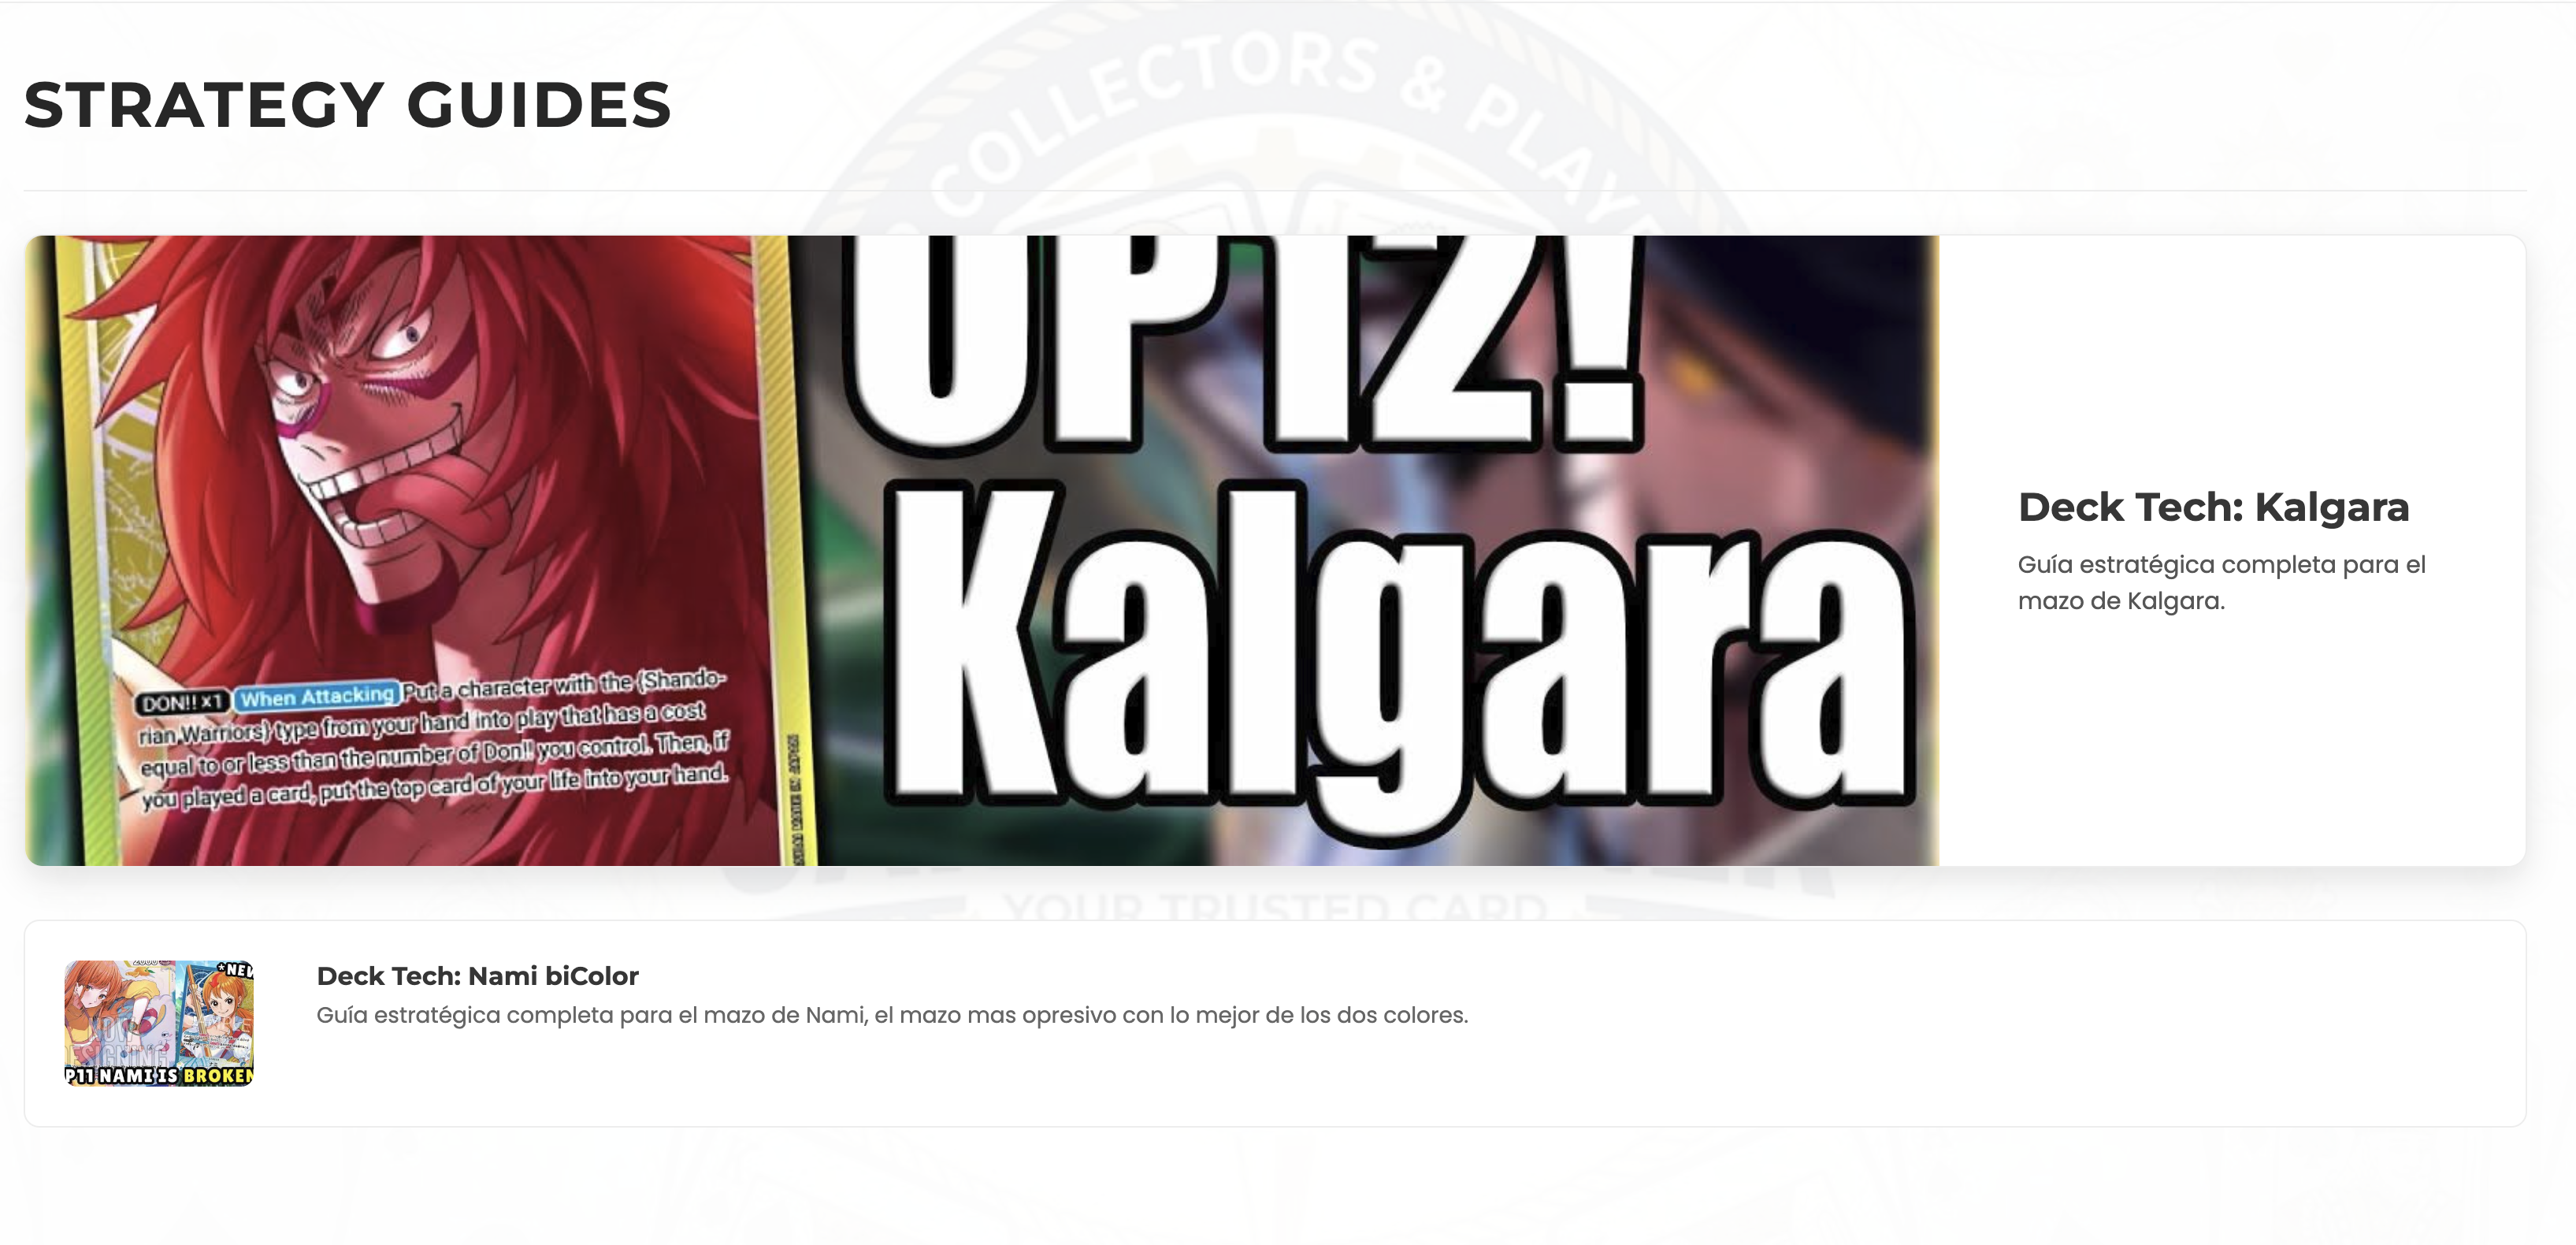
\includegraphics[width=0.85\textwidth]{Recursos/PanelGuias.png}
			\caption{Estructura social, tomando como ejemplo el apartado de Guías}
		\end{minipage}
		\hfill % Espacio elástico de separación entre las dos columnas
		% Columna derecha: Lista de atributos (50% del ancho de página)
		\begin{minipage}{0.45\textwidth}
			En el apartado de \textit{Social} de la web, tenemos 3 categorías, \textbf{guías}, \textbf{noticias} y \textbf{torneos}, las cuales siguen una estructura similar, una entrada principal con el contenido más representativo del momento, y una lista de entradas las cuales redirigen a sitios externos.\\
			Hemos tomado la decisión de descartar la redirección, puesto que consideramos que supone mucho trabajo para los administradores del sitio el tener que estar constantemente redactando artículos cuando ya hay medios dedicados a cubrir cada uno de estos campos. Sin embargo, lo que sí que harán los responsables, será un filtrado para tener sólo información relevante y actualizada, ya que estar informado de un TCG es parte fundamental del ciclo de vida del jugador.
		\end{minipage}
	\end{figure}
	\newpage
	
	\subsection{Flujos de navegación}
	Ya tenemos clara la estructura y aspecto visual de la página, así que ahora mostraremos unos casos de ejemplo de las acciones o menús necesarios para que un usuario pueda realizar las acciones principales definidas en el punto \ref{AccionesUsuario}
	\subsubsection{Consulta de mazos META}
	El usuario accede página Inicial, desde allí en el \textit{header} se encontrará con varios desplegables, entre ellos \textit{DECKS} que mostrará varias opciones, una de ellas será \textit{META decks}.
	\begin{center}
		\textbf{Página Inicial} $\rightarrow$ \textbf{DECKS} $\rightarrow$ \textit{\textbf{META decks}}
	\end{center}
	\subsubsection{Consultar noticias}
	El usuario, desde  el \textit{header}, accede al apartado SOCIAL, en el menú desplegable, seleccionará \textit{NEWS}.
	\begin{center}
		\textbf{Página Inicial} $\rightarrow$ \textbf{SOCIAL} $\rightarrow$ \textbf{Ver Noticias} $\rightarrow$ \textbf{NEWS}
	\end{center}
	
	\subsubsection{Consulta de cartas específica }
	Desde el \textit{header}, el usuario selecciona \textit{CARDS} Esto le lleva al catálogo general, donde tras aplicar filtros y buscar la carta deseada, hace clic sobre ella para abrir una vista detallada con toda su información.
	\begin{center}
		\textbf{Página Inicial} $\rightarrow$ \textbf{CARDS} $\rightarrow$ \textbf{Selección de carta} $\rightarrow$ \textbf{Visualizador de carta}
	\end{center}
	
	\subsubsection{Consultar los detalles de una carta incluida en un mazo}
	Mientras el usuario estudia la composición de una baraja, se encuentra con una carta que no conoce y necesita ver sus atributos, efectos o precio de mercado.\\
	Partimos desde el  visualizador del mazo, el usuario hace clic sobre una carta específica del listado, la web le redirigirá directamente la carta específica mediante el Visualizador de carta, sin tener que buscarla manualmente en el catálogo.
	\begin{center}
		\textbf{Página Inicial} $\rightarrow$ \textbf{\textit{DECKS}} $\rightarrow$ \textbf{Listado mazos X} $\rightarrow$ \textbf{Visualizador del mazo} $\rightarrow$ \textbf{Visualizador de carta}
	\end{center}
	
	\subsubsection{Consulta de una de las guías de juego}
	Desde el \textit{header} el usaario se dirige a la sección \textit{SOCIAL}, dentro del menú despegable, selecciona \textit{GUIDES}, tras lo cual, el sistema mostrará el Listado de guías filtrando la base de datos para enseñar únicamente el contenido de aprendizaje, permitiendo al usuario acceder a las explicaciones.
	\begin{center}
		\textbf{Página Inicial} $\rightarrow$ \textbf{SOCIAL} $\rightarrow$ \textbf{GUIDES} $\rightarrow$ \textbf{Listado de guías}
	\end{center}
	
	% Apartado MAPA WEB:\\
	
	% El mapa no incluye explícitamente una página de perfil propio (gestión de datos del usuario, cambio de contraseña) como nodo diferenciado; aparece como "Gestión Mi Cuenta" pero sin desarrollar qué contiene.\\
	
	% La sección TCG aparece en el mapa como una opción de ampliación futura, pero ya está implementada en las páginas estáticas. Podría haberse integrado mejor en el mapa como sección funcional actual.\\
	
	
	\subsection{Base de datos}
	Para esta parte del desarrollo empezamos a implementar una bbdd, en concreto nos decantamos por  MariaDB a través de XAMPP para facilitar el trabajo de gestión y diseño, ya que permite usar phpMyAdmin desde navegadores web y gestionar la base de datos de manera visual y exportar o importar los scripts de creación e inserción de datos,  además de otras herramientas útiles (como el meter archivos .csv).
	
	\subsection{Cambios del Modelo de Dominio a Entidad-Relación}
	Para traducir el modelo de dominio realizado en la práctica 2 al \textbf{modelo entidad-relación} se han efectuado los siguientes cambios:
	\begin{itemize}
		\item \textbf{Usuario}: Se ha traducido la relación de \textit{Usuario} como clase padre de \textit{Jugador} y \textit{Admin} a una sola tabla \texttt{Usuario} y un atributo ROL que especifique qué tipo de usuario es.
		\item \textbf{Mazo}: Al igual que con \textit{Usuario}, la clase \textit{Mazo} se ha traducido a una única tabla \texttt{Mazo} y un atributo ES\_OFICIAL para hacer la distinción.
		\item \textbf{Relaciones *:*}: Las relaciones muchos a muchos entre \textit{Jugador}-\textbf{GUARDA}-\textit{Mazo}, \textit{Mazo}-\textbf{CONTIENE}-\textit{Carta} y \textit{Jugador}-\textbf{VALORA}-\textit{Mazo} se han traducido como las clases intermedias \texttt{GUARDA\_MAZO}, \texttt{CONTIENE\_CARTA} y \texttt{VALORACION} respectivamente.
		
	\end{itemize}
	
	\begin{figure}[H]
		\centering
		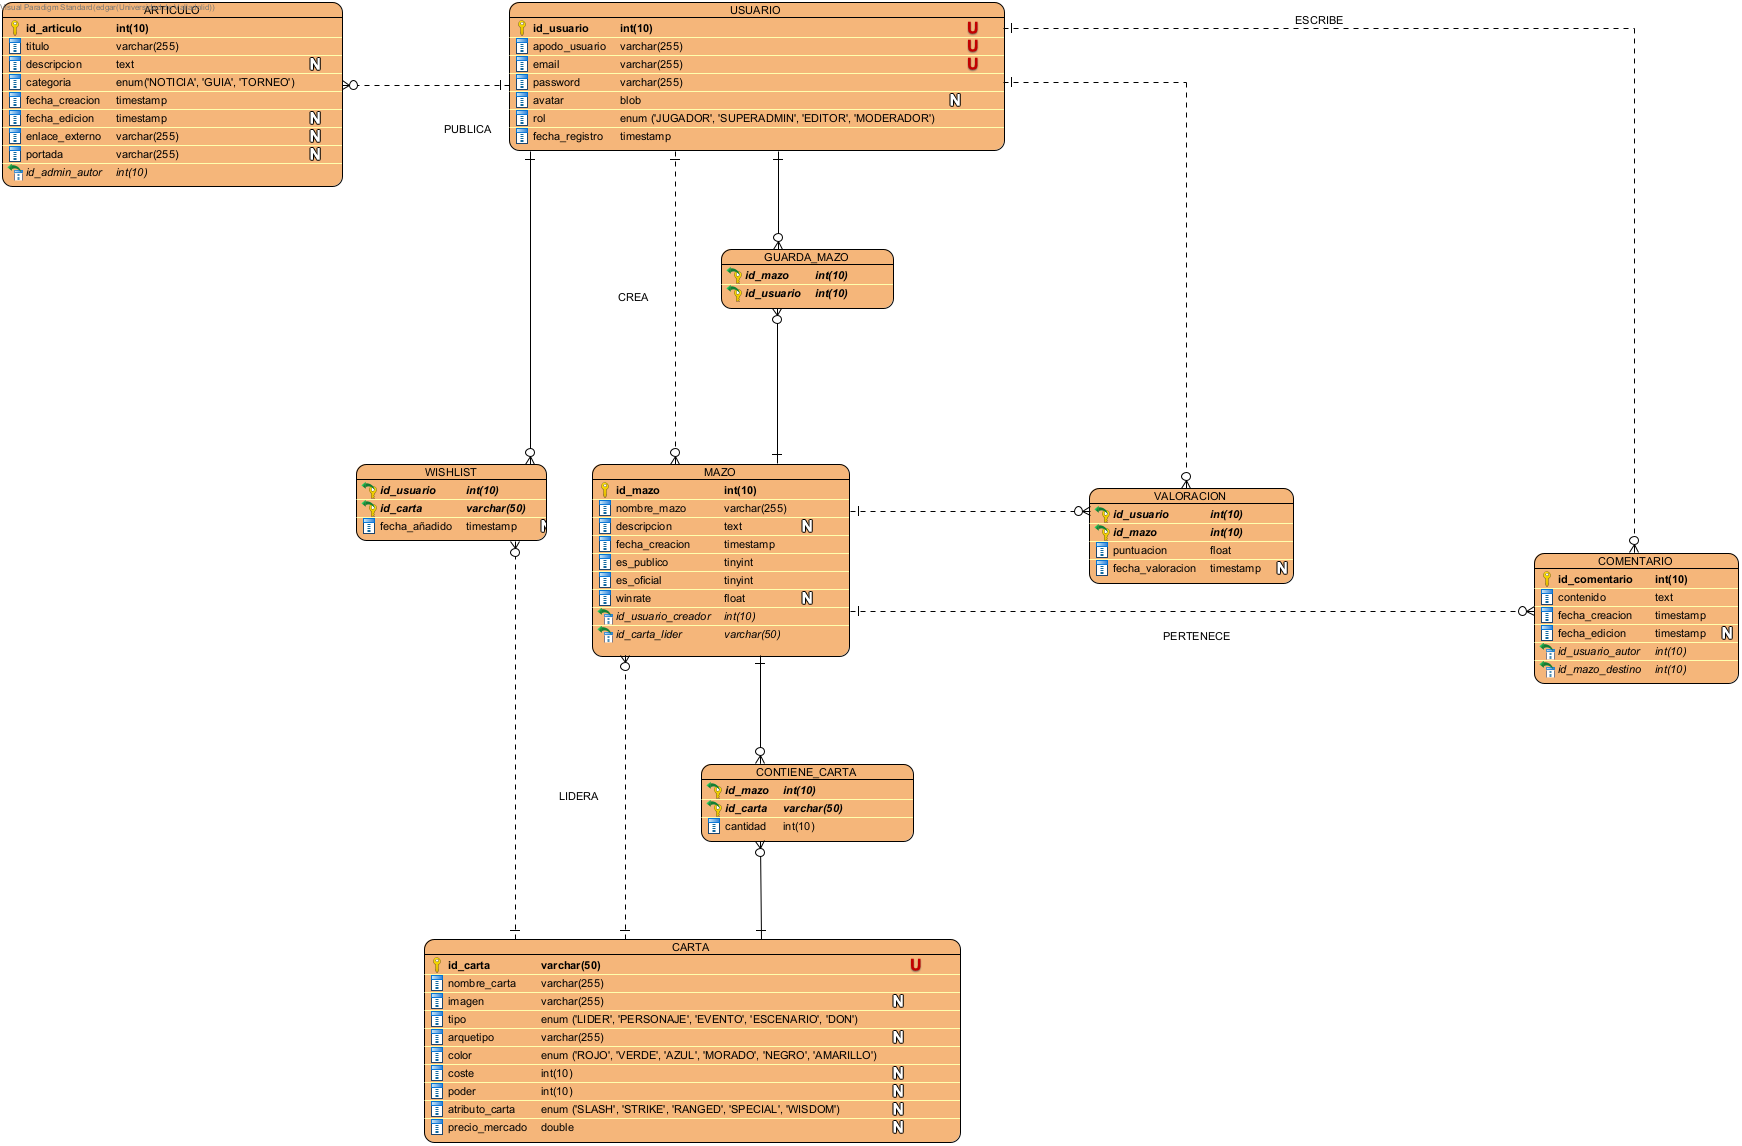
\includegraphics[width=1\textwidth]{Recursos/CardPartner_DBv2.png}
		\caption{Entidad-Relacion de la base de datos}
		\label{bbdeqedEsquema}
	\end{figure}
	
	
	\subsection{Estructura de la Base de Datos}
	
	Nuestra base de datos (\texttt{cardpartner\_db} ) está diseñada bajo un modelo relacional orientado a la gestión de una comunidad de juegos de cartas coleccionables (TCG). Su arquitectura se divide en cuatro pilares fundamentales:
	
	\subsubsection{Componentes Principales}
	
	\begin{itemize}
		\item \textbf{Gestión de Usuarios y Roles:} la entidad \texttt{USUARIO} centraliza el acceso y la seguridad. Empleamos un sistema de roles (\textit{Jugador, Editor, Moderador, Superadmin}), el cual es una traducción directa de los niveles de privilegios en el sistema.
		\item \textbf{Catálogo de Cartas y Mazos:} 
		\begin{itemize}
			\item \texttt{CARTA}: actúa como el diccionario técnico del juego, almacenando atributos estáticos como coste, poder, color y tipo.
			\item \texttt{MAZO}: representa la agrupación lógica de cartas creada por un usuario, vinculada obligatoriamente a una carta líder.
		\end{itemize}
		\item \textbf{Módulo de Comunidad:} la interacción social se articula a través de las tablas \texttt{VALORACION}, \texttt{COMENTARIO} y \texttt{GUARDA\_MAZO}, permitiendo la retroalimentación y la creación de bibliotecas personales.
		\item \textbf{Sistema de Contenidos:} la entidad \texttt{ARTICULO} permite a los administradores gestionar noticias, guías y torneos, manteniendo la plataforma actualizada.
	\end{itemize}
	
	\subsection{Resumen de Relaciones y Cardinalidad}
	Teniendo en claro la estructura de nuestra bbdd, pasaremos a explicar las relaciones entre entidades y las cardinales de las mismas.
	\begin{table}[H]
		\centering
		\begin{tabularx}{\textwidth}{l l X}
			\toprule
			\textbf{Relación} & \textbf{Tipo} & \textbf{Descripción} \\
			\midrule
			Usuario $\rightarrow$ Mazo & 1:N & Un usuario es autor de múltiples mazos. \\
			Mazo $\leftrightarrow$ Carta & N:M & Relación gestionada por \texttt{CONTIENE\_CARTA} con cantidades. \\
			Usuario $\leftrightarrow$ Mazo & N:M & Biblioteca personal y favoritos (\texttt{GUARDA\_MAZO}). \\
			Usuario $\rightarrow$ Articulo & 1:N & Relación de autoría para perfiles administrativos. \\
			\bottomrule
		\end{tabularx}
		\caption{Resumen de la Arquitectura de Datos} 
	\end{table}
	
	\subsection{APIs empleadas en nuestro sistema}
		Uno de los aspectos que teníamos en mente para aplicar respecto a entregas anteriores era el uso de APIs (\textit{Application Programming Interface}), la cual nos otorga la posibilidad de comunicarnos con otra aplicación de una manera sencilla, permitiéndonos introducir funcionalidades extra a \textit{Card Partner} sin tener que desarrollarlas nosotros mismos, consiguiendo así ahorrarnos tiempo y generar menos archivos.
	
	\subsubsection{API encargada de la obtención de cartas}
		Este era uno de los puntos pendientes de la anterior entrega, ya que como se ha podido ver en la figura \ref{fig:insertarCartas} teníamos una muestra limitada de cartas.\\
		Teniendo más tiempo, hemos implementado un código (se puede ver en la sección \ref{JAVAAPI} de los anexos) el cuál se encarga de hacer el papel de motor de sincronización de la plataforma, encargándose de generar el catálogo completo de cartas desde una \textit{API REST} externa (empleamos la librería Google \textbf{GSON}).\\
		
		El funcionamiento es simple, el sistema establece una conexión HTTP, descarga el archivo JSON correspondiente y lo procesa de manera iterativa, estableciendo unos \textit{timeouts} y métodos de \textit{parseo}, evitando fallos críticos del sistema al procesar nodos JSON nulos, variables faltantes o formatos numéricos inconsistentes, asegurando que solo se persista información limpia y válida. También traduce datos al castellano y nos permite añadir cartas que tienen más de un color.\\
		
		Una de las partes más tediosas de la práctica son los alter o artes alternativos, cartas que comparten el mismo id y los mismos atributos, variando únicamente el arte que muestran. Como no se pueden almacenar cartas con un mismo ID en la base de datos Nuestro código altera dinámicamente el identificador (añadiendo sufijos indexados) y el título de la carta, evitando así colisiones de claves primarias.
	\subsubsection{API de traducción}
		La clase \textit{GeminiAPI} (la cuál se puede consultar en la sección \ref{JAVAGEMINI} de los anexos) actúa como un servicio de traducción inteligente, integrándose mediante peticiones HTTP con la API de Groq y el modelo Llama-3, mandando prompts a la LLM y obteniendo las respuestas de manera casi inmediata. Hacemos especial hincapié en la robustez de las respuestas, para que no aparezcan caracteres raro (como puede ser la traducción de una ñ o una tilde si el texto está en inglés) empleando JSONs para la comunicación con el servicio e implementando un mecanismo para que, si la \textit{IA} no responde, se muestre el texto original en vez de un mensaje de error.\\
		
		Este módulo adapta dinámicamente sus prompts en función del contexto del texto original, permitiéndonos entrenar este modelo para que utilice jerga específica de TCG (como \textit{Ramp} o \textit{Rested}), o que mantenga un tono natural en los comentarios de los usuarios. 
	
	\subsection{Descripción de la funcionalidad implementada y justificación de la elección}
	
	
	\subsubsection{Gestión de usuarios y perfil}
	Desarrollamos un sistema de usuarios capaz de distinguir entre visitantes, jugadores registrados y administradores.\\
	 Los visitantes pueden consultar contenido público, como la lista de cartas, noticias, guías, torneos y mazos públicos mientras que los jugadores registrados disponen de acceso completo a todo el contenido público con el añadido de un perfil personalizado donde podrán gestionar sus datos, cambiar la contraseña, crear y guardar mazos, comentar y valorar los mazos de la comunidad. \\
	 Por último, los administradores tienen privilegios para publicar mazos oficiales y artículos, así como mantener el contenido de la web actualizado.\\
	
	Hemos decidido centralizar toda la gestión de datos en la sección de \textbf{Perfil}, permitiendo a los usuarios acceder a sus activos y configuraciones desde un único punto. Esta elección garantiza que la administración de la información sea intuitiva y accesible, evitando dispersión en múltiples páginas.
	
	\subsubsection{Catálogo de cartas y filtros}
	Para manejar el amplio repertorio de cartas que tiene el TCG de \textit{One Piece} hemos desarrollado filtros avanzados por nombre, color, tipo, coste y rareza, basándonos en la necesidad de los jugadores de localizar rápidamente cartas específicas y planificar la construcción de sus mazos de forma eficiente.\\
	A mayores la carta nos muestra el precio de mercado por el cual se vende en las plataformas online.
	
	\subsubsection{Gestión y creación de mazos}
	El constructor de mazos o \textit{Deckbuilder} ha sido implementado con ventanas emergentes modales que permiten filtrar y asignar la carta líder y así poder configurar la composición completa de un mazo, donde se aplica un filtro automático para mostrar sólo aquellas cartas compatibles por color y/o arquetipo con el líder.\\
	
	En este campo tenemos dos tipos de mazos, los oficiales o \textit{META} y los comunitarios, diferenciados a través de atributos como \texttt{es\_publico} o \texttt{winrate} para diferencialos. Esto permite que los jugadores puedan crear, guardar y consultar mazos de manera flexible, mientras que los mazos oficiales permanecen verificados y orientados a la escena competitiva.\\
	
	Además, se han creado vistas de detalle de mazo que muestran el precio total, estadísticas y cartas contenidas, facilitando la toma de decisiones al jugador y mejorando la experiencia de navegación.
	
	
	\subsubsection{Comunidad e interacción}
	Se ha integrado un sistema de comentarios y valoraciones en cada mazo, permitiendo que los usuarios registrados pueden publicar sus opiniones, sugerir cambios y puntuar mazos creados por otros usuarios.
	
	\subsubsection{Social}
	Como hemos mencionado en puntos anteriores, la sección de noticias, guías y torneos será gestionada por los administradores permitiéndonos mantener una calidad en los contenidos que se muestren en nuestra web consolidando a \textbf{Card Partner} como un punto de referencia dentro de la comunidad \textit{TCG.}
	
	\subsubsection{Sección TCG}
		Al inicio de este documento comentábamos que íbamos a emplear el juego de cartas de \textit{One Piece} como referencia, pero consideramos que si la fórmula funcionaba, adentrarnos en el resto de \textit{TCGs} sería una tarea sencilla, ya que simplemente habría que adaptar lo que ya tenemos a cada una de las mecánicas, por eso hemos dejado esta sección donde el usuario podrá encontrarse con los principales juegos del mercado.
		\begin{figure}[H]
			\centering	
			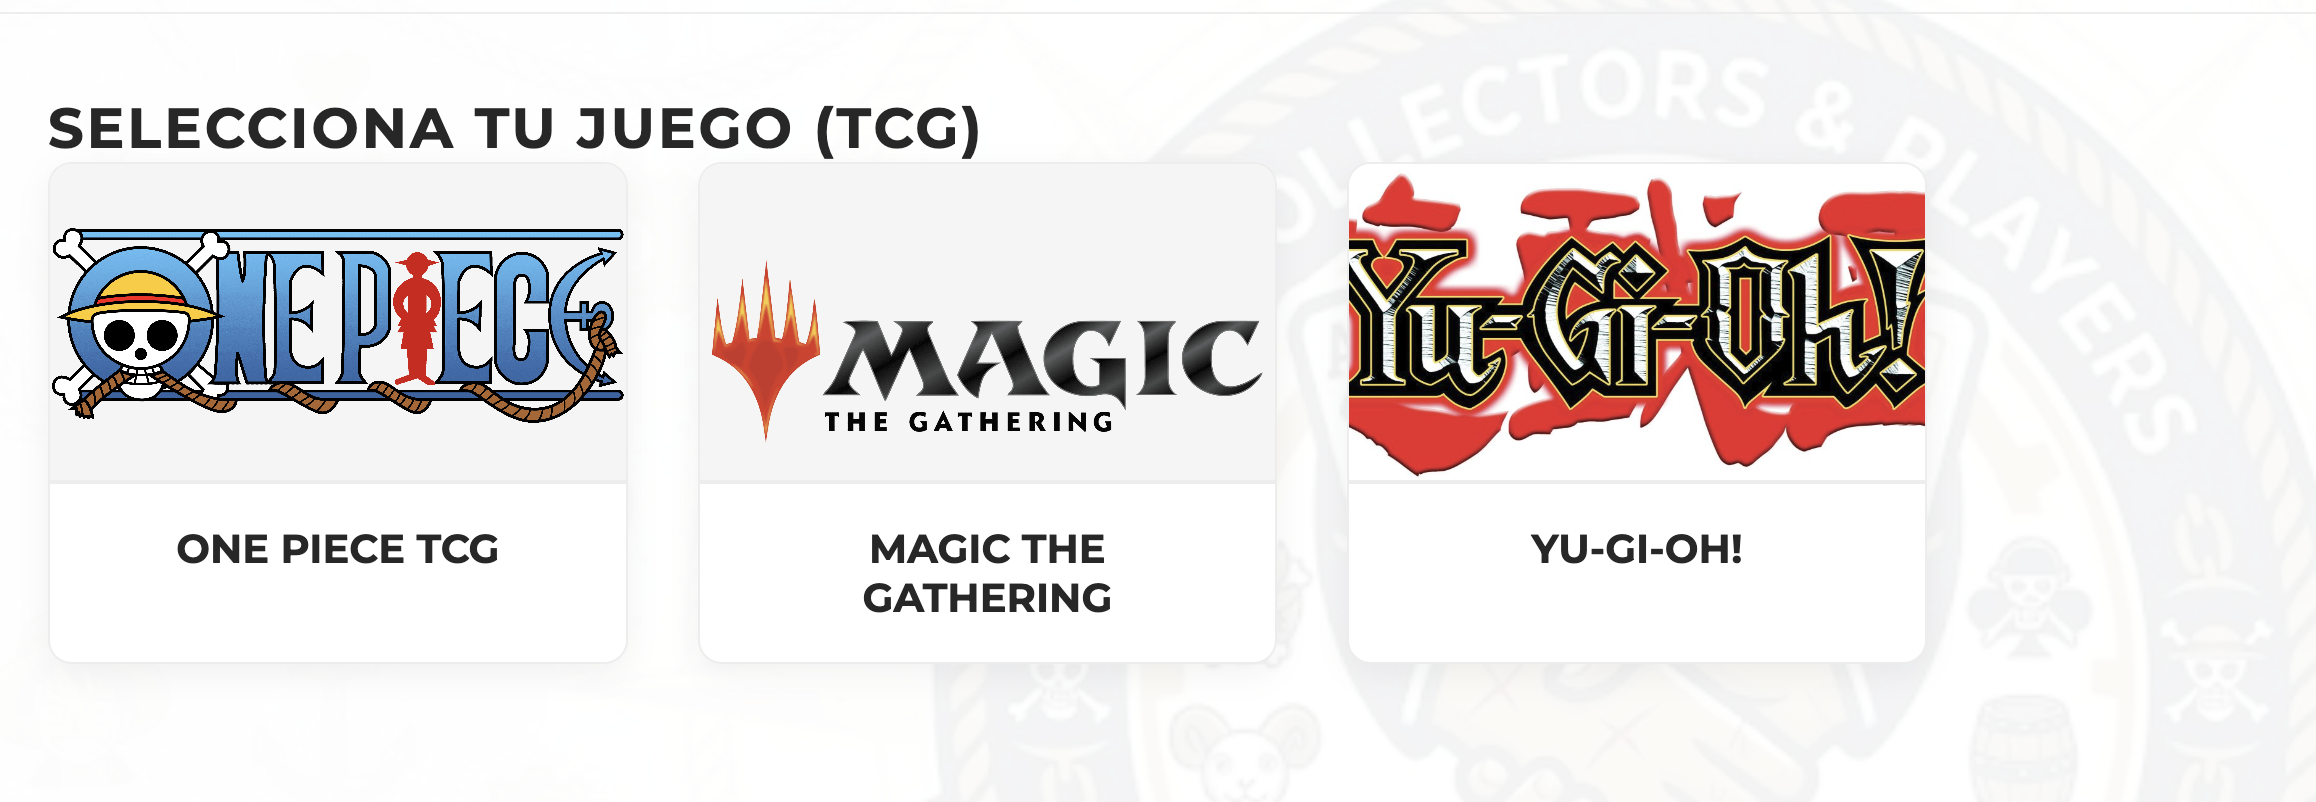
\includegraphics[width=\textwidth]{Recursos/TCG.png}
			\caption{\textit{Hub}de selección entre los TCGs}
		\end{figure}
	
	\subsection{Justificación de la elección}
	Hemos optado por implementar estas funcionalidades priorizando:
	
	\begin{itemize}
		\item Centralización de información y herramientas, evitando que los jugadores tengan que usar múltiples webs externas.
		\item Claridad y facilidad de uso, con un panel de perfil único y vistas modales en el constructor de mazos.
		\item Escalabilidad, permitiendo agregar nuevas cartas, mazos o secciones sin necesidad de reescribir la estructura base del sistema.
		\item Interacción social, fomentando la participación de la comunidad mediante comentarios y valoraciones.
		\item Coherencia con el modelo de dominio y la base de datos, asegurando que la estructura de información sea consistente y fácil de mantener.
	\end{itemize}
	
	Con estas decisiones, \textbf{Card Partner} ofrece una plataforma funcional, intuitiva y completa, que cubre las necesidades más importantes de los jugadores de TCG y justifica las elecciones de diseño realizadas en el desarrollo del sistema.
	
	\subsection{Instrucciones de ejecución del código}
	\begin{itemize}
		\item Ejecutar el script de \textit{setup\_db} (que se encuentran en \textit{CardPartner/sql/} o en el directorio raiz de SSW si se mira desde el repositorio de GitHub)
		\item Realizar la conexión con la bbdd en el Apache NetBeans
	\end{itemize}
	\begin{figure}[H]
		\centering
		% Primera imagen
		\begin{subfigure}[b]{0.3\textwidth}
			\centering
			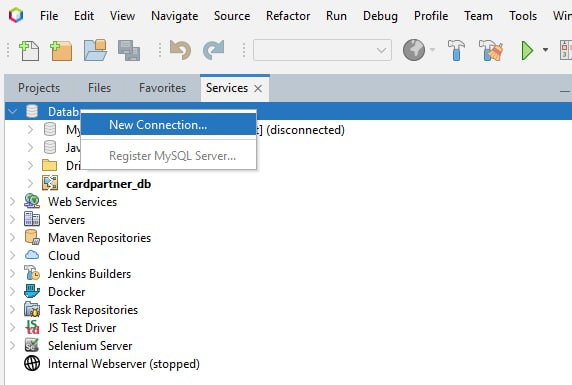
\includegraphics[width=\textwidth]{Recursos/Services.jpg}
			\caption{Vamos al menú de \textit{services} del editor}
		\end{subfigure}
		\hfill % Espaciado horizontal elástico
		% Segunda imagen
		\begin{subfigure}[b]{0.3\textwidth}
			\centering
			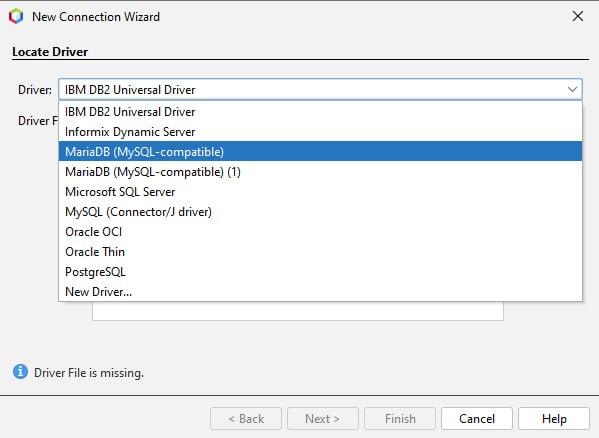
\includegraphics[width=\textwidth]{Recursos/DriverMDB.jpg}
			\caption{En el menú desplegable seleccionamos nuestra base de datos y buscamos el driver que se encuentra en la carpeta lib de nuestro proyecto}
		\end{subfigure}
		\hfill % Espaciado horizontal elástico
		% Tercera imagen
		\begin{subfigure}[b]{0.3\textwidth}
			\centering
			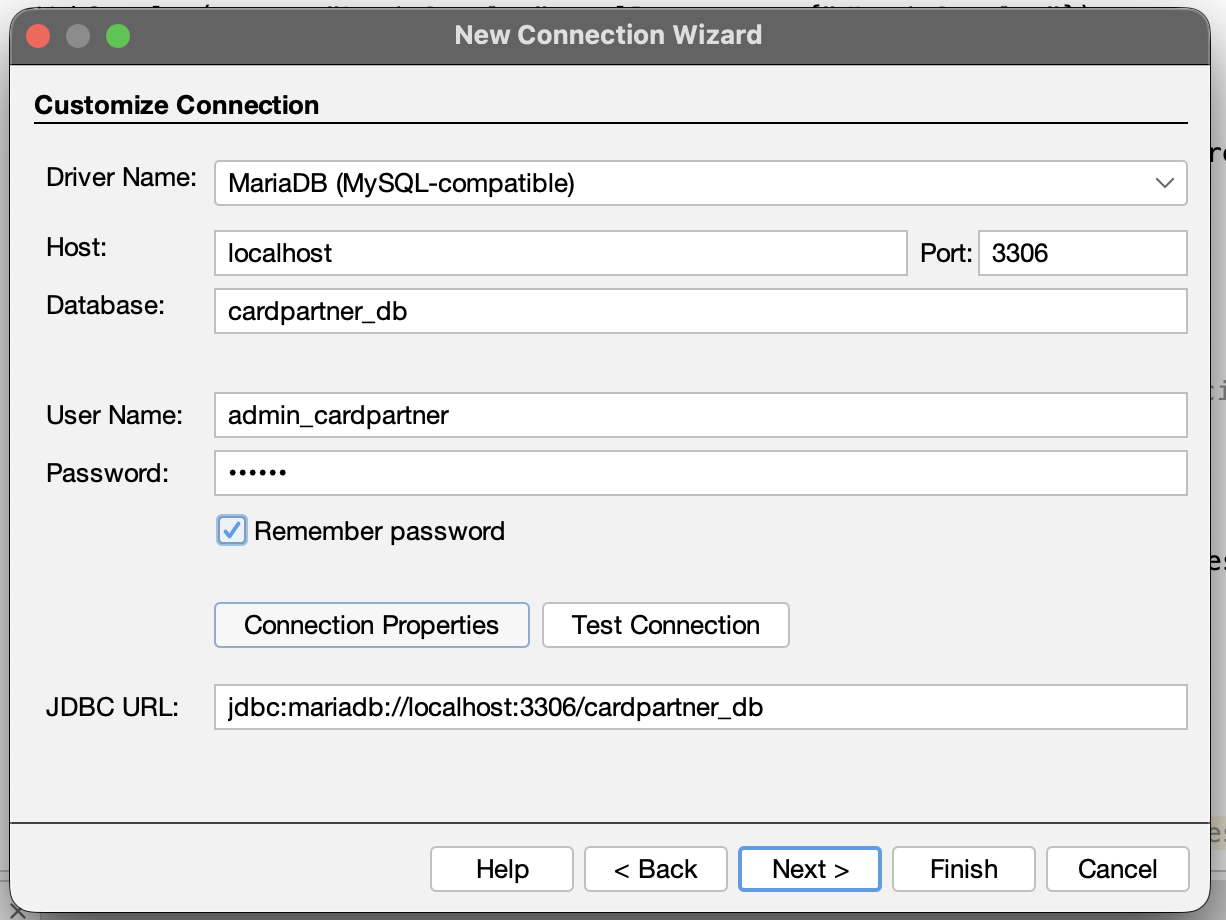
\includegraphics[width=\textwidth]{Recursos/ConexionBBDD.png}
			\caption{Introducimos el nombre de nuestra base de datos (cardpartner\_db) con su usuario (admin\_cardpartner) y la contraseña (123456)}
			
		\end{subfigure}
		
	\end{figure}
	\begin{itemize}
		\item Vamos al menú de Files del editor
		\item Dentro de este menú, buscamos la carpeta que se llame sql 
		\item Ejecutamos los scripts en orden para tener toda la información necesaria en nuestra base de datos.
		\item Ejecutamos la aplicación.
	\end{itemize}
	
	\subsubsection{Usuarios para login}
	Para la funcionalidad de inicio de sesion, se han creado los siguientes usuarios en la base de datos:
	
	\begin{table}[H]
		\centering
		
		\vspace{0.3cm} % Espacio entre caption y tabla
		\begin{tabular}{c c c} 
			\toprule
			\textbf{Apodo} & \textbf{Email} & \textbf{Password} \\
			\midrule
			admin  & admin@test.com        & 123456 \\
			sergio & sergio@test.com       & 123456 \\
			marcos & marcos@test.com       & 123456 \\
			alvaro & admin@cardpartner.com & 123456 \\
			edgar  & edgar@test.com        & 123456 \\
			xabi   & xabi@test.com         & 123456 \\
			\bottomrule
		\end{tabular}
		\caption{Credenciales de usuarios para pruebas de sistema}
		\label{tausuarios_prueba}
	\end{table}
	\newpage
	\section*{Anexo}
	\appendix
	Adjuntamos el código de las modificamos más importantes para que se tenga un acceso más rápido 
	\section{API de las cartas}\label{JAVAAPI}
		\lstinputlisting[language=Java, caption={Clase completa OptcgAPI.}]{CardPartner/src/java/controladores/OptcgAPI.java}
	\section{API de traducción}\label{JAVAGEMINI}
	\lstinputlisting[language=Java, caption={Clase completa OptcgAPI.}]{CardPartner/src/java/controladores/OptcgAPI.java}
	
\end{document}